\chapter{The effect of an S-wave on the angular analysis of \BdToKpill}
\label{chap:swave:theo}

\emph{This chapter is the work of the author except where referenced. This work was published in Ref~\cite{Blake:2012mb}. 
This work was based on Ref.~\cite{LHCb-CONF-2012-008} and uses different values for the angular observables than were measured in the previous chapter. 
This does not affect the conclusions of this chapter since the size of the bias comes from the size of the dilution factor coming from the \kpi S-wave contribution.
%The size of the S-wave contribution used is independant of the measured central values of the angular observables.
}

\section{Introduction}


The \lhcb detector is a single-arm forward spectrometer designed 
for precision measurements of particles containing \bquark quarks~\cite{Alves:2008zz}. 
It is one of the four main experiments at the Large Hadron Collider (\lhc) at the 
European Organisation for Nuclear Research (\cern) in Geneva, Switzerland.
In this chapter the \lhcb detector, its performance and its use to select \BdToKstmm events is shown.
The \lhcb detector is described in Section~\ref{sec:lhcb:det} detailing the sub-detector components
 required for measurements of \bsll decays. % (Section~\ref{sec:lhcb:sub}).
The trigger system used in the \lhcb detector is described in Section~\ref{sec:lhcb:trig} and 
an overview of the software used in \lhcb is given in Section~\ref{sec:lhcb:soft}.
The development of the trigger system used to select \BdToKstmm decays for the 2011 data-taking is presented in Section~\ref{sec:lhcb:trigdev} 
along with the final configuration of the \lhcb trigger system used throughout 2011.
%The high performance of the \lhcb detector throughout 2011 is presented in Section~\ref{sec:lhcb:perf}.

\subsection[CERN]{\cern}

\cern is an international organisation founded in 1954 in order to provide a 
politically neutral place to carry out research in nuclear and particle physics.
At the time of writing, \cern has 20 full member states and there are around ten thousand people associated with science at \cern.
Over the years that \cern has operated, it has contributed to the discovery of neutral currents~\cite{Hasert:1973ff}, 
the electroweak gauge bosons~\cite{Arnison:1983rp,Arnison:1983mk} and recently the Higgs boson~\cite{CMS:2012gu,ATLAS:2012gk}.
\cern is primarily home to the \lhc accelerator complex, which is a proton-proton ($pp$) collider with a circumference
 of 27\km at a depth of 100\m under the the French-Swiss border just outside Geneva.
The \lhc accelerator is built in the tunnel originally used for the \lep accelerator and ran at an energy of 
\sqs=7\tev in 2011.
The injection chain  for the \lhc consists of one linear accelerator and three synchrotrons as shown in Fig.~\ref{fig:lhccomplex}. 
\begin{figure}[tbp]
\centering
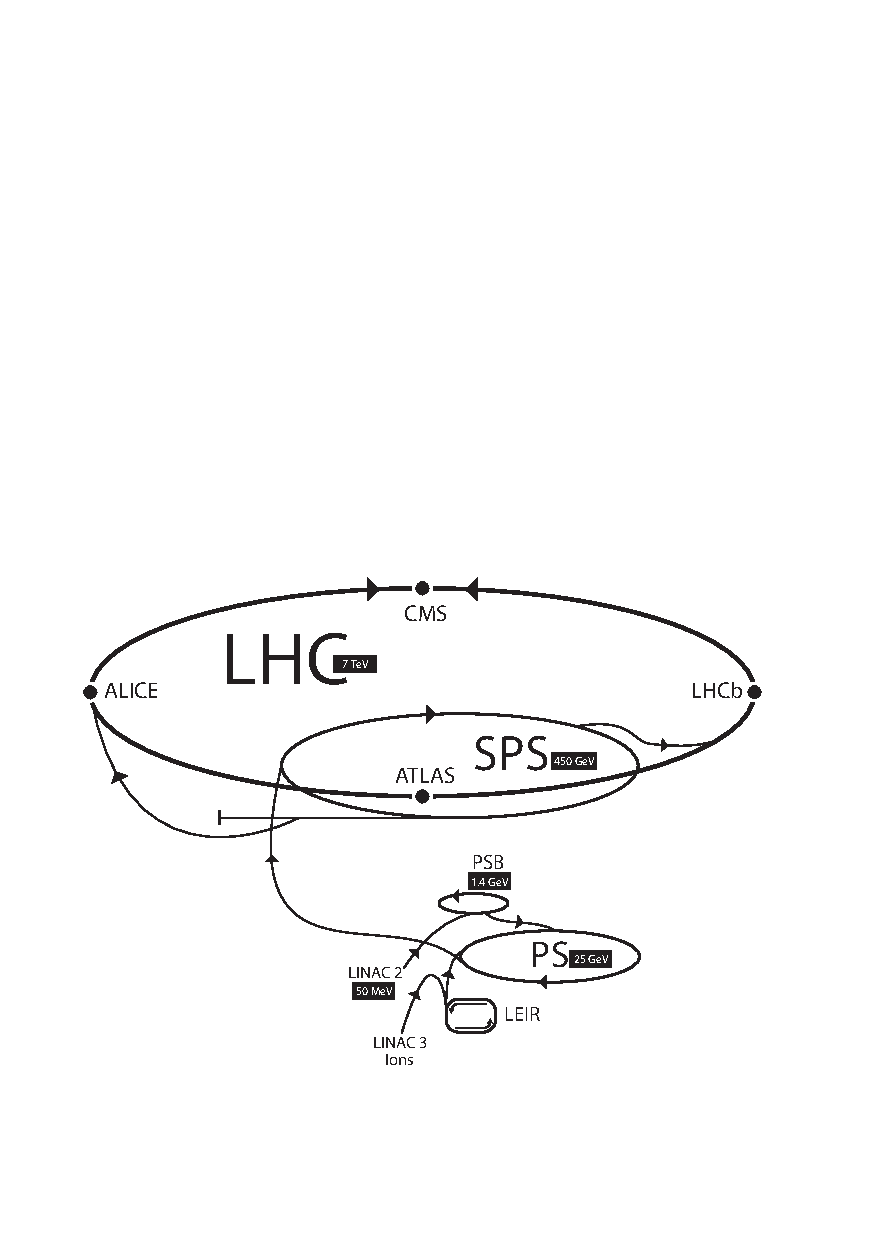
\includegraphics[width=0.48\columnwidth]{chapter3/figs/cern.pdf}
\caption[The \lhc ring.]{A illustration of the the \lhc accelerator complex showing each of the stages in the injection chain 
 for the \lhc ring along with the four main experiments on the \lhc ring~\cite{Lefevre:1092437}. ~\label{fig:lhccomplex} }
\end{figure}
It starts with a linear accelerator which accelerates the protons from rest to 50\mev. 
The synchrotrons increase the beam energy and refine the proton bunches to a configuration suitable for the \lhc. 
Firstly the Proton Synchrotron Booster (PSB) takes the beam from 50\mev to 1.5\gev at which point the 
beam enters the Proton Synchrotron (PS) where the beam energy is increased to 25\gev. 
The beam is then transferred to the Super Proton Synchrotron (SPS) which increases the energy to 450\gev
 before injecting the protons into the \lhc. 
The \lhc accelerates the proton bunches from injection energy at 450\gev to the final collision energy, which was 3.5\tev per beam in 2011 and 4\tev per beam in 2012.
Consolidation upgrades of the \lhc to take place in 2013 and 2014 are expected to increase this collision energy to the design energy of 7\tev per beam.
During operation in 2011-12 there were 1380 proton bunches per beam with a bunch spacing of 50\ns.
There are four main experiments on the \lhc ring, two general purpose detectors (\atlas and \cms), 
along with a heavy-ion experiment (\alice) and a dedicated B-physics experiment (\lhcb).

At the \lhcb interaction point the instantaneous luminosity of the colliding proton bunches 
 is constant at around $\lum\approx3\times10^{32}\cm^2\sec^{-1}$. 
This is significantly below the  \lhc  luminosity, which in 2011 reached over $\lum\approx1\times10^{33}\cm^2\squark^{-1}$.
This luminosity was chosen so that the number of interactions per proton bunch crossing ($\mu$) 
stayed uniform throughout the period of proton collisions for each `fill' of the \lhc.
This ensures that the environment is consistent and has a low multiplicity for reconstruction of \B mesons 
but that there is still a sufficient number of \B meson decays of interest for a given number of collisions.

The production of \bbbar pairs in $pp$ interactions is governed predominantly 
by gluon fusion, $gg\to\bbbar$.
The collision of partons of unequal energy and a momentum boost along the direction of the collision results in \bbbar pairs 
that are produced at small angles to the beam axis.
The angular distribution of \bbbar production is shown in Fig.~\ref{fig:lhcb:bbbar}.
\begin{figure}[tbp]
\centering
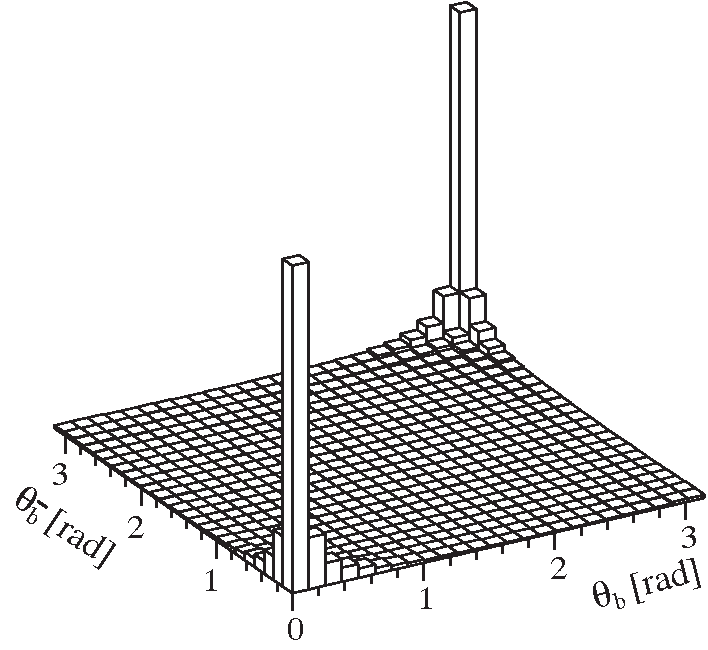
\includegraphics[width=0.48\columnwidth]{chapter3/figs/angular.pdf}
\caption[ $b\bar{b}$ production at the LHC ]{The angular distribution of \bbbar pairs in terms of the polar angle from the beam axis.
The \bbbar pairs are largely produced within a very small opening angle hence the development of \lhcb as a forward spectrometer
~\cite{Alves:2008zz}.~\label{fig:lhcb:bbbar} }
\end{figure}
The \bbbar cross section at \sqs=7\tev is 75\mub within the \lhcb acceptance~\cite{LHCb-PAPER-2010-002}. 
%This corresponds to around $10^7$ \bbbar pairs produced in the 2011 year of data-taking.
In total the experiment recorded an integrated luminosity of 1.0\invfb in 2011 that could be used for further analysis.
The increase in integrated luminosity throughout the year can be seen in Fig.~\ref{fig:lhcb:intlumi} along with the technical stops
 and periods of machine development.
\begin{figure}
\centering
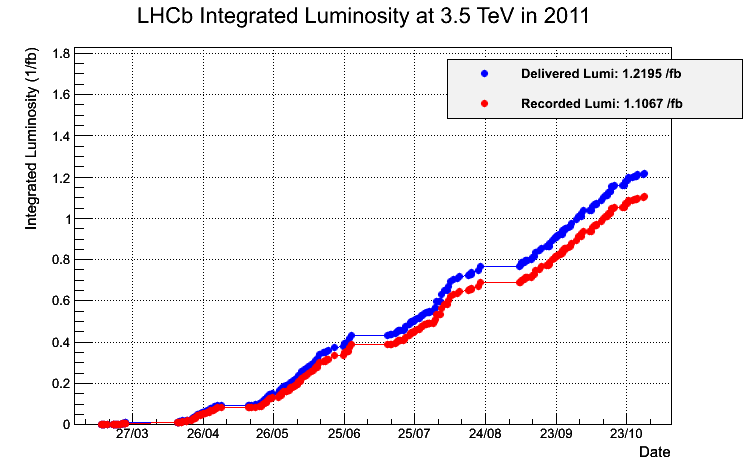
\includegraphics[width=0.66\columnwidth]{chapter3/figs/2011IntegratedLumiLHCbTime_NoPie.png}
\caption{The integrated luminosity recorded by \lhcb during 2011~\cite{OpsPlots}.~\label{fig:lhcb:intlumi} }
\end{figure}


\section{Theoretical formalism of the \psq spectrum}
\label{sec:swave:theo}

The \BdToKpill angular distribution can be expressed for multiple S-wave states 
as described in Section~\ref{sec:fullangdist} and Ref.~\cite{Lu:2011jm}.
For \kpi masses below  
$1200\mev$,  the %it can be seen from the previous section that
contribution to the amplitudes from the higher $\Kstarz$ states is 
small enough that it can be ignored.
In order to understand the S-wave contribution to the \BdToKpill angular distribution
 close to the $\Kstarz(892)$ so only the $J=0,1$ terms in
the sums of Eq.~\ref{eq:amp} were considered.

The S-wave contribution to these amplitudes only enters in the amplitude $\mathcal{A}_{0}$, 
\begin{align}
\label{eq:amps1}
\mathcal{A}_{H0} &= \sqrt{\frac{1}{4\pi}} A_{0H0} + \sqrt{\frac{3}{4\pi}} A_{1H0} \ctk    \\
\mathcal{A}_{H||} &= \sqrt{\frac{3}{8\pi}} A_{1H||} \stk  \\
\mathcal{A}_{H\bot} &= \sqrt{\frac{3}{8\pi}} A_{1H\bot} \stk   
\end{align}
where the spherical harmonics are expanded, leaving the phase space factor, 
the propagator and the matrix element as part of the spin-dependent amplitudes
\begin{equation}
\label{eq:amps2}
\begin{split}
A_{0,H,0} &\propto \rho(\psq,\qsq) \times M_{0,H,0} (\qsq) \times  P_0(\psq) , \\
A_{1,H,0} &\propto  \rho(\psq,\qsq) \times  M_{1,H,0} (\qsq) \times  P_1(\psq) , \\
A_{1,H,\bot} &\propto  \rho(\psq,\qsq)  \times M_{1,H,\bot} (\qsq) \times  P_1(\psq) , \\
A_{1,H,||} &\propto  \rho(\psq,\qsq) \times M_{1,H,||} (\qsq) \times P_1(\psq) ,  
\end{split}
\end{equation}
where the first index denotes the spin. 
The normalisation from the three-body phase space factor is described in more detail below.

\subsection{Phase space factors}
\label{sec:swave:phasespace}

The phase space for the four-body decay \BdToKpill can be described by three three-body phase space factors
\begin{align}
\rho(\Bd\to(\kpi)(\ellell)) \times \rho((\kpi)\to\kaon\pion) \times \rho((\ellell)\to\ellp\ellm) \, .
\end{align}
The three-body phase space factor is
\begin{align}
\rho(a \to b c ) = \left(\frac{\sqrt{ \lambda ( a, b , c ) }}{8\pi a^2}\right)^{2J+1}
\end{align}
where $\lambda(a,b,c) = \left(a^2+b^2+c^2\right)^2-4b^2c^2$ is the triangle function and $J$ is
 the difference in spin of $a$ and $b$. 
%The \qsq-dependent phase space factor is assumed to be fixed and the combination of \qsq and \psq dependence is not considered in this chapter.
The phase space for \BdToKpill as a function of \psq and \qsq is given in Fig.~\ref{fig:phasespace}. 
\begin{figure}[tb]
\centering
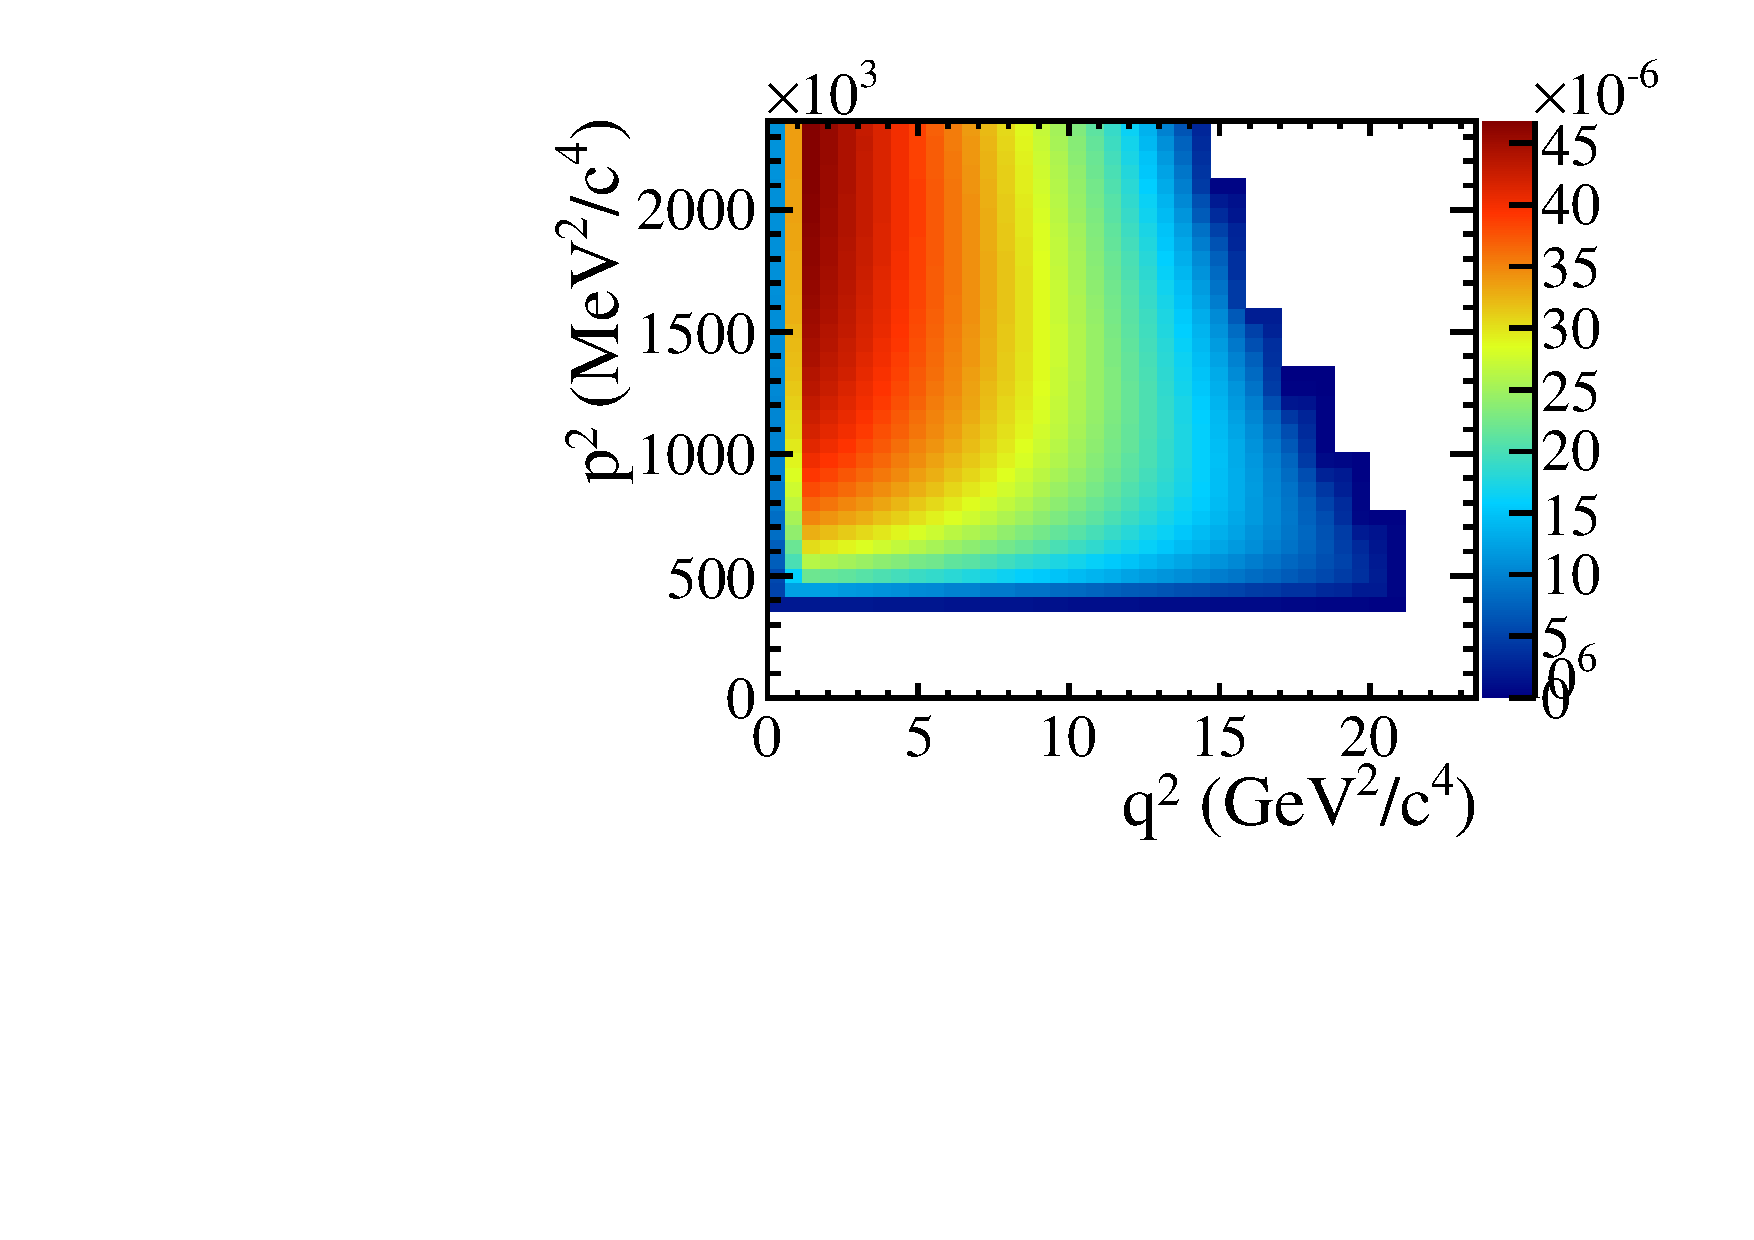
\includegraphics[width=0.48\columnwidth]{chapter6/figs/test_phasespace_psq_qsq.pdf}
\caption[ The phase space for \BdToKpill as a function of \psq and \qsq.   ]
{ The phase space for \BdToKpill as a function of \psq and \qsq. 
The kinematic edge for the high mass \Kstarz states is clearly seen. ~\label{fig:phasespace} }
\end{figure}
The region of S-wave and P-wave interference is mainly at \psq values below $1200^2\mevmevcccc$
 where there is a small reduction in phase space at high \qsq.

\subsection{Propagator functions}
\label{sec:swave:propfunctions}

The propagator for the P-wave is described by a relativistic Breit-Wigner distribution with the amplitude given by
\begin{align}
\label{eq:rbw}
P_1(\psq) = \frac{ m_{\Kstarzo} \Gamma_{\Kstarzo}(\psq)}{ m_{\Kstarzo}^2 - \psq + i \  m_{\Kstarzo} \Gamma_{\Kstarzo}(\psq)} 
\end{align}
where  $m_{\Kstarzo}$ is the resonant mass and 
\begin{align}
\Gamma_{\Kstarzo}(\psq) = \Gamma_{\Kstarzo}^0 \left( \frac{ t }{t_0} \right)^{2J+1} \left( \frac{ m_{\Kstarzo} }{ p } \right) \frac{ B\left(tR_P\right) }{ B\left(t_0R_P\right) }
\end{align}
the running width. Here $t$ is the \Kp momentum in the rest frame of the \kpi system and $t_0$ is t evaluated at the \kpi pole mass.
$B$ is the Blatt-Weisskopf damping factor~\cite{Blatt:628052} with a radius $R_P$.
For P-wave the value of $R_P$ is taken to be $3.0\gev^{-1}$  (from Ref~\cite{Aubert:2008aa}). 
The amplitude can be defined in terms of a phase ($\delta$) through the substitution
\begin{align}
\cot \delta = \frac{  \psq - m_{\Kstarzo}^2 }{  \Gamma_{m_{\Kstarzo}}(\psq) m_{\Kstarzo} }
\end{align}
to give the polar form of the relativistic Breit-Wigner propagator 
\begin{align}
P_1(\psq) =   \frac{1}{\cot\delta - i } 
\end{align}
The LASS parametrisation of the S-wave~\cite{Aston:179353} 
can be used to describe a generic \kpi S-wave.  
In this parametrisation, the S-wave propagator is defined as 
\begin{align}
\label{eq:lass}
P_0(\psq) = \frac{p}{t} \left( \frac{1 }{ \cot\delta_B - i } + e^{2i\delta_B}( \frac{1}{\cot\delta_R - i }) \right)
\end{align}
where the first term is an empirical term from inelastic scattering and the second term is
 the resonant contribution with a phase factor to retain unitarity.
The first phase factor is defined as
\begin{align}
\cot\delta_B = \frac{1}{ta} + \frac{1}{2}rt ,
\end{align}
where $r$ and $a$ are free parameters and $t$ is defined previously,
while the second phase factor describes the $\Kstarzz(1430)$
 through 
\begin{align}
\cot\delta_R = \frac{ \psq - m_{\mathrm{S}}^2 }{ \Gamma_{\mathrm{S}}(\psq) m_{\mathrm{S}}  }.
\end{align}
Here, $m_{\mathrm{S}}$ is the S-wave pole mass and $\Gamma_{\mathrm{S}}$ is the 
running width using the pole mass of the $\Kstarzz(1430)$.
The overall strong phase shift between the results from the LASS scattering experiment and 
measured values for \Bd\to\jpsi\kpi has been found to be consistent with $\pi$~\cite{Aubert:2004cp}. 
The parameters for the \psq spectrum used are given in Table~\ref{tbl:params}.
\begin{table}[tb]
\centering
\caption[ Parameters of the \kpi resonances used to generate toy data sets.    ]
{Parameters of the \kpi resonances used to generate toy data sets. The \Kstar masses and widths 
are taken from Ref.~\cite{PDG2012} and the \Kstarzo Blatt-Weisskopf radius and 
the LASS parameters are taken from Ref.~\cite{Aubert:2008aa}~\label{tbl:params}}
\begin{tabular}{|c|c|c|c|c|c|c|}
\hline
State. & mass & $\Gamma$ & R & $r$ & $a$ & $ \delta_{\mathrm{J}} $ \\
  & (\mev) & $(\mev)$ & ($\gev)^{-1}$ & $(\gev)^{-1}$ & $(\gev)^{-1}$ &  \\
\hline
\Kstarzz & $ 1425  \pm 50 $ & $ 270 \pm 80 $ & $1.0$ & $1.94$ & $1.73$ &  $\pi$ \\
\Kstarzo & $ 894.94  \pm 0.22$ & $ 48.7 \pm 0.8 $ & $3.0$  & \  & \ & 0  \\
\Kstarzt & $ 1432.4  \pm 1.3$ & $ 109 \pm 5 $ & $1.5$  & \  & \ & 0  \\
\hline
\end{tabular}
\end{table} 

\subsection{Angular coefficients}
The angular terms modified by the inclusion of the S-wave are $I_{1,2,4,5,7,8}$ and  
the complete set of angular terms expressed in terms of the spin-dependent amplitudes
are
%Some important features from the angular coefficiencts can by understoof by examination of $I_1^c$, given as
\begin{align}
\label{eq:angularcoeff1}
I_1^c &=  \frac{1}{4\pi} |A_{0L0}|^2 + \frac{3}{4\pi} |A_{1L0}|^2\ctksq + 2 \frac{\sqrt{3}}{4\pi} |A_{0L0}||A_{1L0}|\cos\delta_{0,0}^L \ctk + (L\to R) \frac{}{}  \nonumber \\
I_1^s &= \frac{3}{4} \frac{3}{8\pi} \left( |A_{1L||}|^2 + |A_{1L\bot}|^2 + (L\to R) \right) \frac{}{}\stksq \nonumber   \\
I_2^c &= - I_1^c , \qquad \, I_2^s = \frac{1}{3} I_1^s \nonumber\\ 
I_3 &= \frac{1}{2}  \frac{3}{8\pi}  \left( |A_{1L\bot}|^2 - |A_{1L||}|^2 + (L\to R) \right) \stksq  \frac{}{}\nonumber\\
I_4 &= \frac{1}{\sqrt{2}} \left[  \frac{1}{4\pi}\sqrt{\frac{3}{2}}\Re( A_{0L0}A_{1L||}^{*}) \cos\delta_{0,||}^L \stk  \right. \frac{}{} \nonumber\\
      &+ \left. \frac{3}{4\pi}\sqrt{\frac{1}{2}}\Re( A_{1L0}A_{1L||}^{*})  \stk \ctk  + ( L \to R )  \right] \frac{}{}\nonumber \\
I_5 &= \frac{1}{\sqrt{2}} \left[  \frac{1}{4\pi}\sqrt{\frac{3}{2}}\Re( A_{0L0}A_{1L\bot}^{*}) \cos\delta_{0,\bot}^L \stk  \right. \frac{}{} \nonumber\\
    &+  \left.  \frac{3}{4\pi}\sqrt{\frac{1}{2}}\Re( A_{1L0}A_{1L\bot}^{*})  \stk \ctk  - ( L \to R )  \right] \frac{}{} \\
I_6 &= 2  \frac{3}{8\pi} \left( \Re(A_{1L||}A_{1L\bot}^{*}) - (L\to R) \right) \stksq \frac{}{} \nonumber  \\
I_7 &= \frac{1}{\sqrt{2}} \left[  \frac{1}{4\pi}\sqrt{\frac{3}{2}}\Im( A_{0L0}A_{1L||}^{*}) \cos\delta_{0,||}^L \stk \right. \frac{}{}  \nonumber\\ 
    & + \left.   \frac{3}{4\pi}\sqrt{\frac{1}{2}}\Im( A_{1L0}A_{1L||}^{*})  \stk \ctk   - ( L \to R )  \right] \frac{}{} \nonumber \displaybreak[1]  \\
I_8 &= \frac{1}{\sqrt{2}} \left[  \frac{1}{4\pi}\sqrt{\frac{3}{2}}\Im( A_{0L0}A_{1L\bot}^{*}) \cos\delta_{0,\bot}^L \stk \right. \frac{}{} \nonumber\\
 &  + \left.    \frac{3}{4\pi}\sqrt{\frac{1}{2}}\Im( A_{1L0}A_{1L\bot}^{*})   \stk \ctk  + ( L \to R )  \right]  \frac{}{} \nonumber \\
I_9 &=    \frac{3}{8\pi} \left(  \Im(A_{1L||}A_{1L\bot}^{*}) + (L\to R) \right) \stksq \frac{}{}\nonumber
\end{align}
The interference term of $I_1$ shows how this parametrisation includes the
 strong phase difference between the S- and P-wave state. 
The left handed part of the interference term for $I_1$ can be written as 
\begin{align}
2 |A_{0L0}||A_{1L0}|\cos\delta_{0,0}^L \propto 2\, |M_{0,L,0}||P_0(\psq)||M_{1,L,0}||P_1(\psq)| \cos( \delta_{0,0}^L ) 
\end{align}
where 
\begin{align}
 \delta_{0,0}^L =  \delta_{M_{0L0}} + \delta_{P_0} - \delta_{M_{1L0}} - \delta_{P_1}  .
\end{align}
where $\delta_{M_{JL0}}$ is the phase of the  longitudinal matrix element and 
$\delta_{P_J}$ is the phase of the propagator.
The phases in the interference terms for $I_{4,5,7,8}$ can be similarly defined.
For real matrix elements,~i.e.~nearly true in the Standard Model, the phases are 
equal for both handed interference terms $\delta^L = \delta^R$.
The phase difference between the S-wave and the P-wave propagators can be 
expressed as a single strong phase, $\delta_{\mathrm{S}}$.



\subsection{The \psq spectrum for \BdToKpill}

The \psq spectrum for the  \BdToKpill angular distribution can
 be calculated by summing over the S- and P-waves and integrating 
out the \ctl, \ctk and $\phi$ dependence. This is illustrated in 
Fig.~\ref{fig:psqat6}
\begin{figure}[tb]
\centering
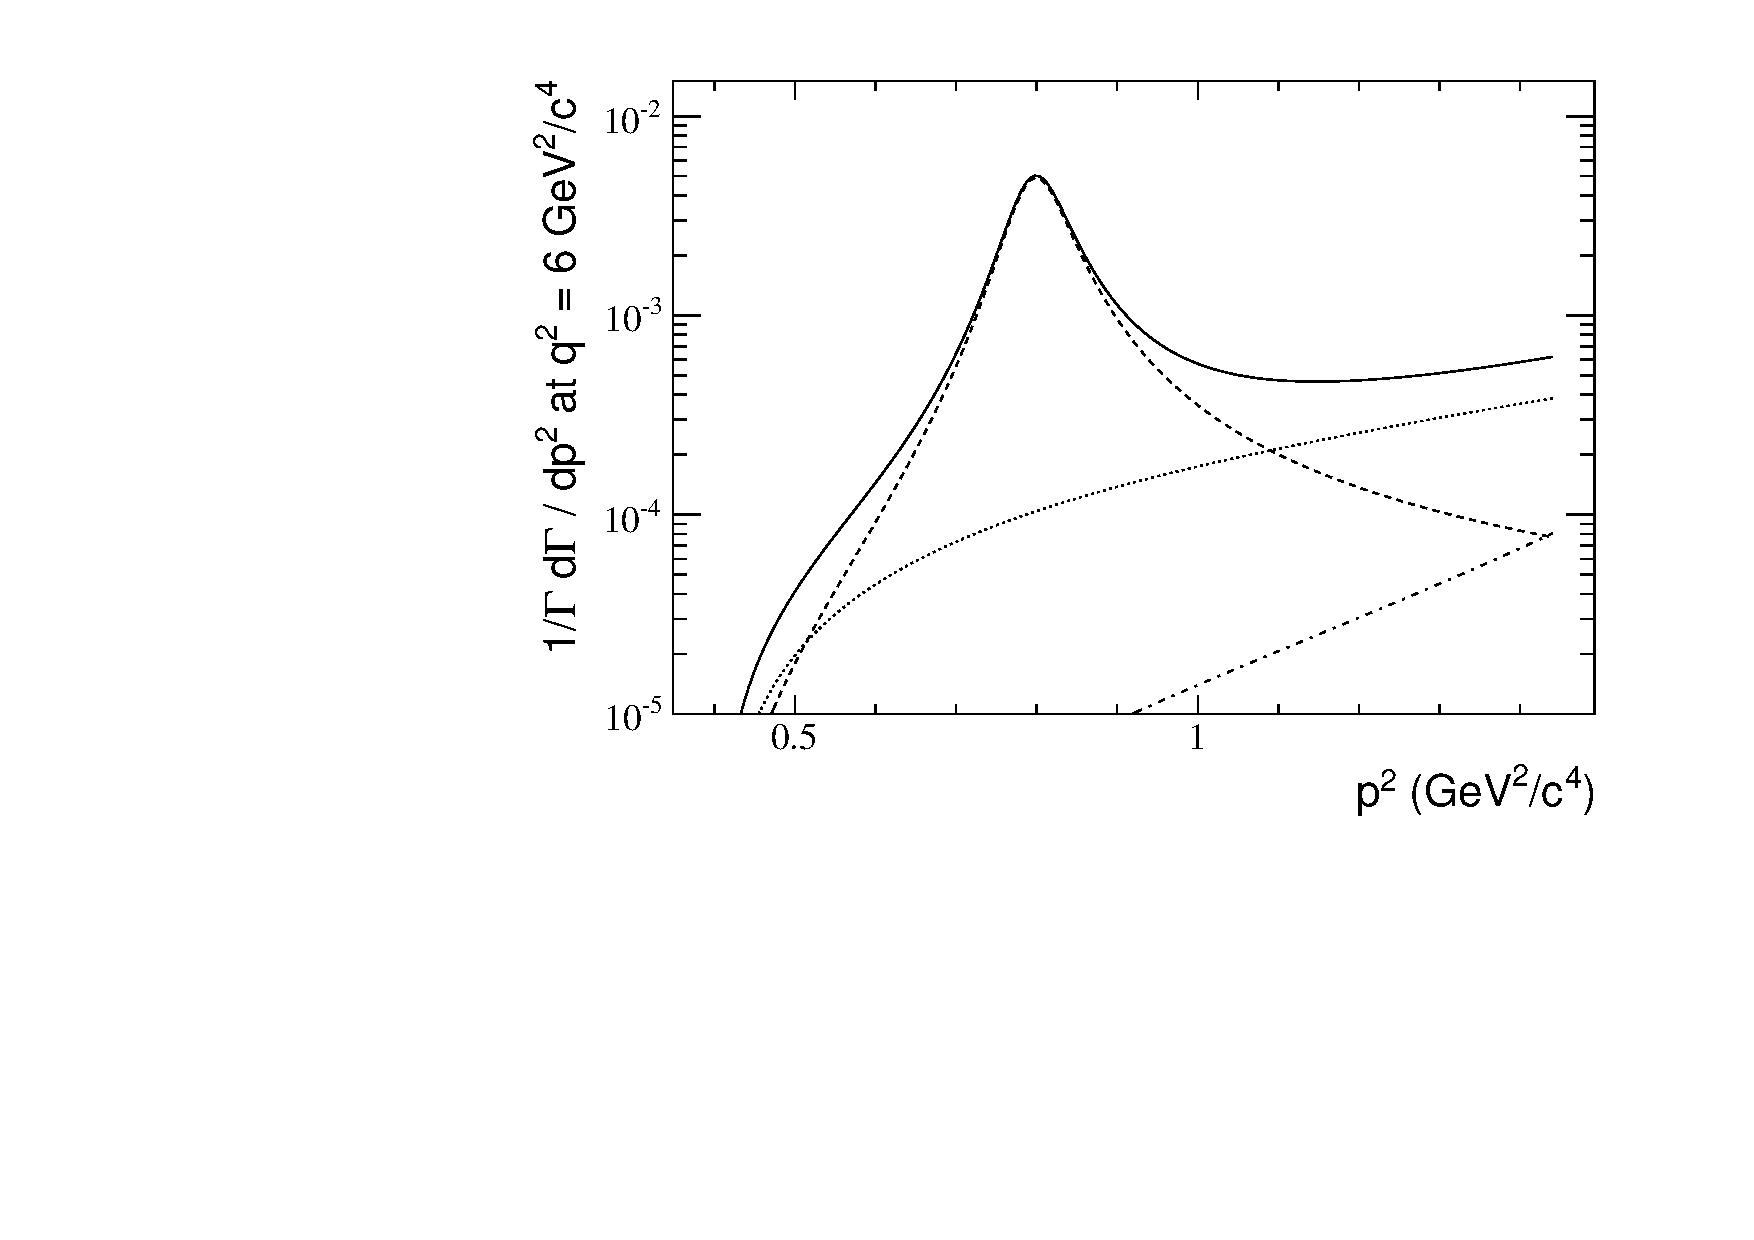
\includegraphics[width=0.66\textwidth]{chapter6/figs/calc_psq_branch_frac_logy.pdf}
\caption[  An illustration of the \psq spectrum for the P-wave (dashed) and the S-wave (dotted).    ]
{ An illustration of the \psq spectrum for the P-wave (dashed) and the S-wave (dotted). 
The total distribution from both states  is the 
solid line. The values were calculated at $q^2 = 6 \gev^2$ by
 integrating out the angular distribution of \BdToKpill using equal 
matrix elements for each state. The S-wave fraction here is 16\% between $800<p<1000 \mev$~\label{fig:psqat6} } 
\end{figure}
where the matrix elements from 
Refs.~\cite{Egede:2008uy,Egede:2010zc} at a \qsq value of $6\gev^2$ are used. 
Here the S-wave amplitude is assumed to be equivalent to the longitudinal P-wave amplitude.
The S-wave fraction in the $800 < p < 1000\mev$ window around the P-wave 
is calculated to be 16\% when using this approximation.
The size of the S-wave fraction, the P-wave fraction and the interference fraction w.r.t the total branching fraction
are given in Fig.~\ref{fig:fracat6}.
\begin{figure}[tb]
\centering
\subfigure[]{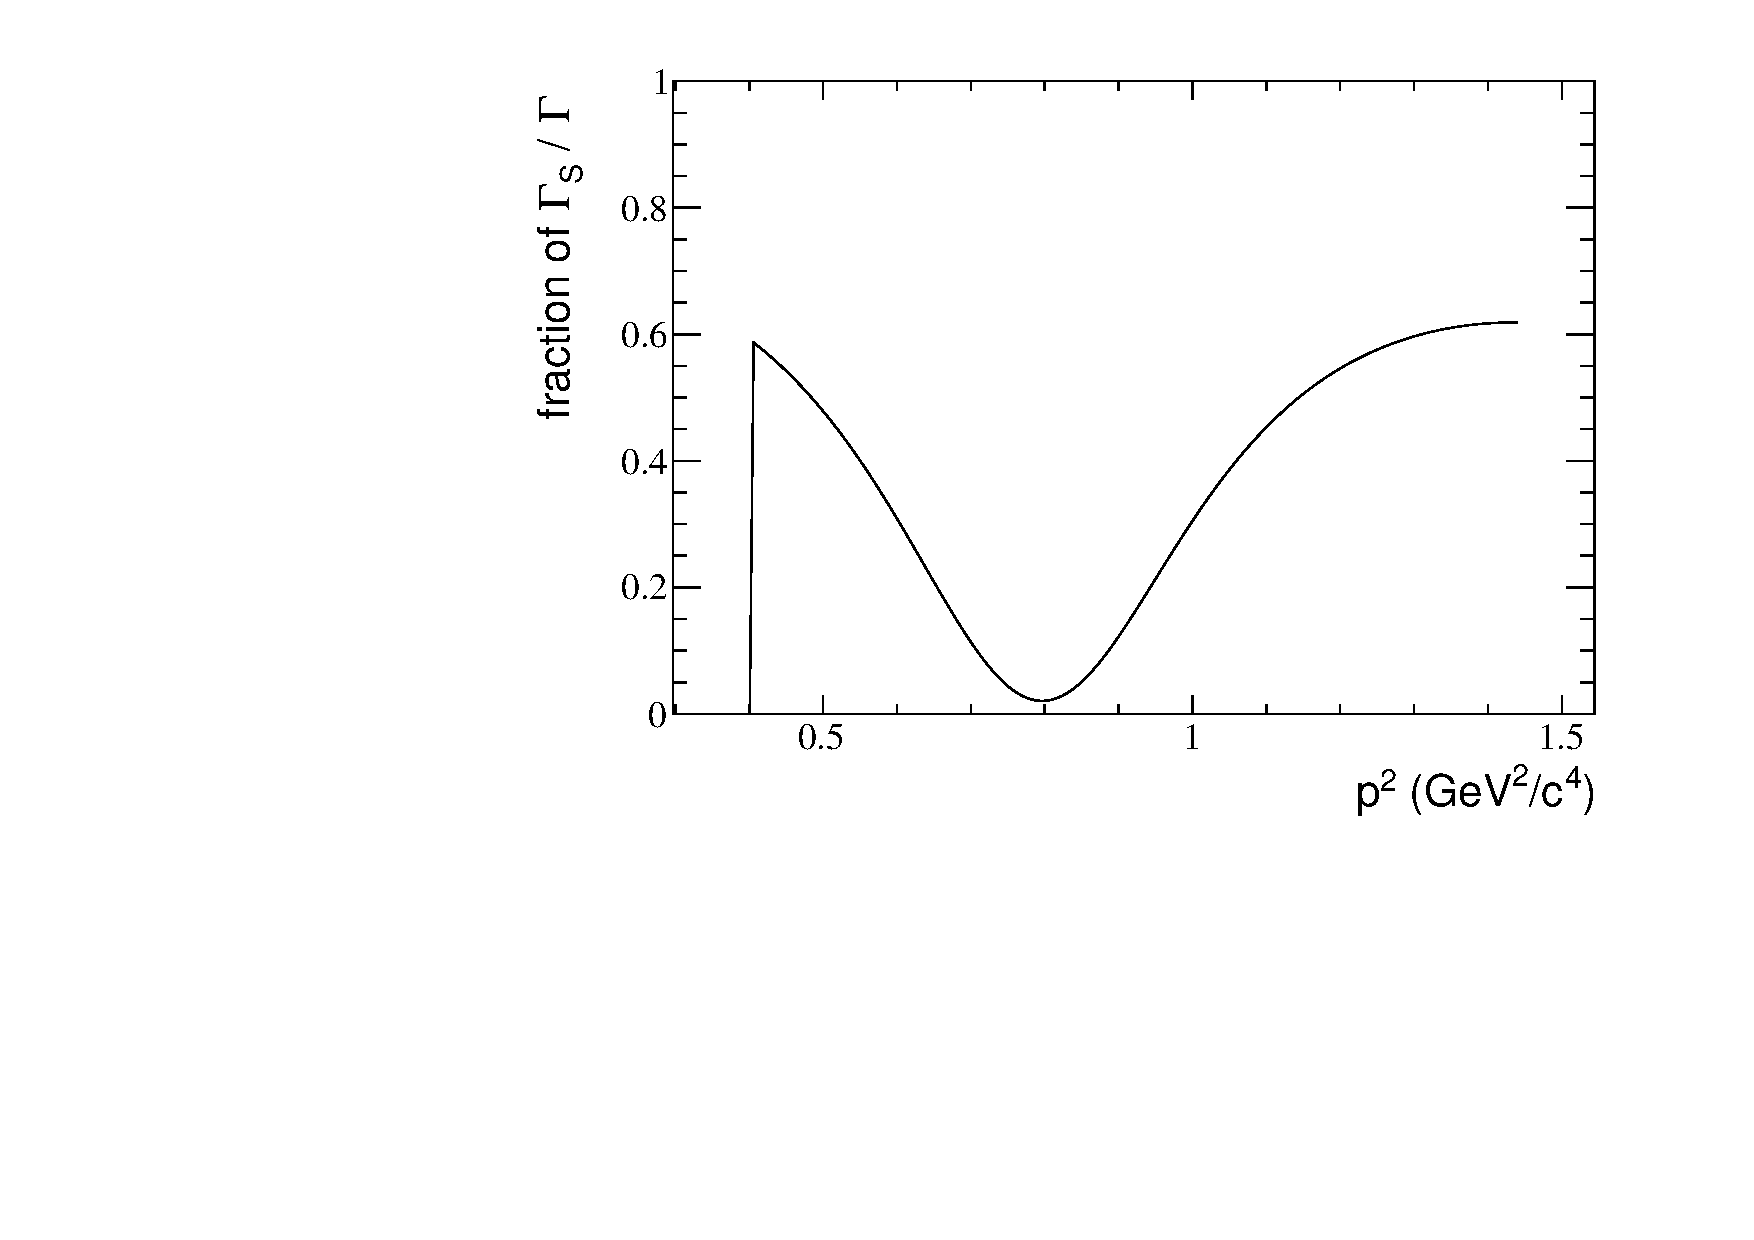
\includegraphics[width=0.48\textwidth]{chapter6/figs/calc_psq_branch_frac_S.pdf}}
\subfigure[]{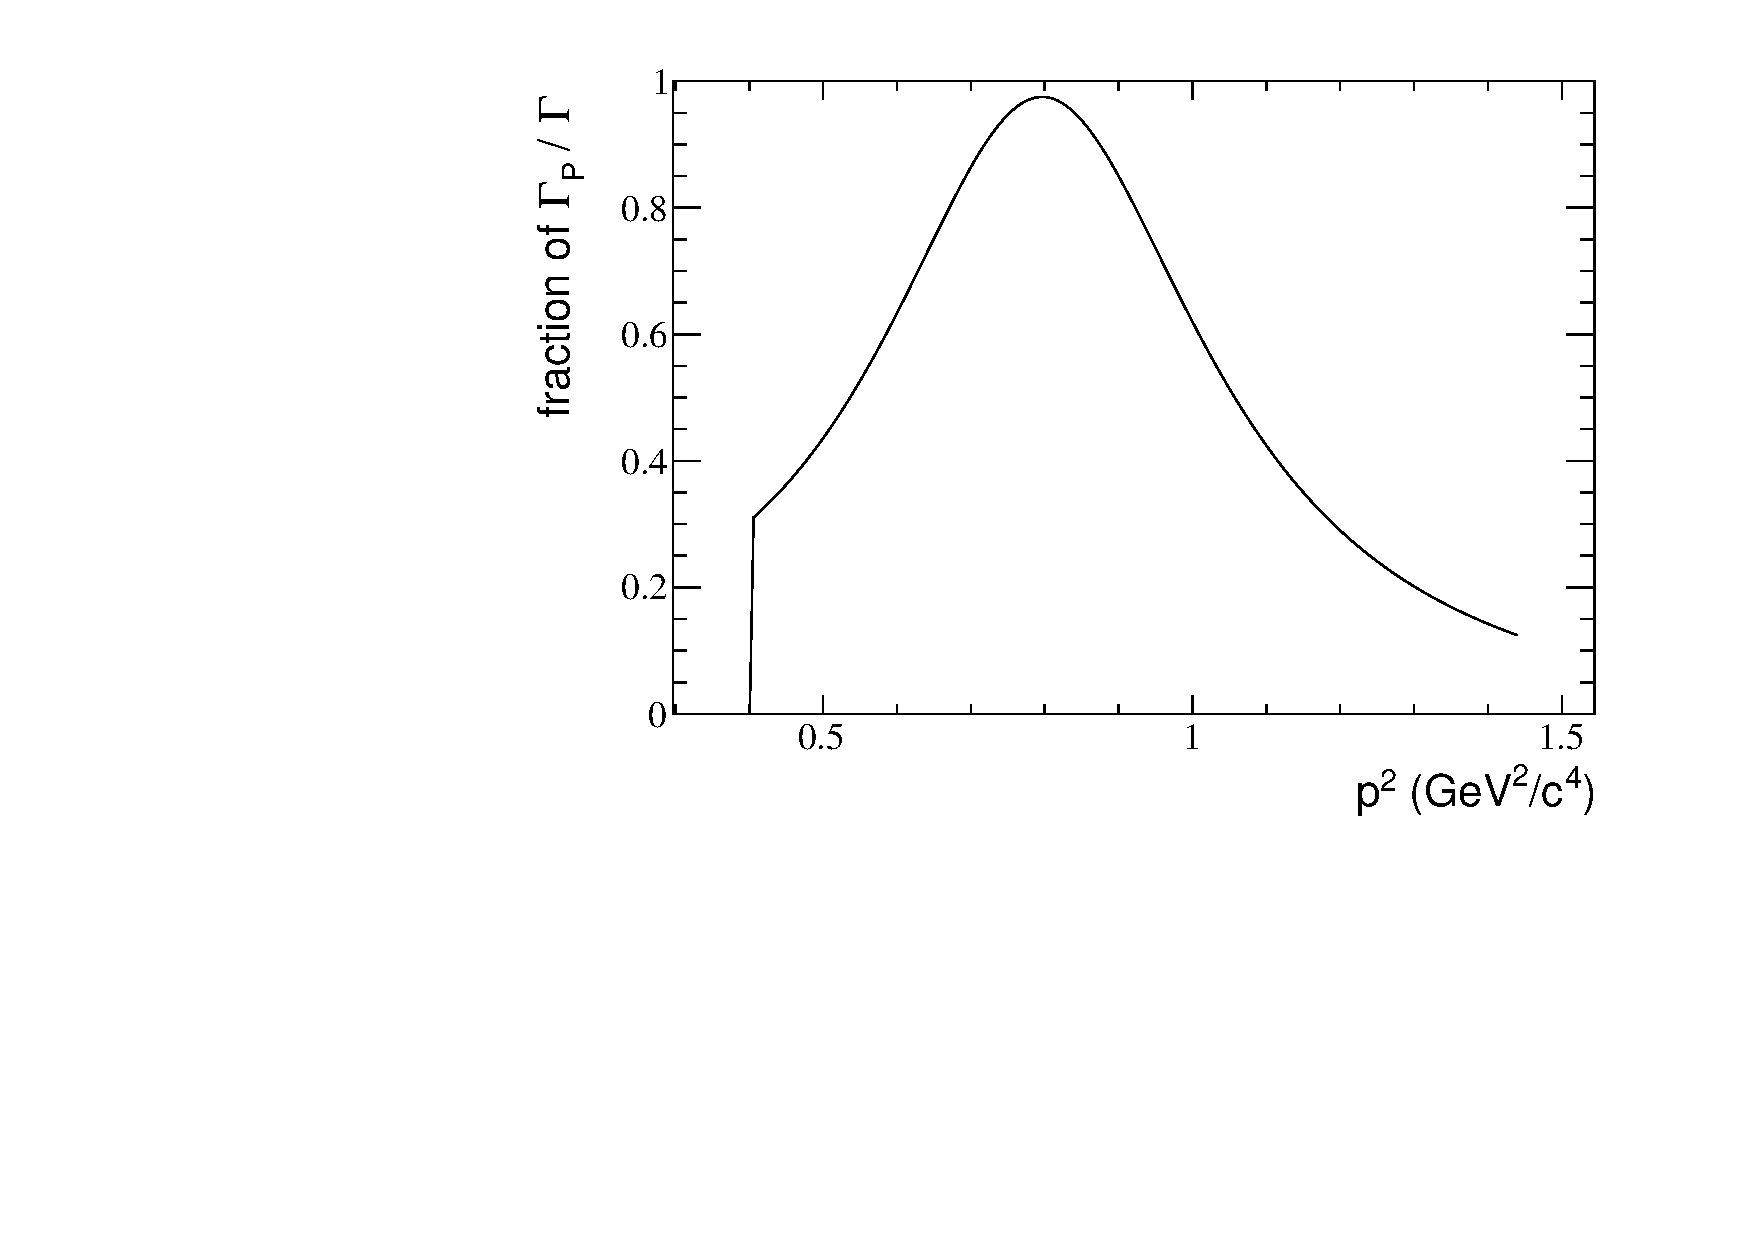
\includegraphics[width=0.48\textwidth]{chapter6/figs/calc_psq_branch_frac_P.pdf}}
\subfigure[]{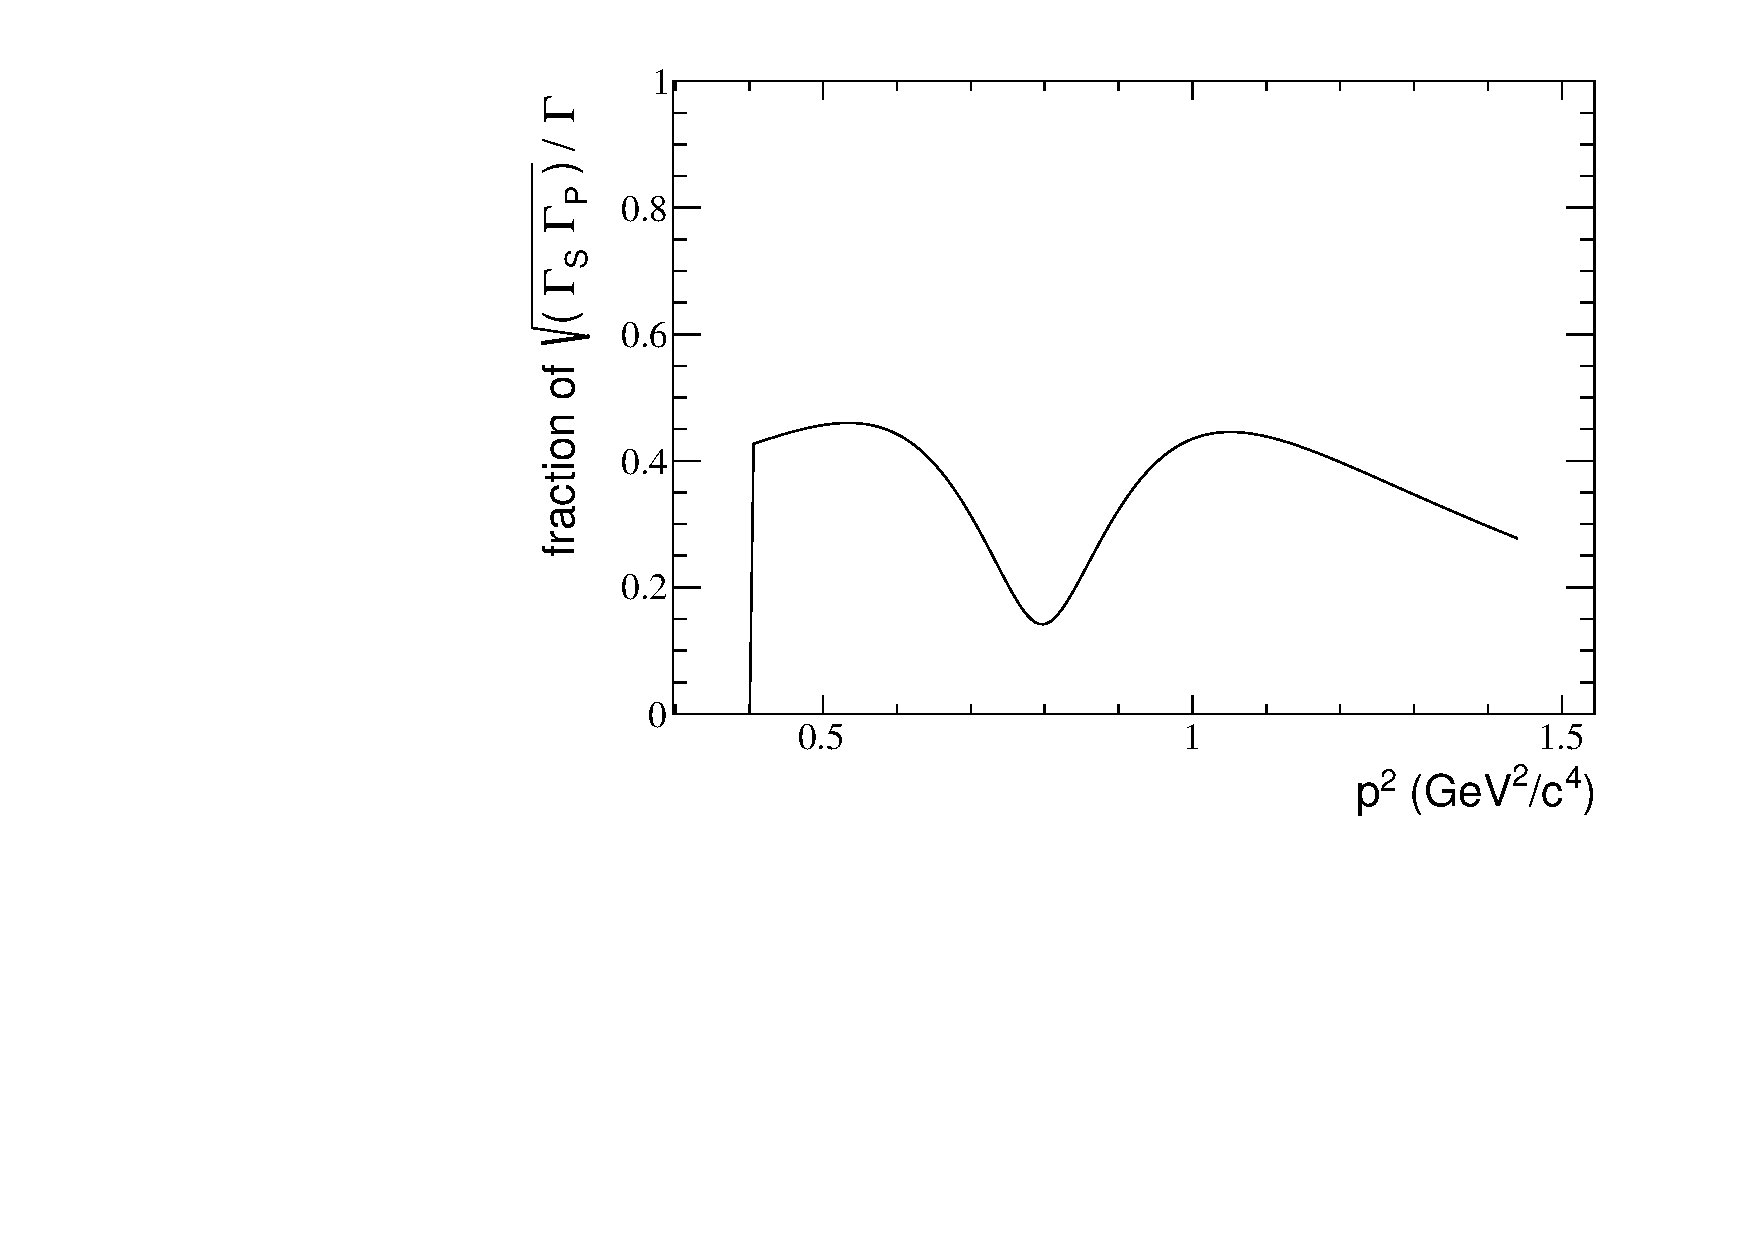
\includegraphics[width=0.48\textwidth]{chapter6/figs/calc_psq_branch_frac_int.pdf}}
\caption[  An illustration of the size of the S-wave, P-wave and S$\leftrightarrow$P-wave
 interference fractions with respect to the total branching fraction. ]
{ An illustration of the size of the S-wave, P-wave and S$\leftrightarrow$P-wave
 interference fractions with respect to the total branching fraction. 
The values were calculated at $q^2 = 6 \gev^2$ by
 integrating out the angular distribution of \BdToKpill using equal 
matrix elements for each state.~\label{fig:fracat6} } 
\end{figure}
As will be seen later there are no interference terms left in the angular distribution after the integral
 over \ctk.




\section{Angular observables}
\label{sec:kstmm:obs}

The contributions from the Wilson coefficients defined above
 can be measured by measuring the transversity amplitudes
 through an angular analysis of the \BdToKstll angular distribution.
Direct measurements of the transversity amplitudes are dependent on the values of the form factors
 which have a significant theoretical uncertainty.
To mitigate these uncertainties and allow measurements of the Wilson coefficients, angular observables
can be constructed from the transversity amplitudes that are independent of the two heavy-to-light form factors.
Many angular observables have been proposed for the decay 
\BdToKstll~\cite{Kruger:2005ep,AltmannshoferBall,Egede:2008uy,Bobeth:2010wg,Matias:2012xw}. 
These observables are combinations of the amplitudes which both minimise the uncertainty from the form factors 
and maximise the contribution from new physics models. 
So far the forward-backward asymmetry (\AFB), the fraction of the \Kstarz longitudinal polarisation (\FL ) 
and two combinations of the transverse amplitudes (\AT2 and \AIm ) have been 
measured~\cite{Aaltonen:2011cn,Aubert:2007hz,Aaltonen:2011ja,Aubert:2008ju,PhysRevLett.103.171801}.

\subsection{P-wave observables}

These observables are constructed from combinations of amplitudes and
are normalised to the sum of amplitudes for the P-wave state, given as 
\begin{align}
|A_{10}|^2 + |A_{1||}|^2 + |A_{1\bot}|^2 \, ,
\end{align}
where the generic combination of amplitudes $A_{Ji}A_{Ji}^{*}$ is defined for a spin $J$ and a polarisation (0,$||$,$\bot$) as
\begin{align}
\label{eq:ampsq}
A_{Ji} A_{Ji}^{*} &= A_{JiL} A_{JiL}^{*} + A_{JiR} A_{JiR}^{*} \, .
\end{align}
The forward-backward asymmetry of the dilepton system, \AFB, enters in the angular coefficient $I_6$ and
is defined in terms of the amplitudes as
\begin{align}
\label{eq:theoafb}
\AFB(\qsq) &= \frac{3}{2} \frac{  \Re(A_{1L||}A_{1L\bot}^{*}) - 
\Re(A_{1R||}A_{1R\bot}^{*})}{|A_{10}|^2 + |A_{1||}|^2 + |A_{1\bot}|^2 } \, .
\end{align}
In a similar way, \FL, \OS3 and \OS9 are defined as
\begin{equation}
\begin{split}
\FL(\qsq) &= \frac{  |A_{10}|^2 } {|A_{10}|^2 + |A_{1||}|^2 + |A_{1\bot}|^2} \\
\OS3 (\qsq) &= \frac{ |A_{1\bot}|^2 - |A_{1||}|^2 }{ |A_{10}|^2 + |A_{1||}|^2 + |A_{1\bot}|^2} \\
\OS9 (\qsq) &= \frac{  \Im(A_{1L||}A_{1L\bot}^{*}) - \Im(A_{1R||}A_{1R\bot}^{*}) }{|A_{10}|^2 + |A_{1||}|^2 + |A_{1\bot}|^2} 
\end{split}
\end{equation}
where \OS3 and \OS9 are related to the angular coefficients $I_3$ and $I_9$ respectively.
These theoretical observables are normalised to the sum of the P-wave amplitudes
and the factorisation of the amplitudes into matrix elements and the 
propagators removes the \psq dependence from these theoretical observables. 

In terms of the angular distribution, \AFB can also be expressed 
as the difference 
between the number of `forward-going' \mup and the number of 
`backward-going' \mup in the rest frame of the \Bd,
\begin{align}
\label{eq:expafb}
\left[ \int_0^1 - \int_{-1}^0 \right]  \text{d}\ctl
\frac{\text{d}\Gamma}{\text{d}\qsq \text{d}\ctl} / 
\frac{\text{d}\Gamma}{\text{d}\qsq} \, ,
\end{align}
which explains the name of the observable. 

\subsection{Transverse observables}
\label{sec:kstmm:reparam}

Angular observables which are normalised to only the transverse helicity amplitudes have
 been studied with the additional aim of reducing the theoretical uncertainties~\cite{Melikhov:1998cd,Kruger:2005ep}.
This is achieved by separating out the dependence on the  longitudinal amplitudes and their form factors from the calculation.
The main transverse observable is \AT2 which comes from the angular coefficient $I_3$,
\begin{align}
\AT2 (\qsq) &=  \frac{ |A_{1\bot}|^2 - |A_{1||}|^2  }{ |A_{1\bot}|^2 + |A_{1||}|^2 }  \, .
\end{align}
The observables associated with $I_6$ and $I_9$ can be similarly reparameterised~\cite{Becirevic:2011bp} 
 to give
\begin{equation}
\begin{split}
\ATRe(\qsq) &= \frac{ |A_{1\bot}|^2 - |A_{1||}|^2 }{ |A_{1||}|^2 + |A_{1\bot}|^2} \\
\ATIm(\qsq) &= \frac{  \Im(A_{1L||}A_{1L\bot}^{*}) \Im(A_{1R||}A_{1R\bot}^{*}) }{ |A_{1||}|^2 + |A_{1\bot}|^2} \, .
\end{split}
\end{equation}
These observables are correlated to $(1-\FL)$ when the the angular distribution is normalised to the sum of the P-wave amplitudes.

\subsection{\CP asymmetric angular observables}

Angular observables equivalent to \OS3 and \OS9 for the \CP antisymmetric angular distribution can by constructed
from the definition of $I_i - \bar{I}_i$.
Two \CP antisymmetric angular observables, \OA3 and \OA9 for the angular coefficients $I_3$ and $I_9$,
which can be compared to the \OS{i} angular observables 
\begin{align}
\OA3 &= \frac{1}{2} \frac{\left(I_3 - \bar{I}_3\right)}{ |A_{10}|^2 + |A_{1||}|^2 + |A_{1\bot}|^2} \, , \\
\OA9 &= \frac{1}{2} \frac{\left(I_9 - \bar{I}_9\right)}{ |A_{10}|^2 + |A_{1||}|^2 + |A_{1\bot}|^2}  \, .
\end{align}

\subsection{Relation to the Wilson coefficients}

Each of the observables is related to the Wilson coefficients through bi-linear combinations of the transversity amplitudes.
This means that there are terms proportional to the combinations $|\Ceff{9,10} \pm \Cpeff{9,10} |^2$ and $|\Ceff7 - \Cpeff7 |^2$.
Each of these terms is multiplied by the relevant \Kstarz form factors giving the \qsq dependence. 
This can be seen in the SM predictions for \AFB and \FL in Fig.~\ref{fig:otherexp}.







\section{Testing the effect of a \kpi S-wave}
\label{sec:swave:testing}

In an angular analysis of \BdToKpill, the S-wave can be considered to be 
a systematic effect that could bias the results of the angular observables.
The implications of this systematic effect are tested by generating toy 
Monte Carlo experiments and fitting the angular distribution to them.
The results of the fit to the observables are evaluated for multiple toy 
datasets.

The effect of the S-wave is evaluated for two different cases.
Firstly, the effect of S-wave interference  is examined as a function 
of the size of the dataset used.
The aim of this study is to explore the possibility of biases in any measurements to date and the
 possible implications on future measurements of \BdToKpill.
Datasets of sizes between 50 and 1000 events are tested.
For comparison, the results from Chapter~\ref{chap:kstmm} 
have between 20 and 200 signal events in the 6 different \qsq bins considered.
Second, the effect of different levels of S-wave contribution is examined. 
At present, the only information about the S-wave fraction is 
obtained by the measurement of \FS of approximately 7\% in the decay $\Bd\to\jpsi\kpi$
from~\cite{Aubert:2004cp} for the range $800 < p < 1000 \mev$. 
As the value may be different in \BdToKpill, we consider 
values of \FS in this region ranging from 1\% to 60\%. 
The fraction of the S-wave, \FS, is expected to have some \qsq dependence
 because of the \qsq dependence of the transverse P-wave amplitudes.

The parameters used to generate the toy datasets are summarised in 
Tables~\ref{tbl:params} and~\ref{tbl:obs}.
The values of the angular observables used  to generate toy Monte Carlo
 simulations are taken from the analysis of 1.0\invfb presented in~\cite{LHCb-CONF-2012-008}. %Section~\ref{sec:kstmm:results}.
Within errors, these measurements are compatible with the Standard Model prediction for \BdToKstll 
and the central value of the measurement is used.
The nominal magnitude  and phase difference of the S-wave contribution 
are taken from the angular analysis of \Bd\to\jpsi\kpi~\cite{Aubert:2004cp}.
The toy datasets are generated as samples of pure signal in order to test the
trend on the bias on the angular observables in the signal distribution that could be incurred from an increasing \kpi S-wave component.
As this is a phenomenological study, a background component is not included as this is not expected to affect the trends.
The correlation between the S-wave component and any possible background is expected to be small. This
expectation is based on the results presented in Table X of~\cite{LHCB-PAPER-2013-002} where the uncertainty in the background on the \Kp\Km S-wave component in
the \Bs\to\jpsi\varphi final state is evaluated and shown to be small.
\begin{table}[tb]
\caption[ Parameters used to generate toy datasets.   ]
{Parameters used to generate toy datasets. \AFB, \FL, \AT2 and \AIm
 are taken from ~\cite{LHCb-CONF-2012-008} %Section~\ref{sec:kstmm:results}  
 in the $1 < \qsq < 6~(\gev^2)$ bin. 
The \FS value is taken from Ref.~\cite{Aubert:2004cp}~\label{tbl:obs}}.
\centering
\begin{tabular}{|c|c|c|c|c|c|}
\hline
Obs.  & \AFB & \FL & \AT2 & \AIm  & \FS  \\
\hline
Value &$ -0.15 $ &$ 0.65$  & $ 0.03/(1-0.65)$ & $0.05$  & $0.07$  \\
\hline
\end{tabular}
\end{table}

The toy datasets are generated as a function of the
 \ctl, \ctk, $\phi$ and \psq using an accept/reject method.
 The PDF used is the angular distribution given in 
 Eq.~\ref{eq:theo5d}.
For each set of input parameters 1000 toy datasets were generated.
For each of these toy datasets, an unbinned log likelihood fit is 
performed that returns the best fit value of the observables 
and an estimate of their error.
The expected experimental resolution is obtained by plotting 
the best fit values of an observable for the ensemble of toy 
simulations as illustrated for \AFB in Fig.~\ref{fig:toyexample} (left).
 The pull value for an observable ($O$) is defined as 
\begin{align}
p_{O}^i= \frac{ O_{\text{fit}}^i - O_{\text{gen}}^i }{ \sigma_{O}^i }
\end{align}
where $\sigma_O^i$ is the estimated error on the fit to the observable $O^i$.
This distribution is seen in Fig.~\ref{fig:toyexample} (right). 
The mean and the width are extracted from a Gaussian fit.
For a well performing fit without bias, the pull distribution should 
have zero mean and unit width. 
A negative pull value implies that the result is underestimated 
and a positive pull value implies overestimation of the true observable.
\begin{figure}[tb]
\centering
\subfigure[]{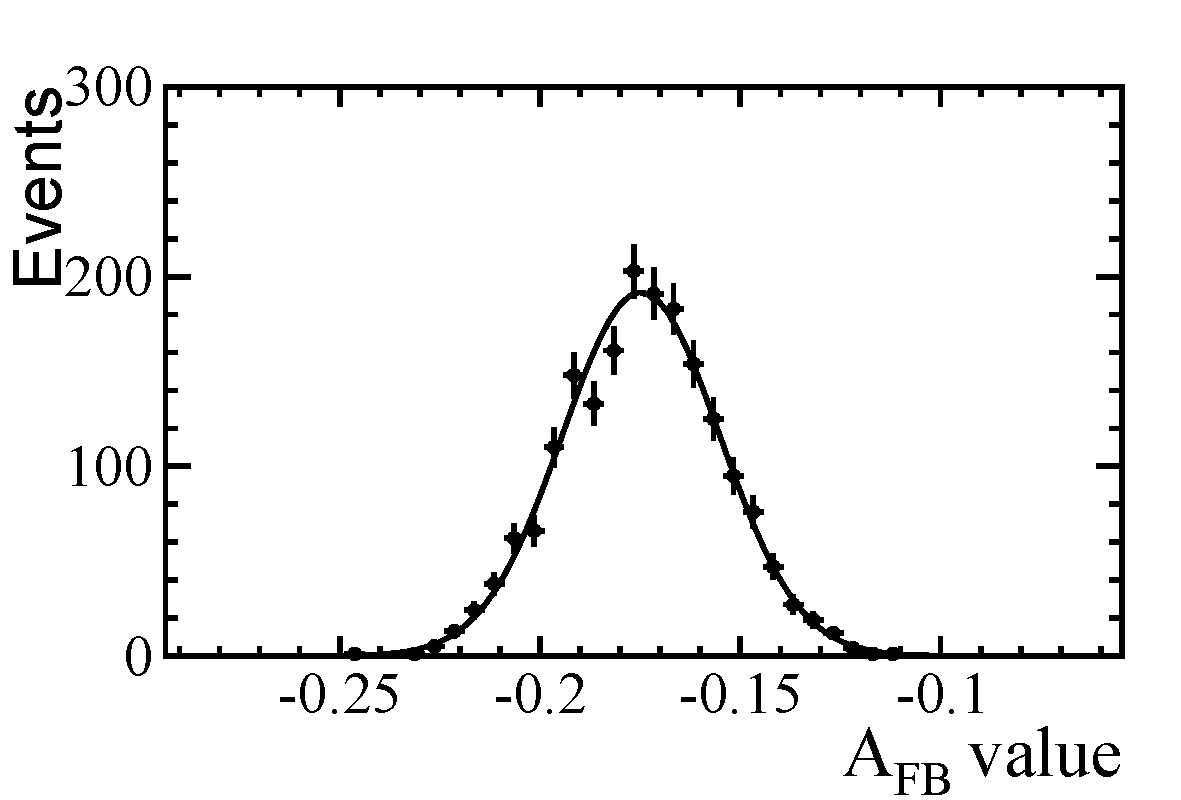
\includegraphics[width=0.48\textwidth]{chapter6/figs/fit_result_test_afb_gen_val_plot_new.pdf}}
\subfigure[]{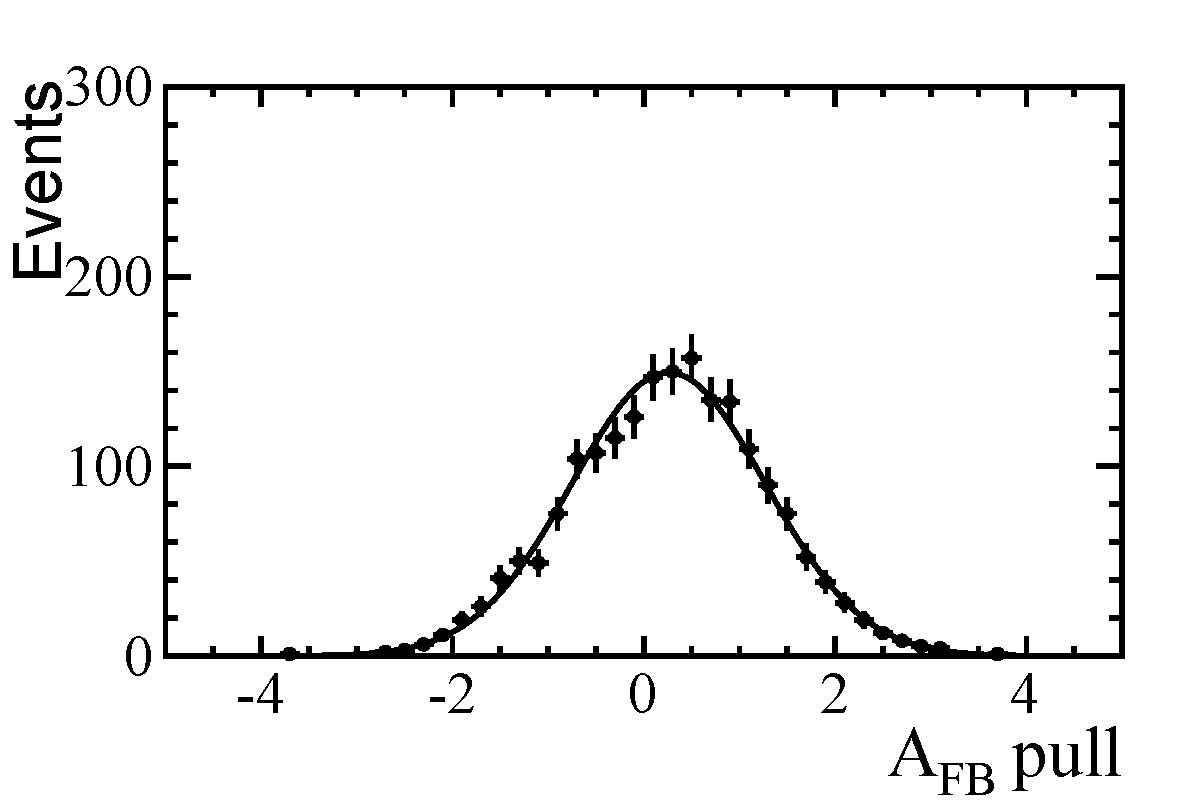
\includegraphics[width=0.48\textwidth]{chapter6/figs/fit_result_test_afb_gen_pull_plot_new.pdf}}
\subfigure[]{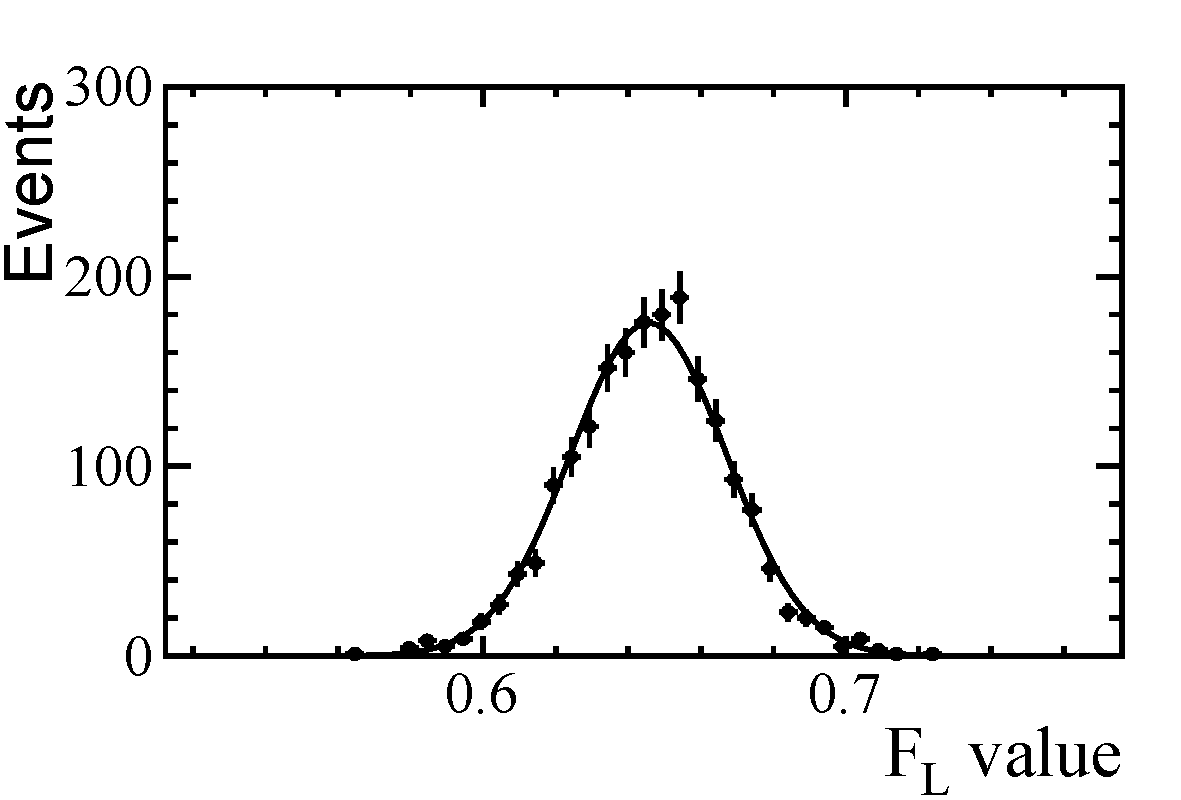
\includegraphics[width=0.48\textwidth]{chapter6/figs/fit_result_test_fl_gen_val_plot_new.pdf}}
\subfigure[]{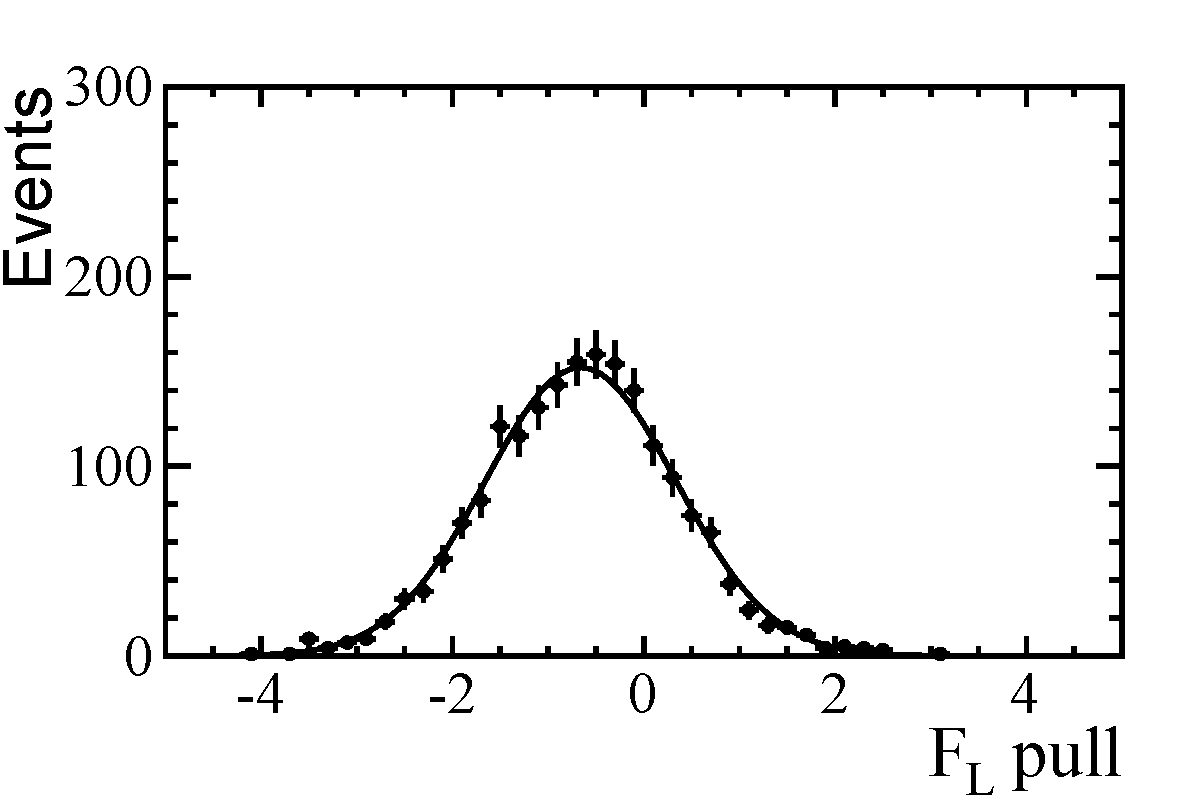
\includegraphics[width=0.48\textwidth]{chapter6/figs/fit_result_test_fl_gen_pull_plot_new.pdf}}
\caption[  Distribution of the results and pull  
values for \AFB (a,b) and \FL (c,d) respectively 
for fits to 1000 toy simulations each containing 1000 events. ]
{Distribution of the results and pull 
values for \AFB (a,b) and \FL (c,d) respectively 
for fits to 1000 toy simulations each containing 1000 events.
The S-wave is ignored in these fits. The resolution obtained on \AFB is 
$0.026\pm0.001$. Since the S-wave is ignored there is a non-zero 
pull mean for both observables at $(0.26\pm0.02)$ and $(-0.65\pm0.02)$ respectively. 
The widths of the pull distribution are consistent with unity at 
 $(1.01\pm0.01)$ and $(0.99\pm0.01)$.~\label{fig:toyexample}}
\end{figure}



\section{The impact of ignoring the S-wave in an angular analysis of \BdToKstll}
\label{sec:swave:ignore}

The effect of ignoring or including a \kpi S-wave was tested as a function of dataset 
 size in order to find a minimum dataset at which the bias 
 from ignoring the S-wave contribution to the angular distribution when measuring the angular observables becomes significant.
Datasets were generated for sample sizes ranging from 50 to 
1000 events and analysed assuming a pure P-wave state. 
The results are shown in Fig.~\ref{fig:bias}. 
\begin{figure}[tb]
\centering
\subfigure[]{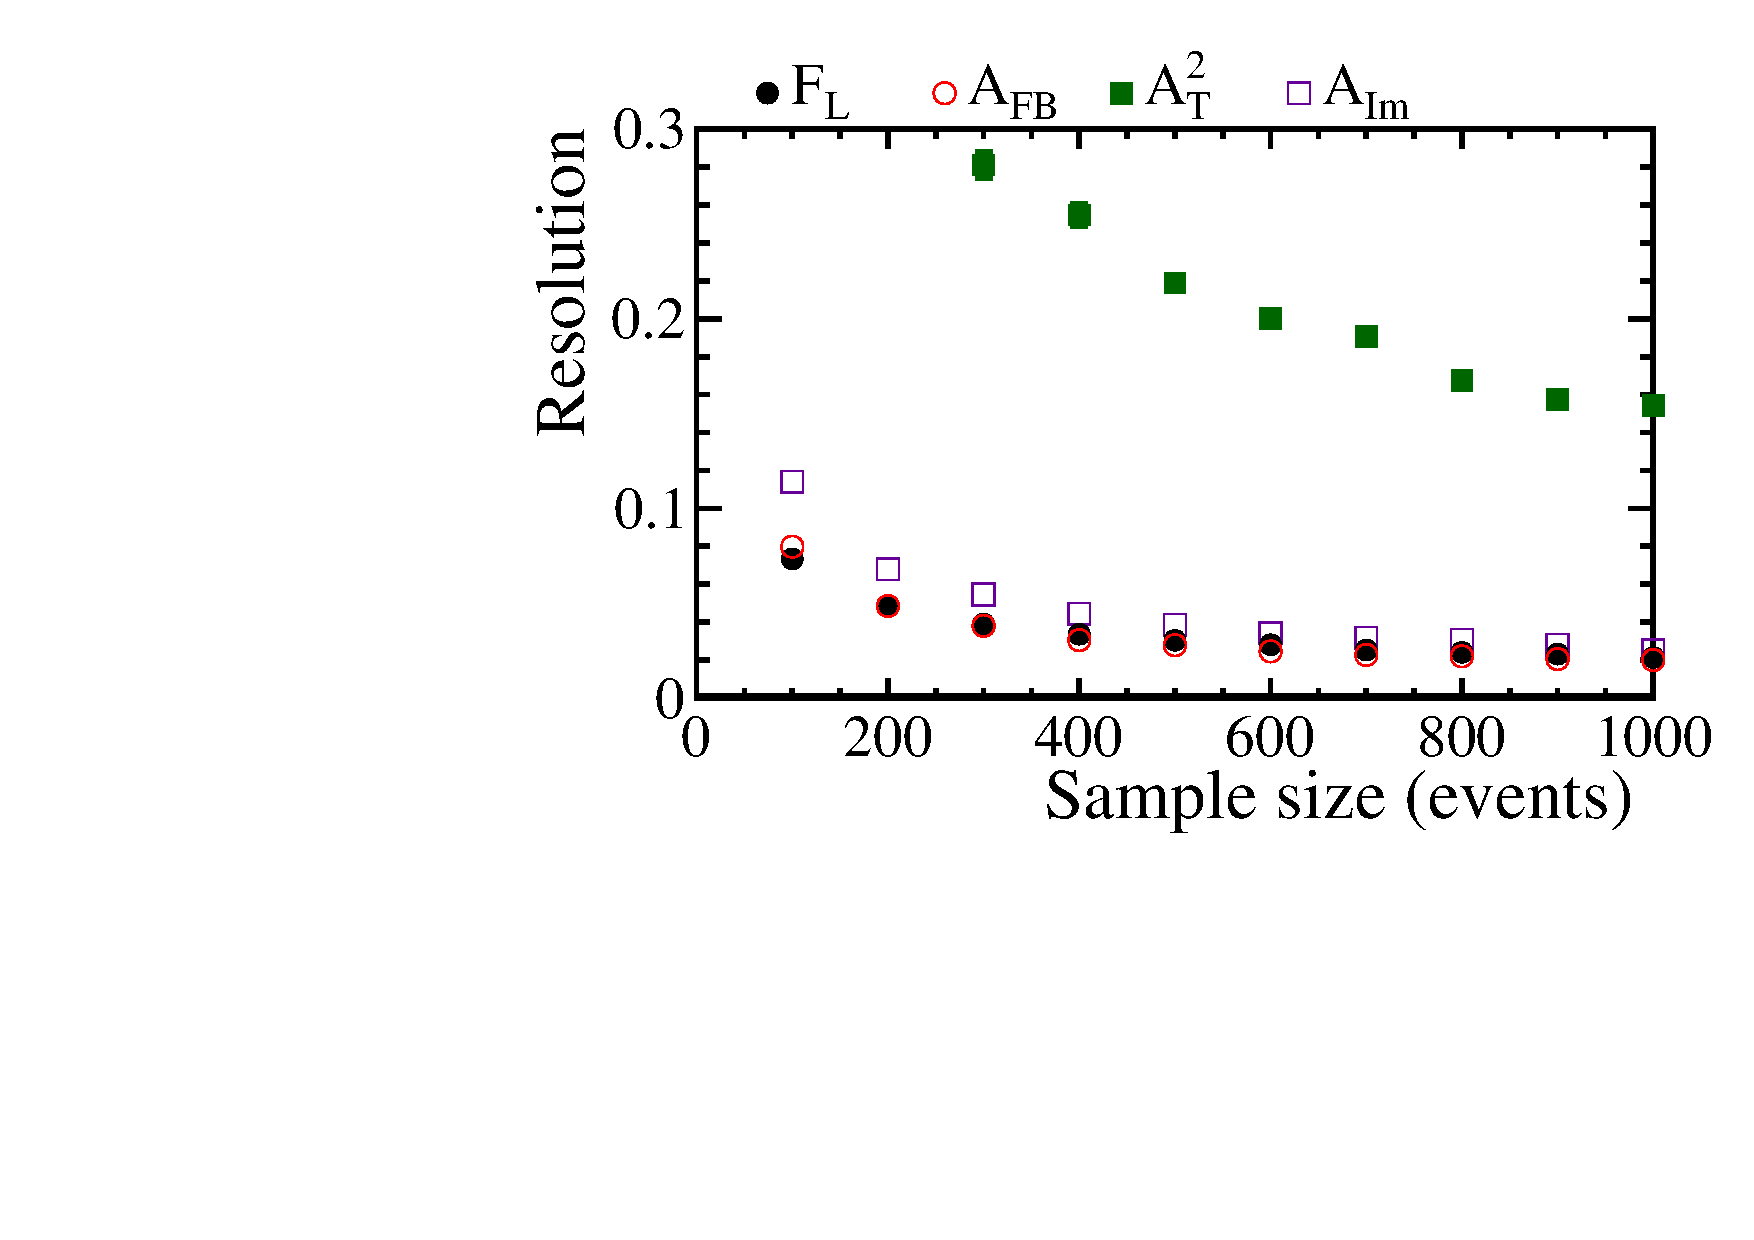
\includegraphics[width=0.48\textwidth]{chapter6/figs/fit_result_ds_gen_res.pdf}}
\subfigure[]{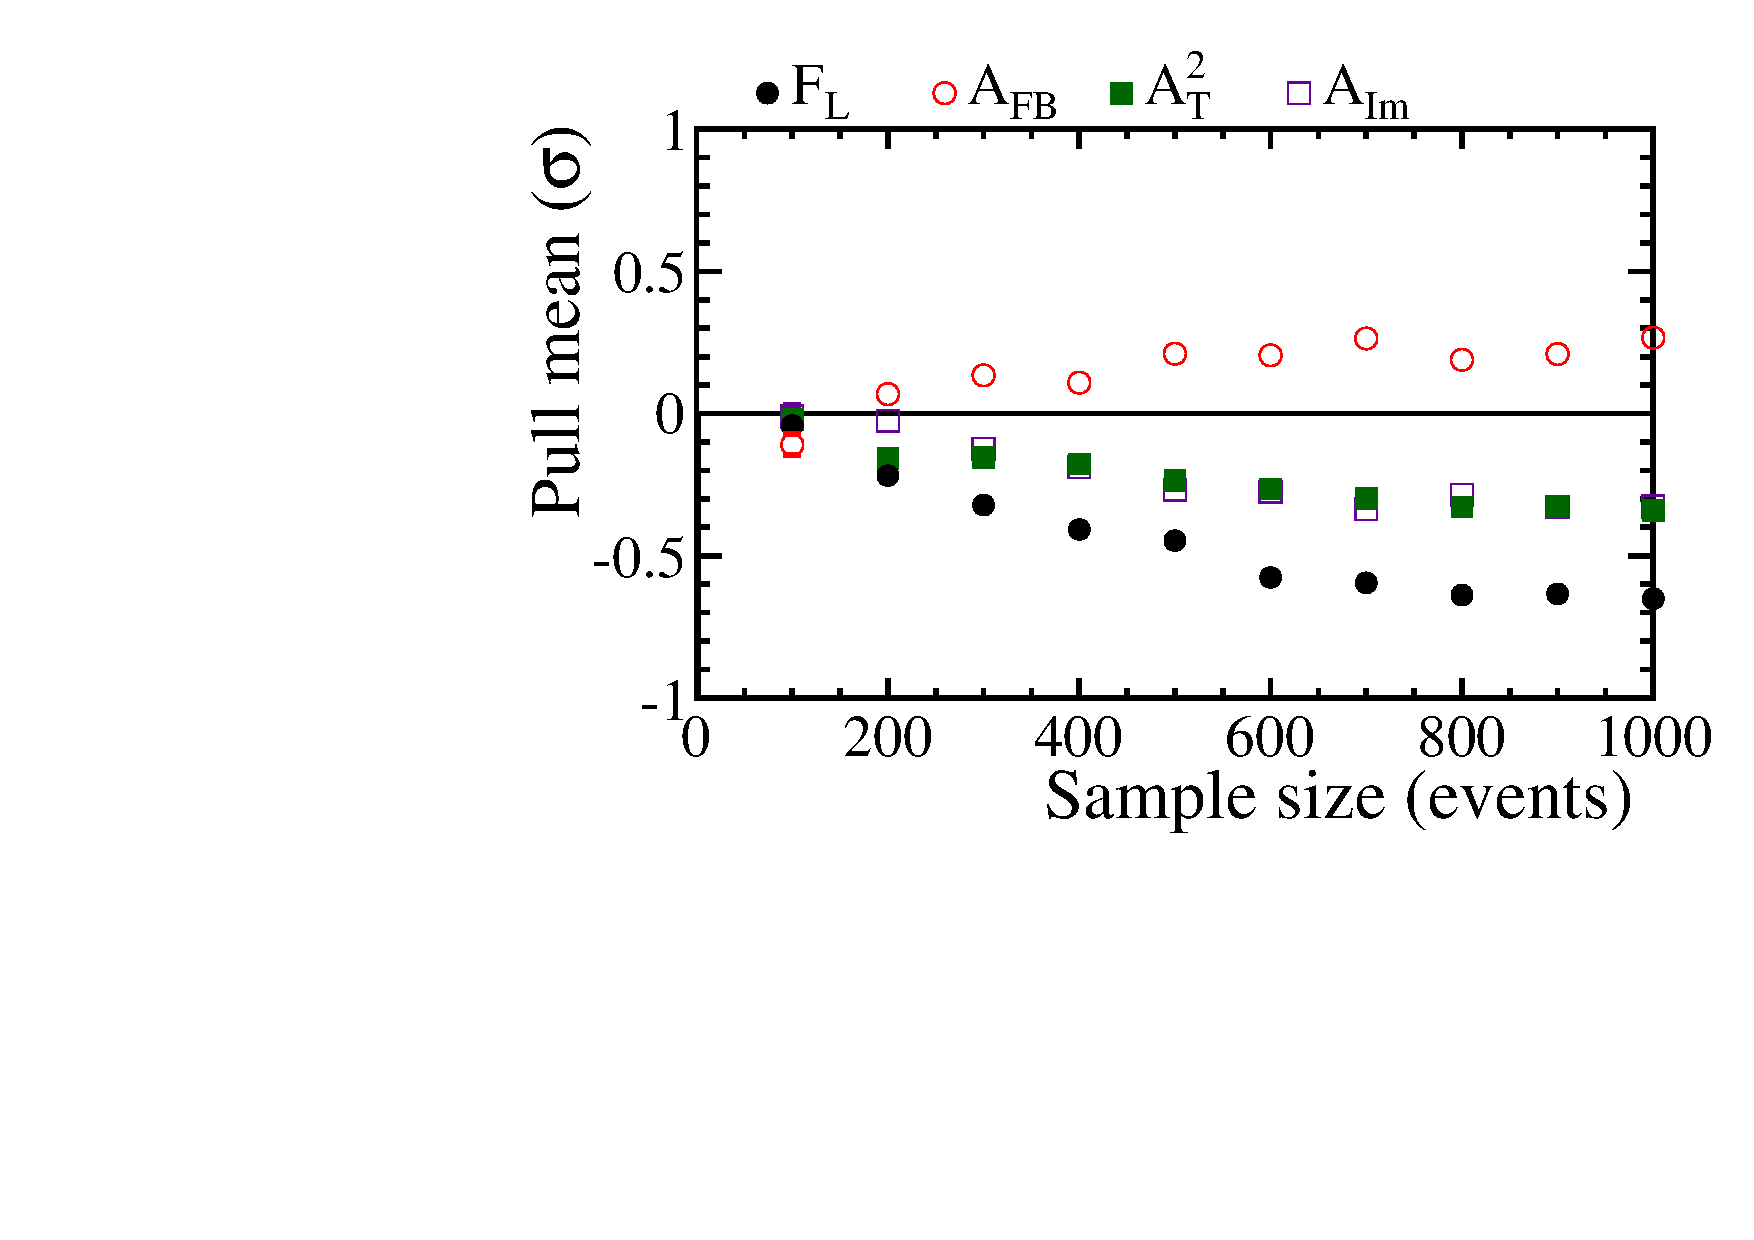
\includegraphics[width=0.48\textwidth]{chapter6/figs/fit_result_ds_gen_mean.pdf}}
\subfigure[]{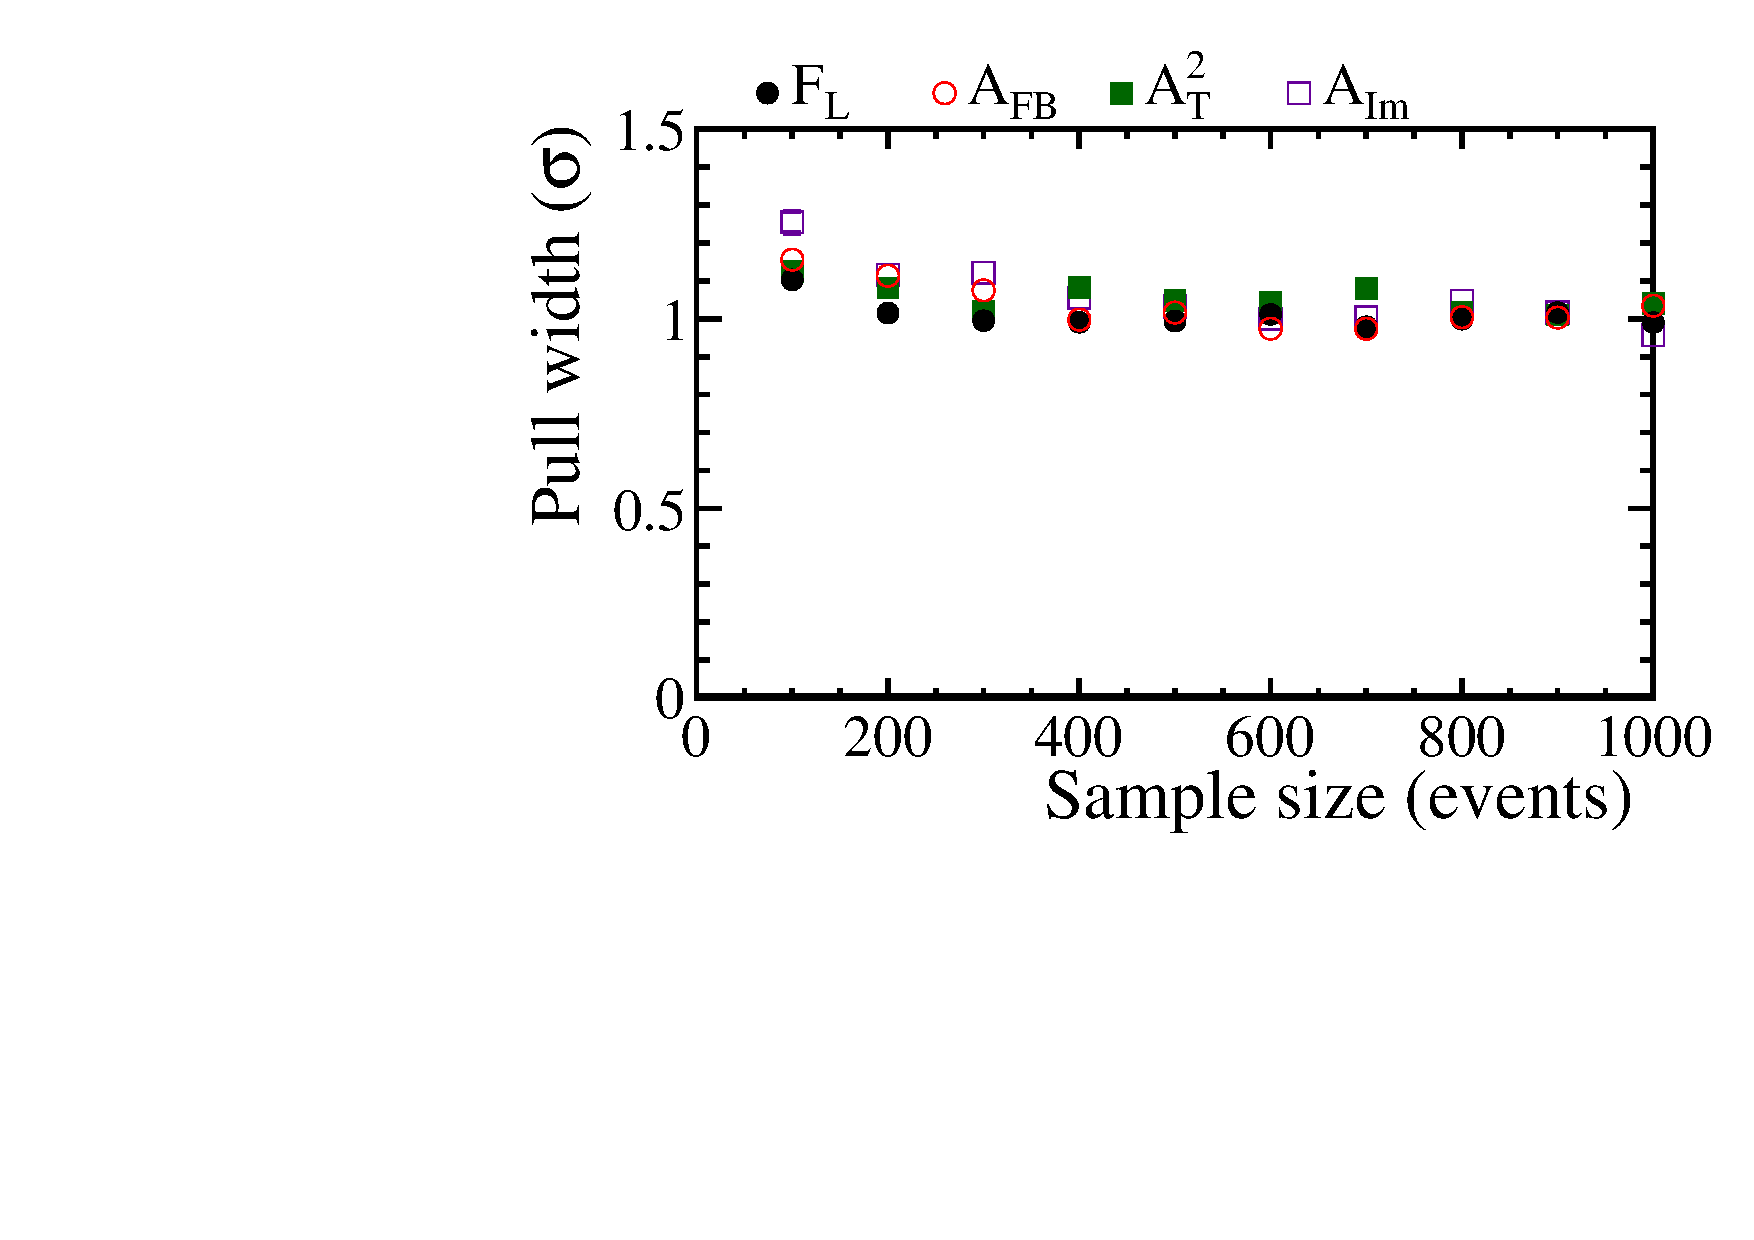
\includegraphics[width=0.48\textwidth]{chapter6/figs/fit_result_ds_gen_width.pdf}}
\caption[ Resolution, pull mean and width of 
1000 toy datasets analysed as a pure P-wave state as a 
function of dataset size.    ]
{Resolution (a), pull mean (b) and pull width (c) of 
1000 toy datasets analysed as a pure P-wave state as a 
function of dataset size. It can be seen that the bias 
on the observable (non-zero pull mean) increases dramatically as the sample 
size increases. This is because the statistical error 
decreases increasing the sensitivity to the ignored S-wave 
contribution. The bias of \AFB is positive  
because \AFB is negative in the \qsq bin chosen. 
~\label{fig:bias}}
\end{figure}

From Eq.~\ref{eq:theo4d}, it can be seen that \AT2 
has a factor of (1-\FL) in front of it. The large 
value of \FL used to generated datasets is 
in turn causing \AT2 to have a much worse 
resolution than \AFB, \FL and \OS3 . There is 
significant bias (non-zero mean) of the pull distribution for all
 observables when the S-wave is ignored in the angular distribution for datasets 
 of more than 200 events. This corresponds to a 
 change of 0.2$\sigma$ in \FL for a dataset of 200 events.
The behaviour can be understood in terms of the $(1-\FS)$ 
factor in Eq.~\ref{eq:theo4d}. It gives an offset to the 
fitted values of the observables which are proportional 
to the value of $(1-\FS)$.

The angular fit was performed on toy 
datasets with an increasing S-wave contribution.
Datasets of 500 events were generated with a 
varying S-wave contribution in the narrow \psq
 mass window of ($800 < p < 1000 \mev$) 
 from no S-wave up to a \FS value of $0.4$. 
The resolution and the mean and width of the pull 
distribution for each of the four observables
 (\AFB, \FL, \AT2 , \OS3 ) were calculated and 
 the results are shown in Fig.~\ref{fig:fsval}.
\begin{figure}[tb]
\centering
\subfigure[]{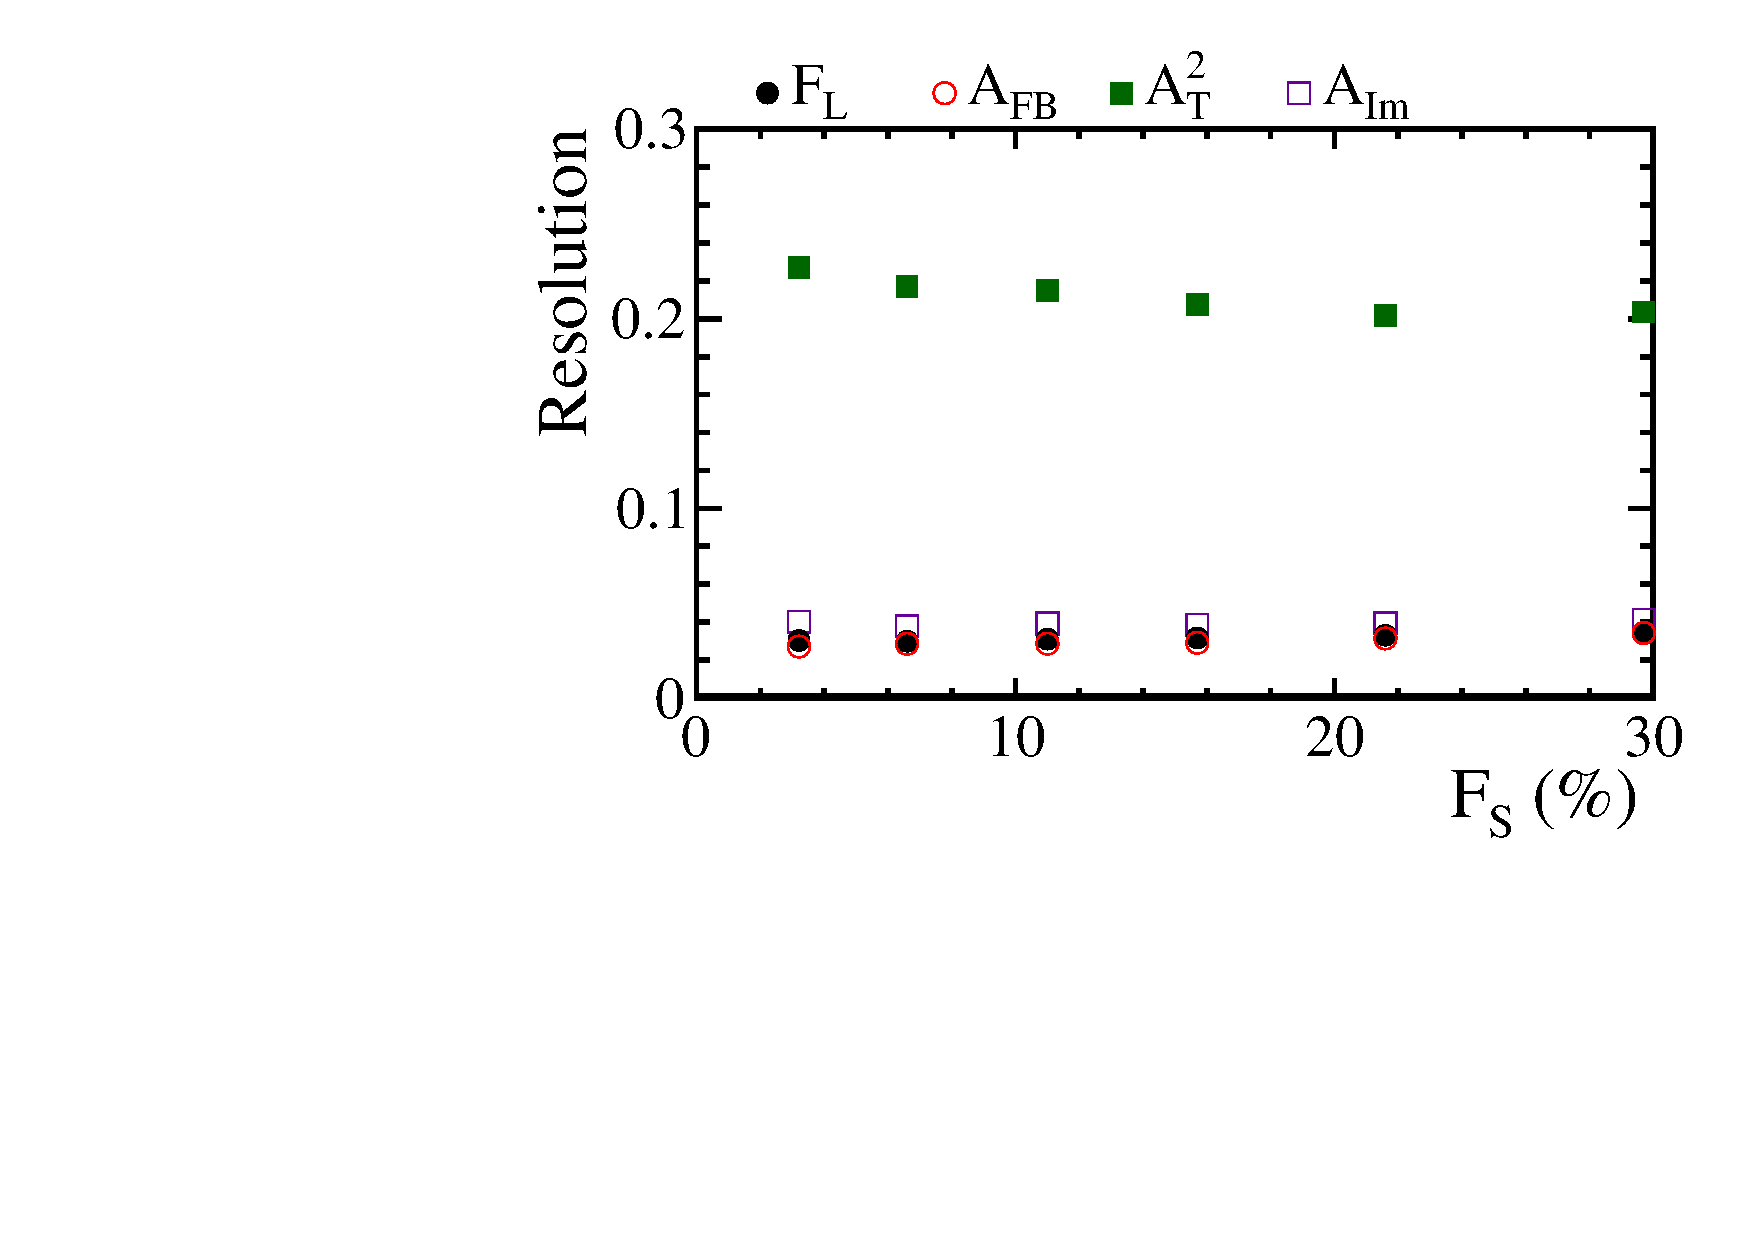
\includegraphics[width=0.48\textwidth]{chapter6/figs/fit_result_fs_gen_res.pdf}}
\subfigure[]{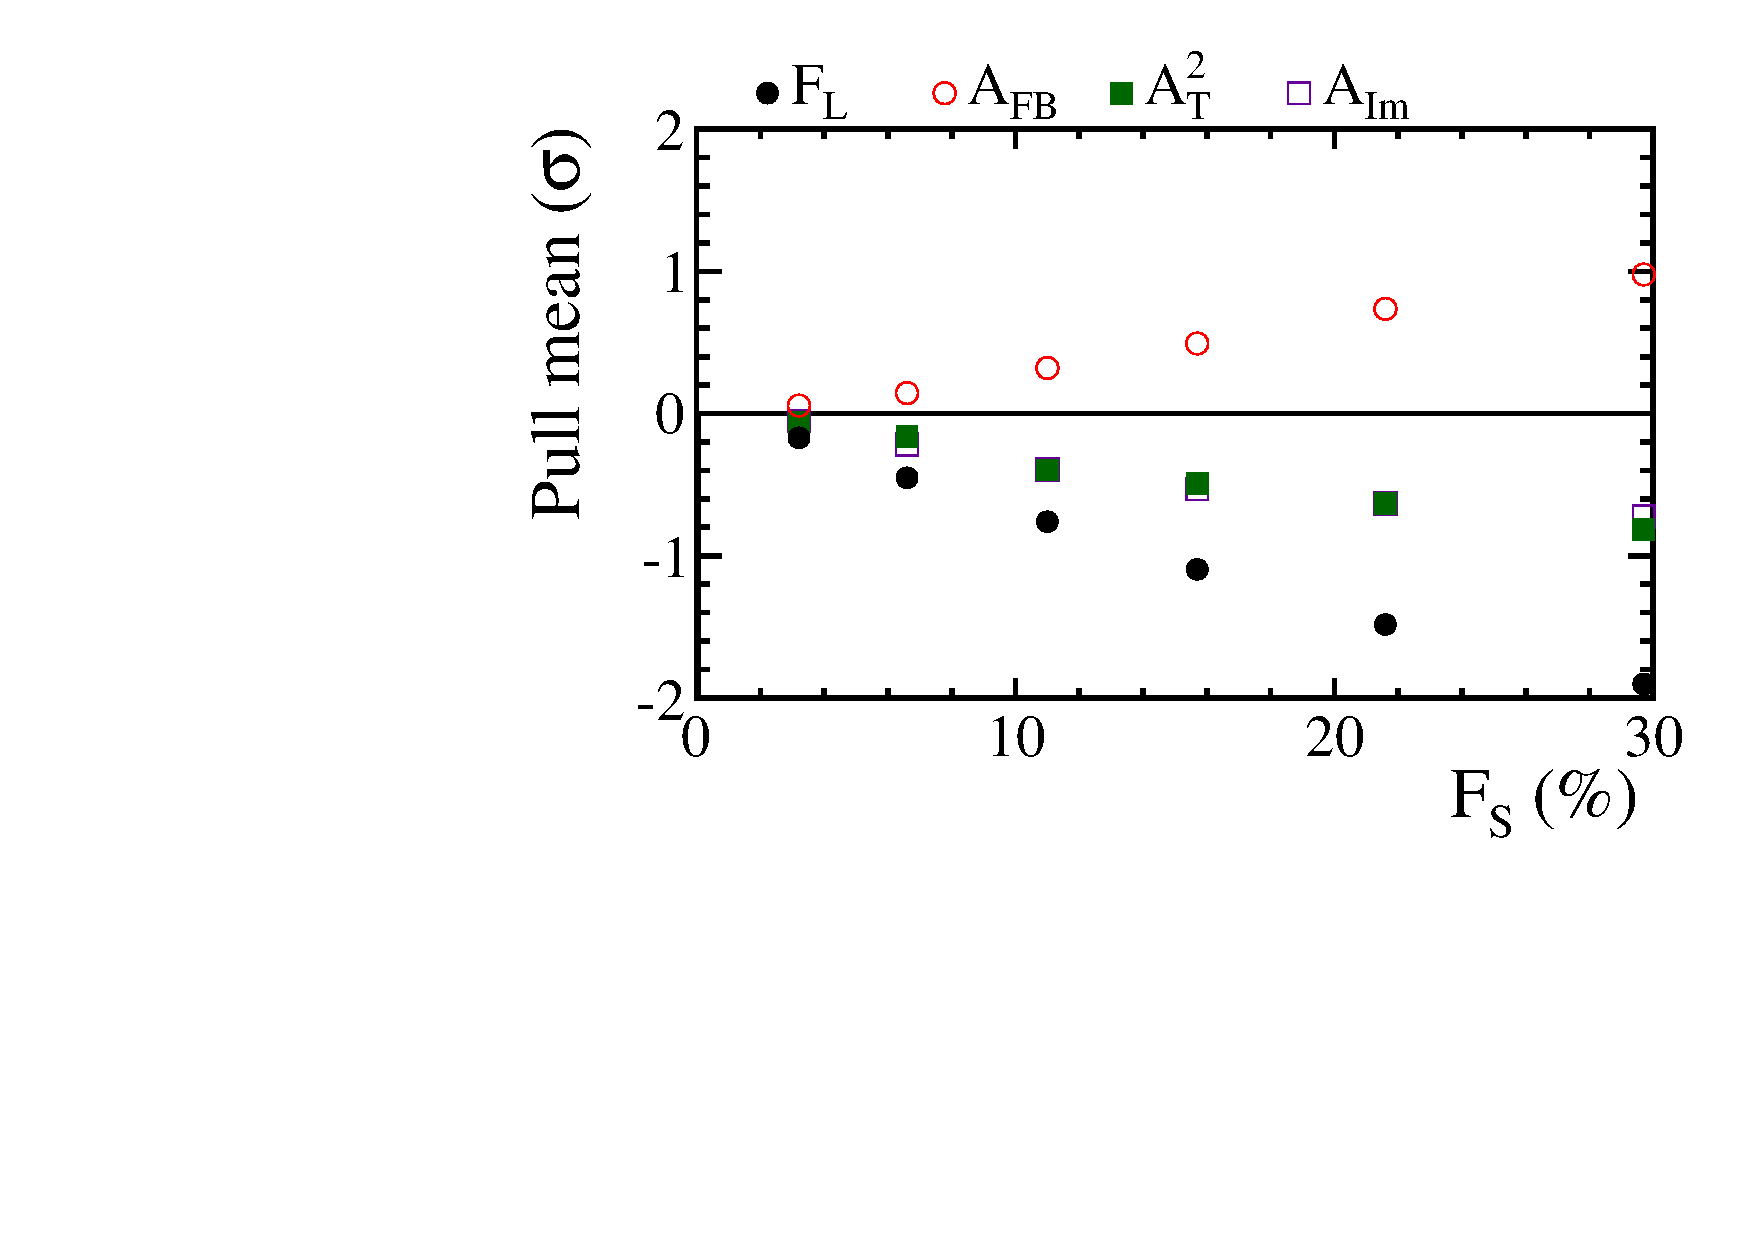
\includegraphics[width=0.48\textwidth]{chapter6/figs/fit_result_fs_gen_mean.pdf}}
\subfigure[]{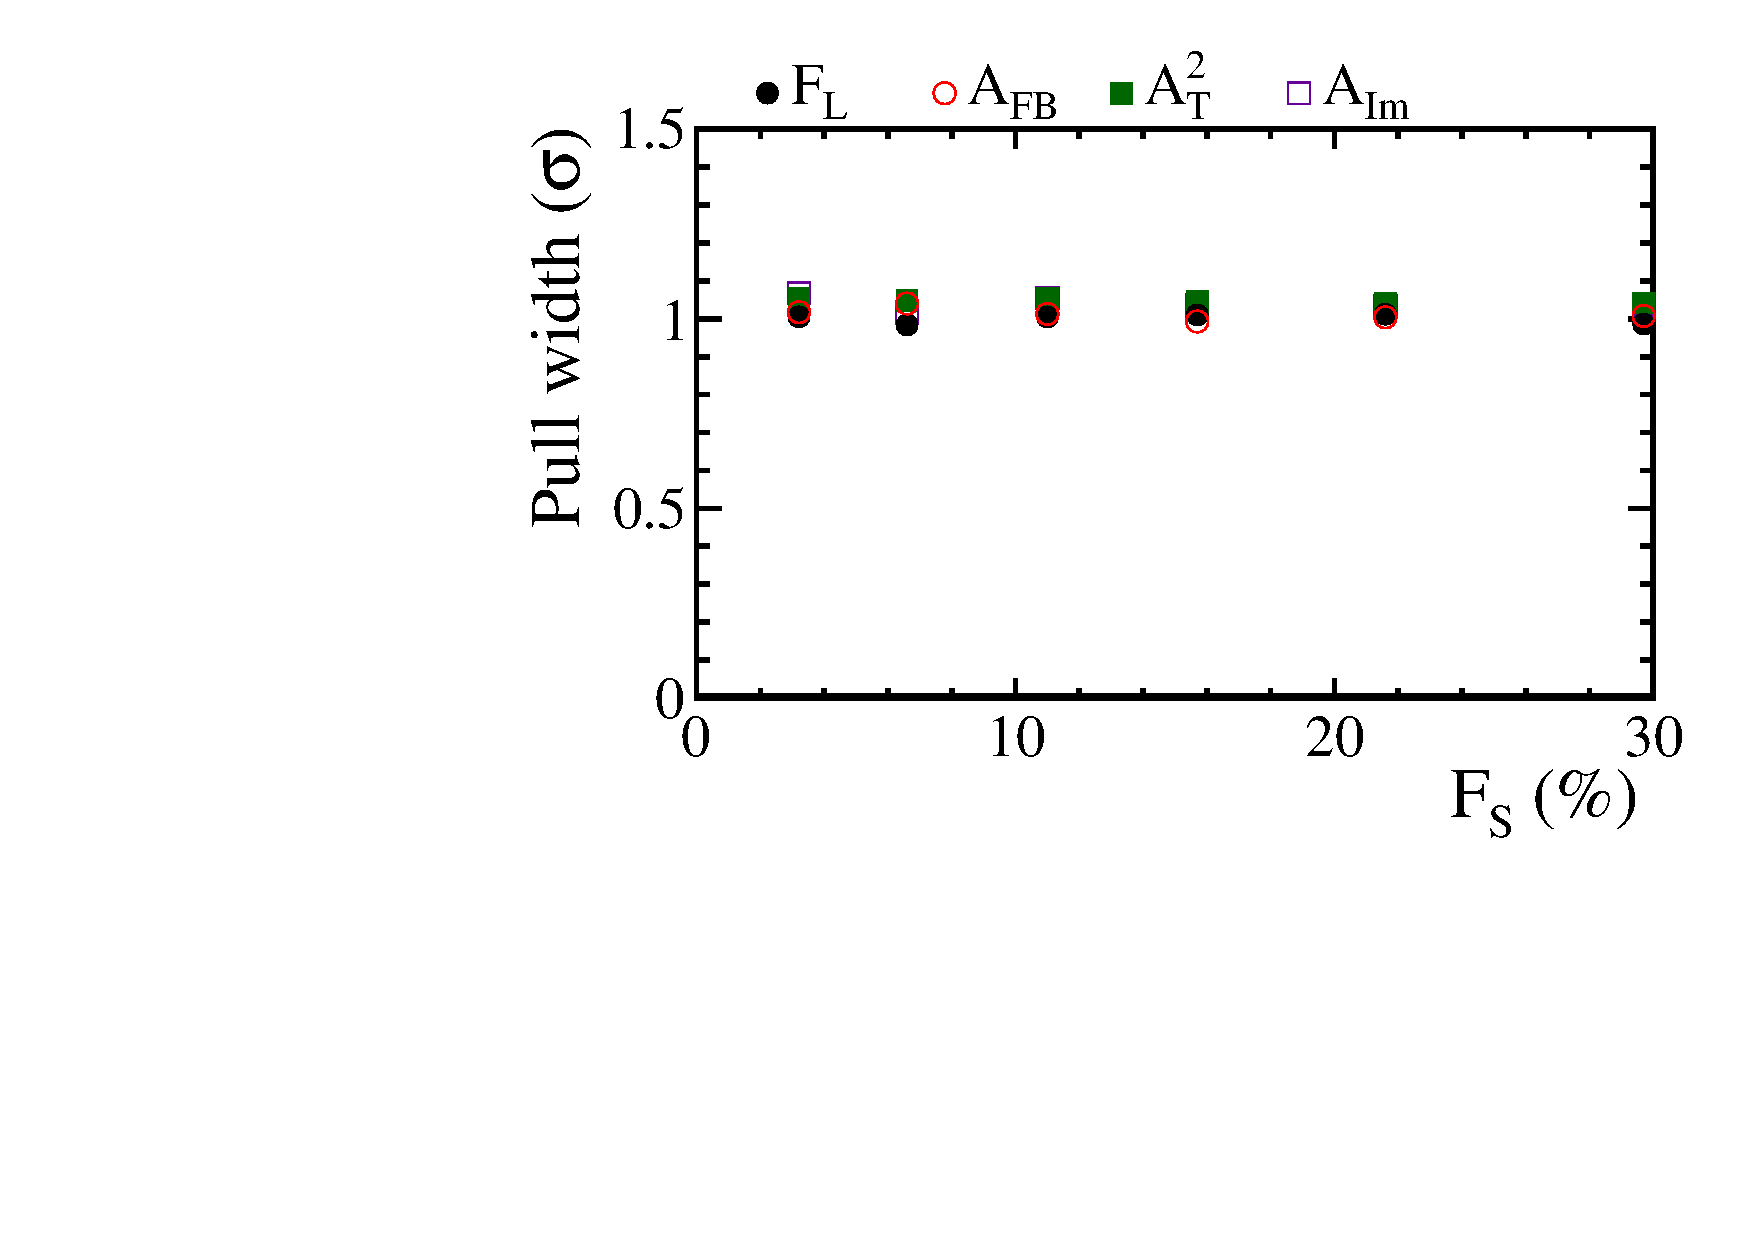
\includegraphics[width=0.48\textwidth]{chapter6/figs/fit_result_fs_gen_width.pdf}}
\caption[ The resolution, mean and width of the pull distribution 
of 1000 toy datasets analysed as a pure 
P-wave state as a function of the S-wave contribution.   ]
{The resolution (a) the mean (b) and the width (c) of the pull distribution
of 1000 toy datasets analysed as a pure 
P-wave state as a function of S-wave contribution. 
The resolution and the bias can be seen to increase with the size of the S-wave 
contribution in a linear fashion. ~\label{fig:fsval}}
\end{figure}
Significant bias is seen in the angular 
observables when the S-wave is ignored for an S-wave magnitude of greater than 5\%.
The linear increase in the bias 
is another consequence of the (1-\FS) factor in the angular distribution.



\section{Measuring the S-wave in \BdToKpill}
\label{sec:swave:measurement}

Obtaining unbiased values for the angular observables beyond the limits
 shown requires including the S-wave contribution in the angular model. % rather than ignoring it.
With the formalism developed in Section~\ref{sec:swave:theo}, three options are explored for measuring
it. The first option is to ignore the \psq dependence in the measured parameters and simply fit for
\psq-averaged values of \FS and \AS. The second option is to fit the \psq 
 line-shape simultaneously with the angular distribution.
This can be done in a small $p$ window between $800$ and $1000\mev$
or in the region from the lower kinematic threshold 
to $1200\mev$.
In all cases the datasets used to perform the 
studies are identical to those used in Sect. 5.1 
%The difference is in how the fit is performed.In each case, 
and the dataset and the S-wave sizes 
refer to the number of events in the smaller \psq window.

The angular distribution without \psq dependence is given in Eq.~\ref{eq:theo4dint}.
For each set of samples, the resolution and the mean 
and the width of the pull distribution of the angular observables are tested. 

The change in the resolution obtained on the angular observables 
for the three different methods of including the S-wave in the angular distribution
 (ignoring the \psq dependence, fitting a narrow \psq window and fitting a wide \psq window) 
is demonstrated by plotting the ratio with respect
to the resolution obtained when a single 
P-wave state is assumed.

The resolution and the mean of the pull distributions for the three different fit methods are shown
relative to the resolution and mean obtained using the assumption of a pure P-wave state. 
The ratio between the fit methods, including the S-wave in the angular distribution and 
assuming a P-wave state, as a function of dataset size
are shown in  Fig~\ref{fig:ratiods}.
\begin{figure}[tb]
\centering
\subfigure[\AFB]{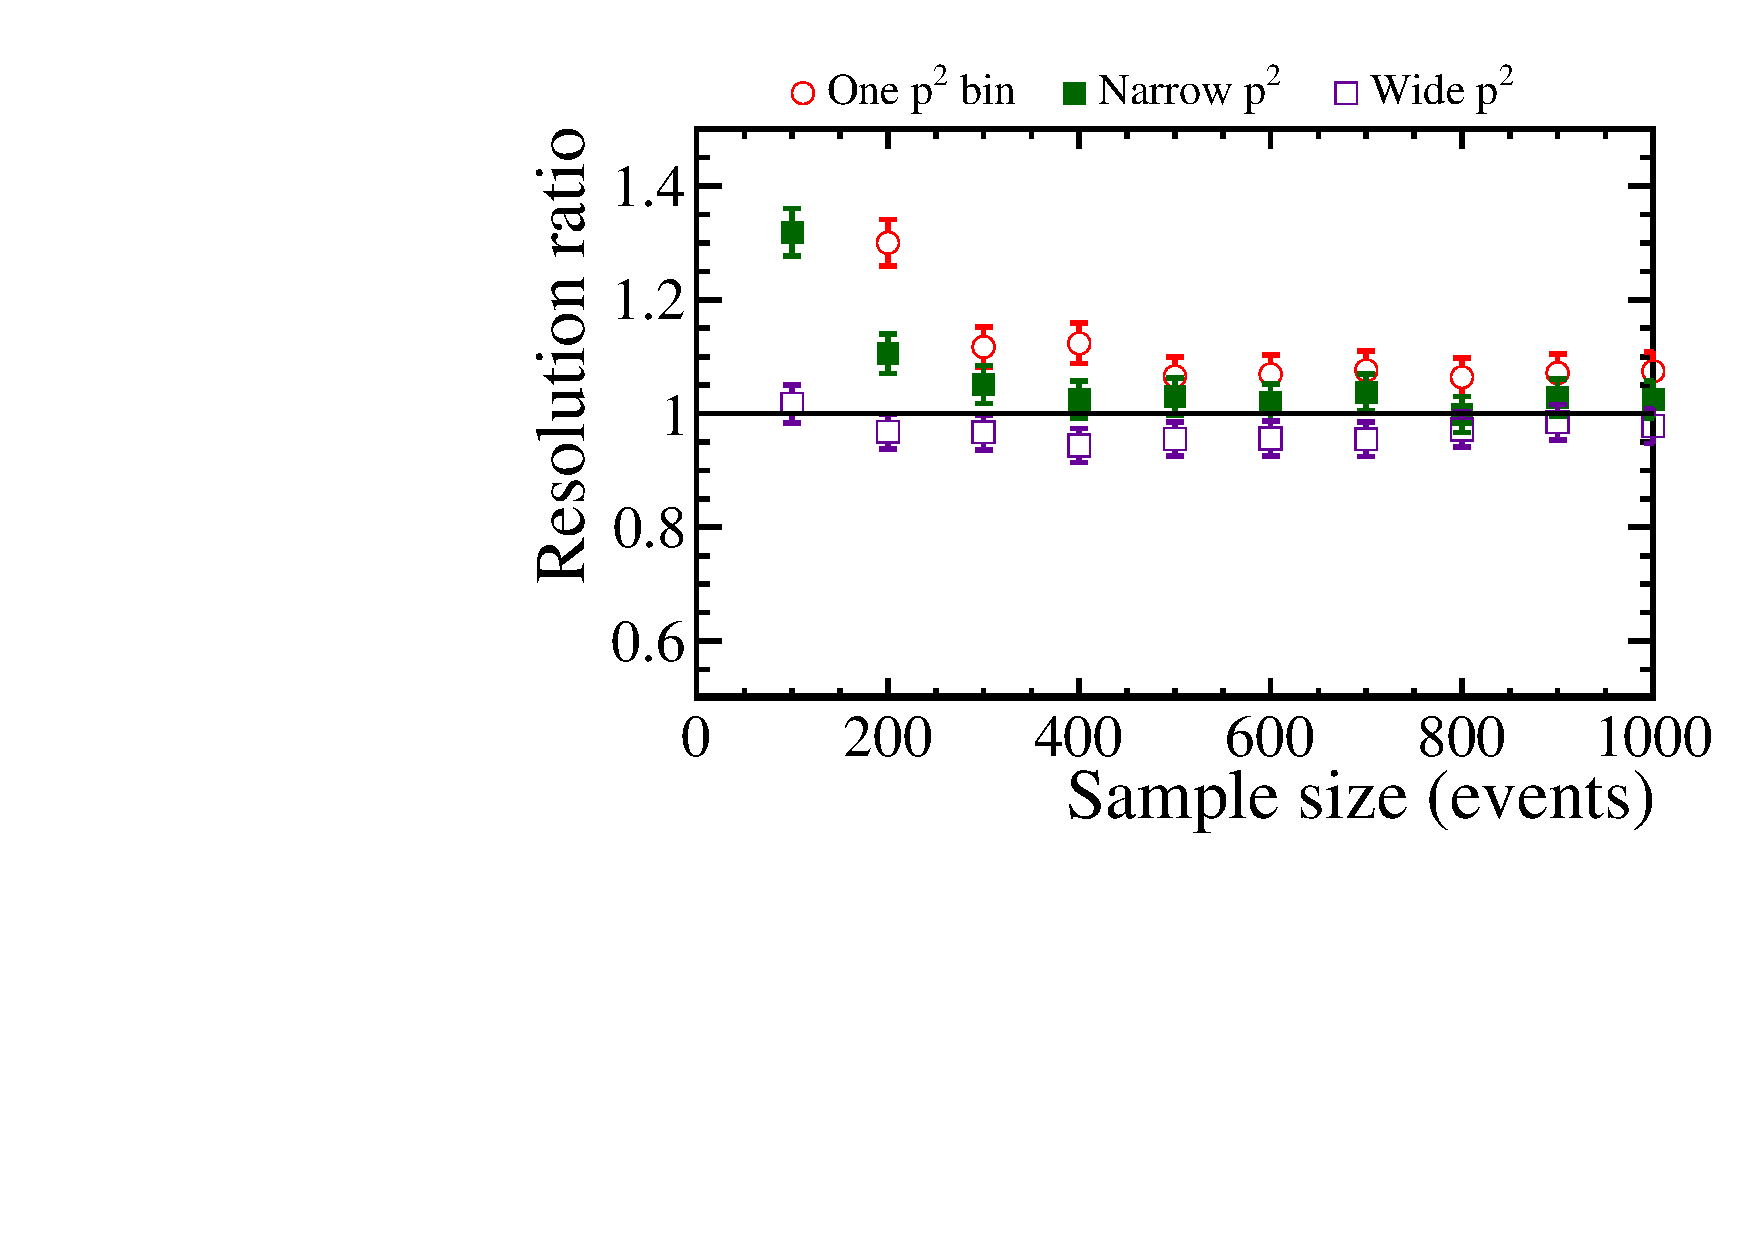
\includegraphics[width=0.48\textwidth]{chapter6/figs/fit_result_ratio_ds_afb_res.pdf}}
\subfigure[\FL]{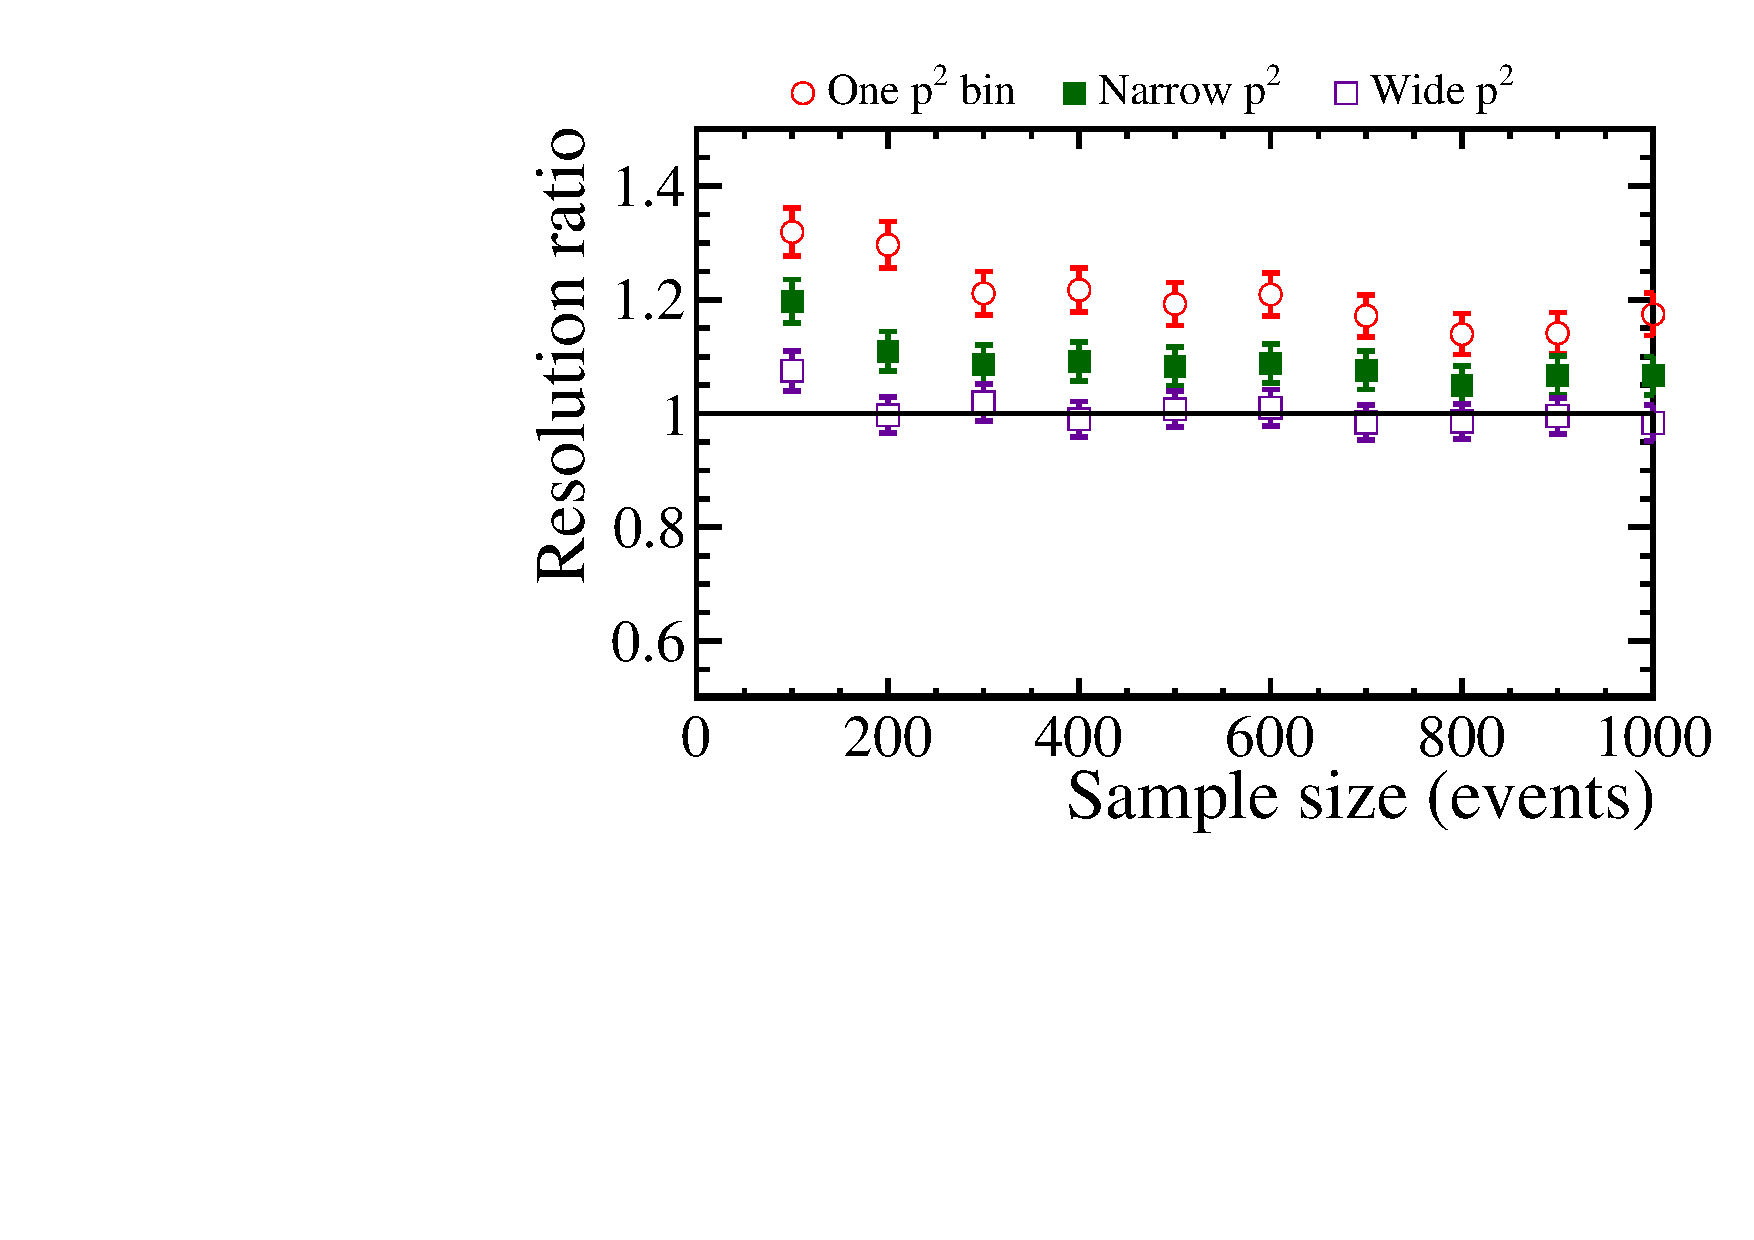
\includegraphics[width=0.48\textwidth]{chapter6/figs/fit_result_ratio_ds_fl_res.pdf}}
\subfigure[\AT2 ]{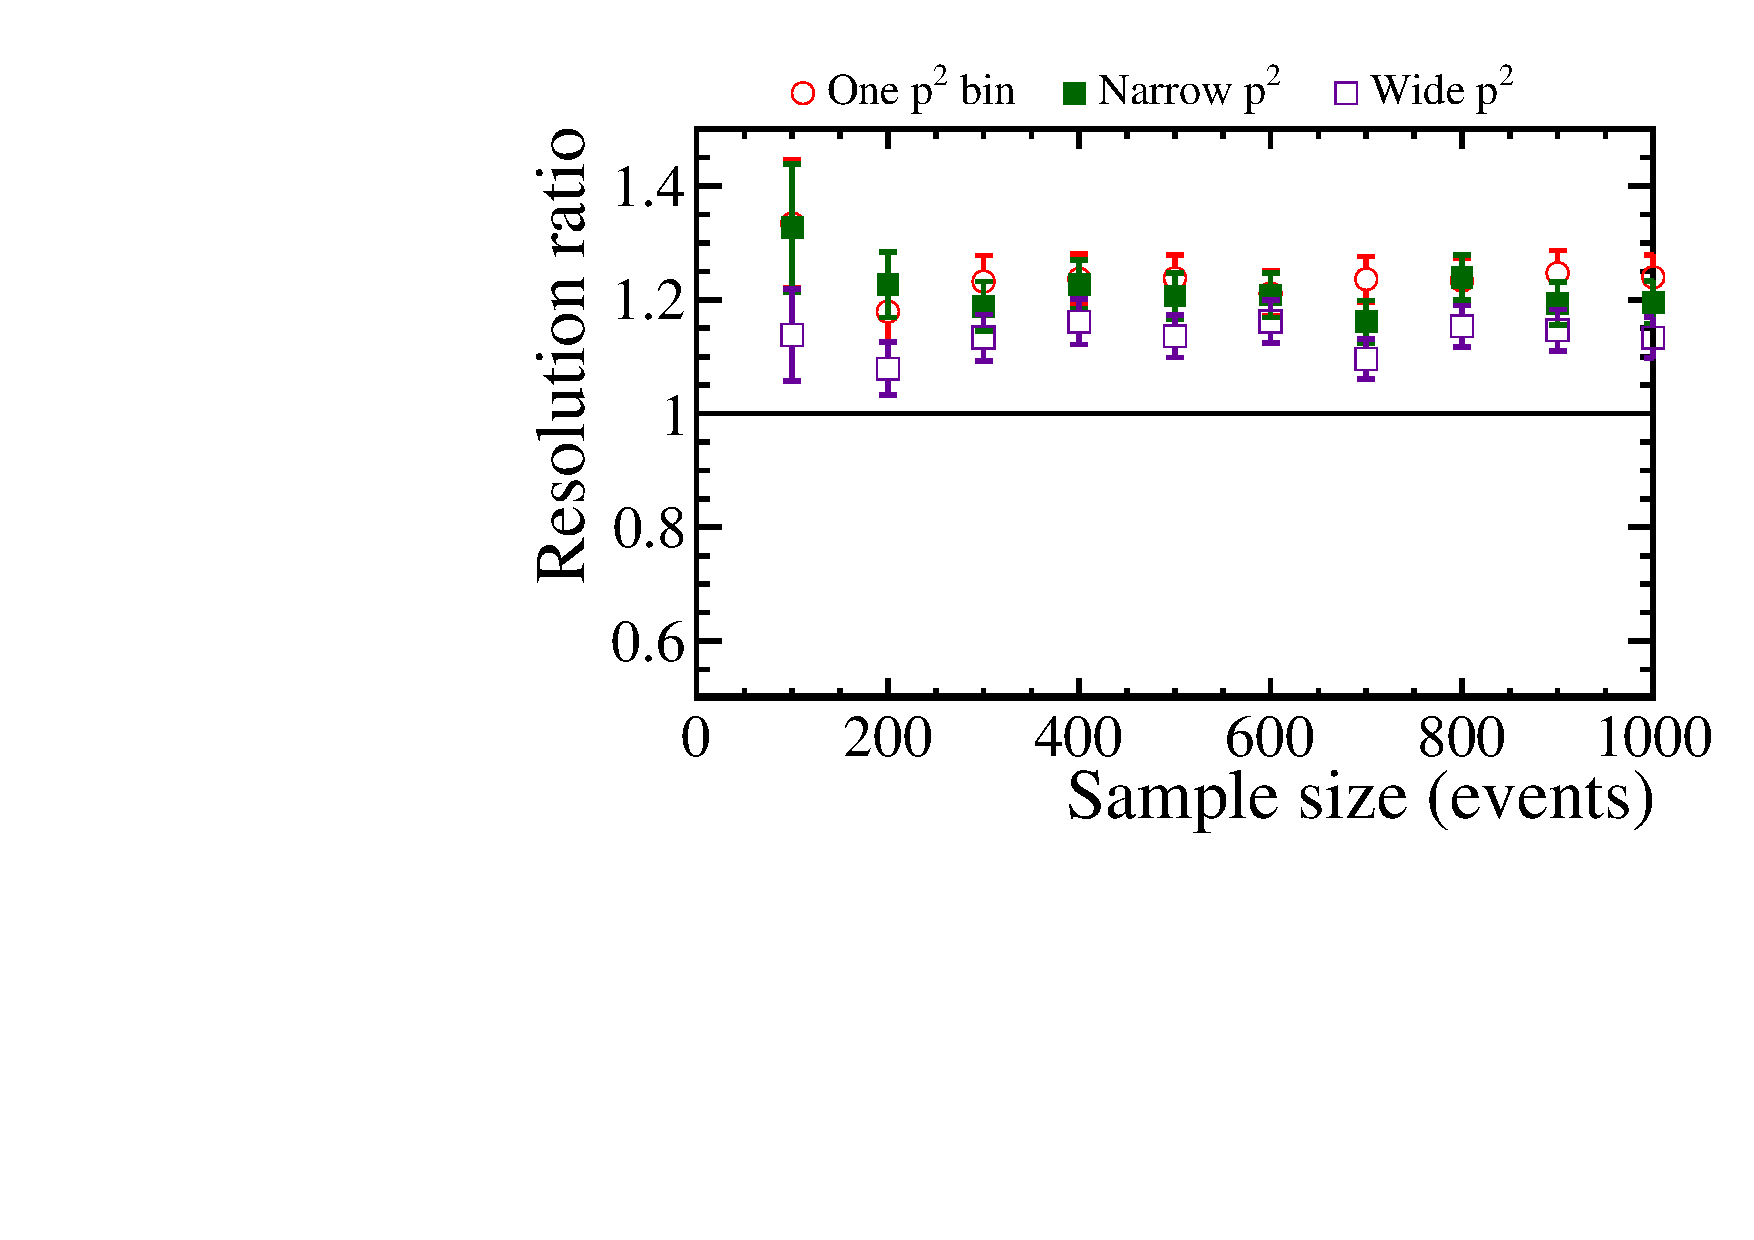
\includegraphics[width=0.48\textwidth]{chapter6/figs/fit_result_ratio_ds_at2_res.pdf}}
\subfigure[\AIm]{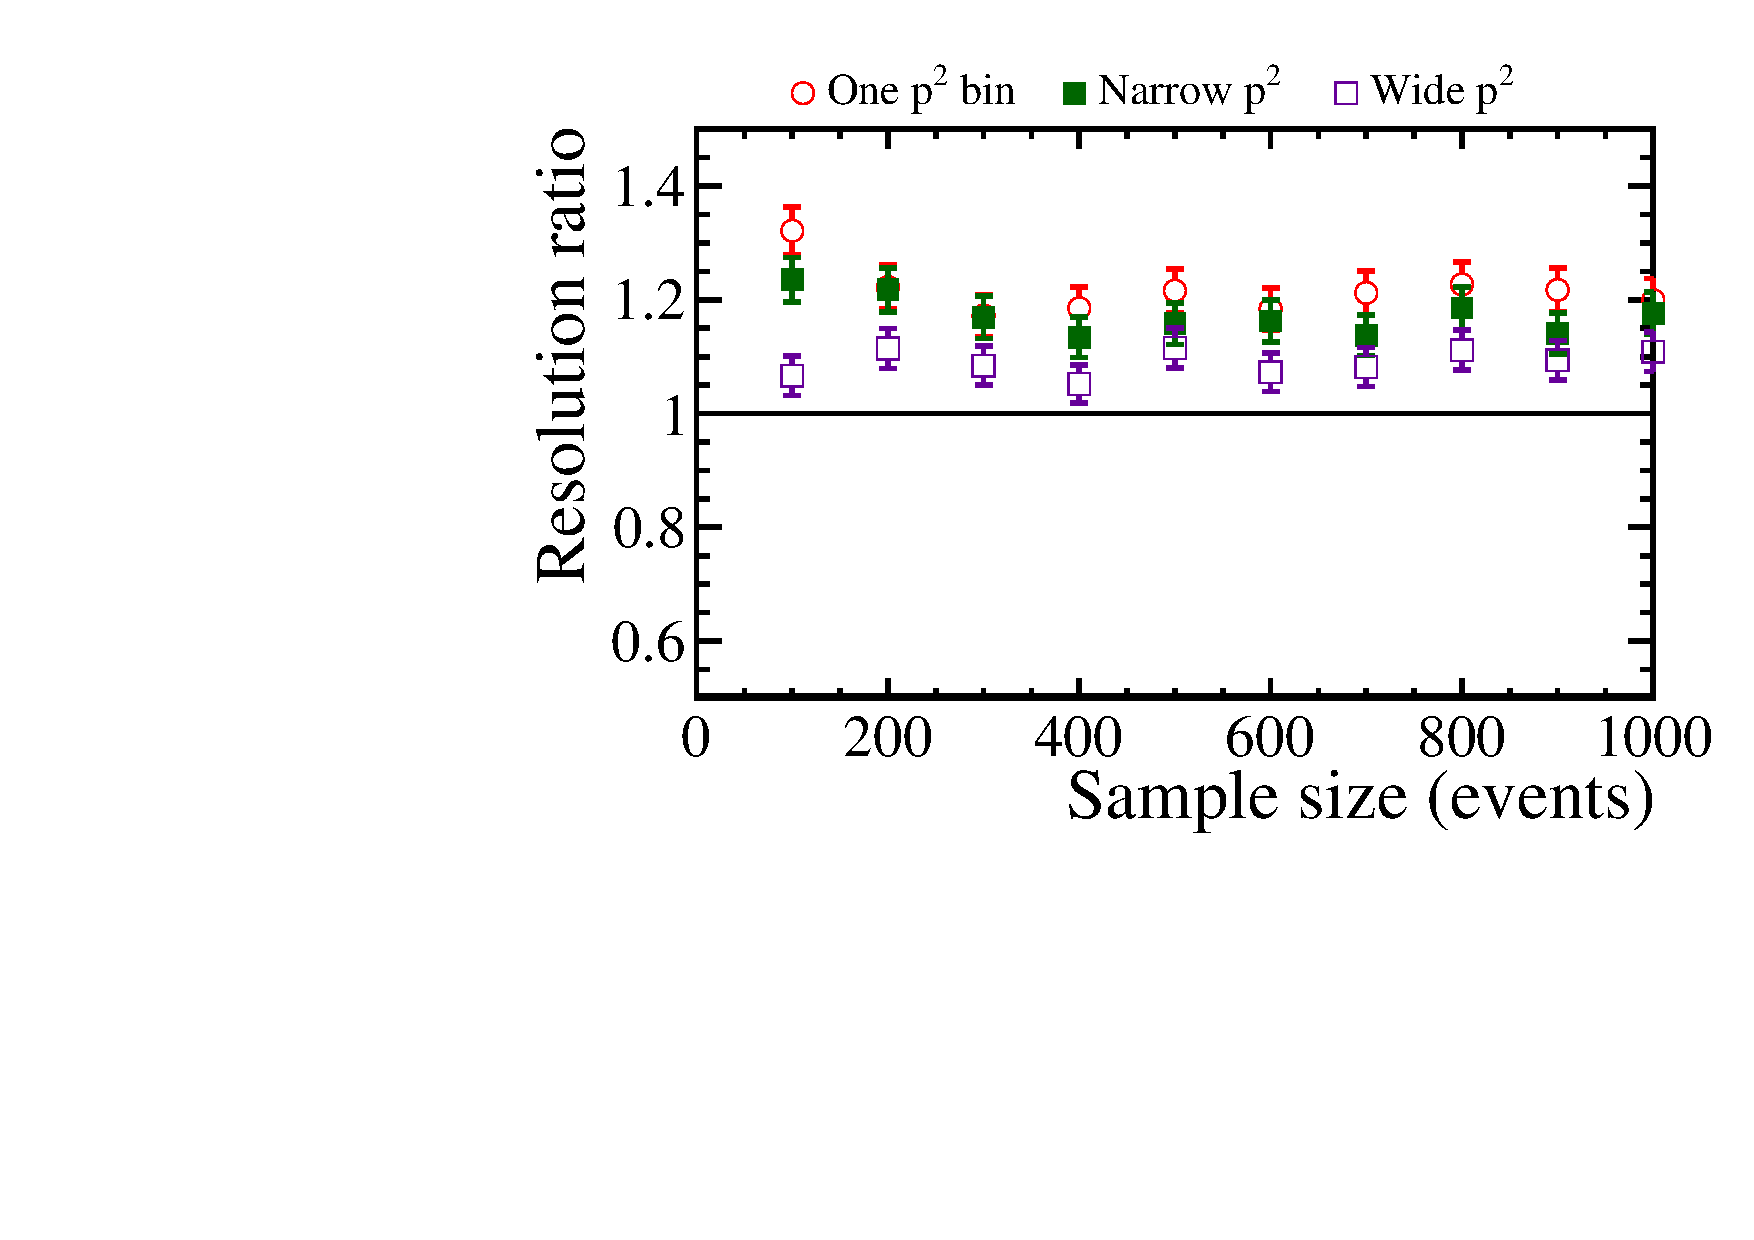
\includegraphics[width=0.48\textwidth]{chapter6/figs/fit_result_ratio_ds_aim_res.pdf}}
\caption[ Resolutions for three different methods to incorporate 
the S-wave relative to the resolution obtained when the S-wave is ignored.    ]
{Resolutions for three different methods to incorporate 
the S-wave relative to the resolution obtained when the S-wave is ignored. 
It can be seen that the best resolution is obtained when using the largest \psq window.
The original resolution is recovered to within 10\%. ~\label{fig:ratiods}}
\end{figure}
The pull mean for all three fit methods is shown in Fig~\ref{fig:combods}.
\begin{figure}[tb]
\centering
\subfigure[\AFB]{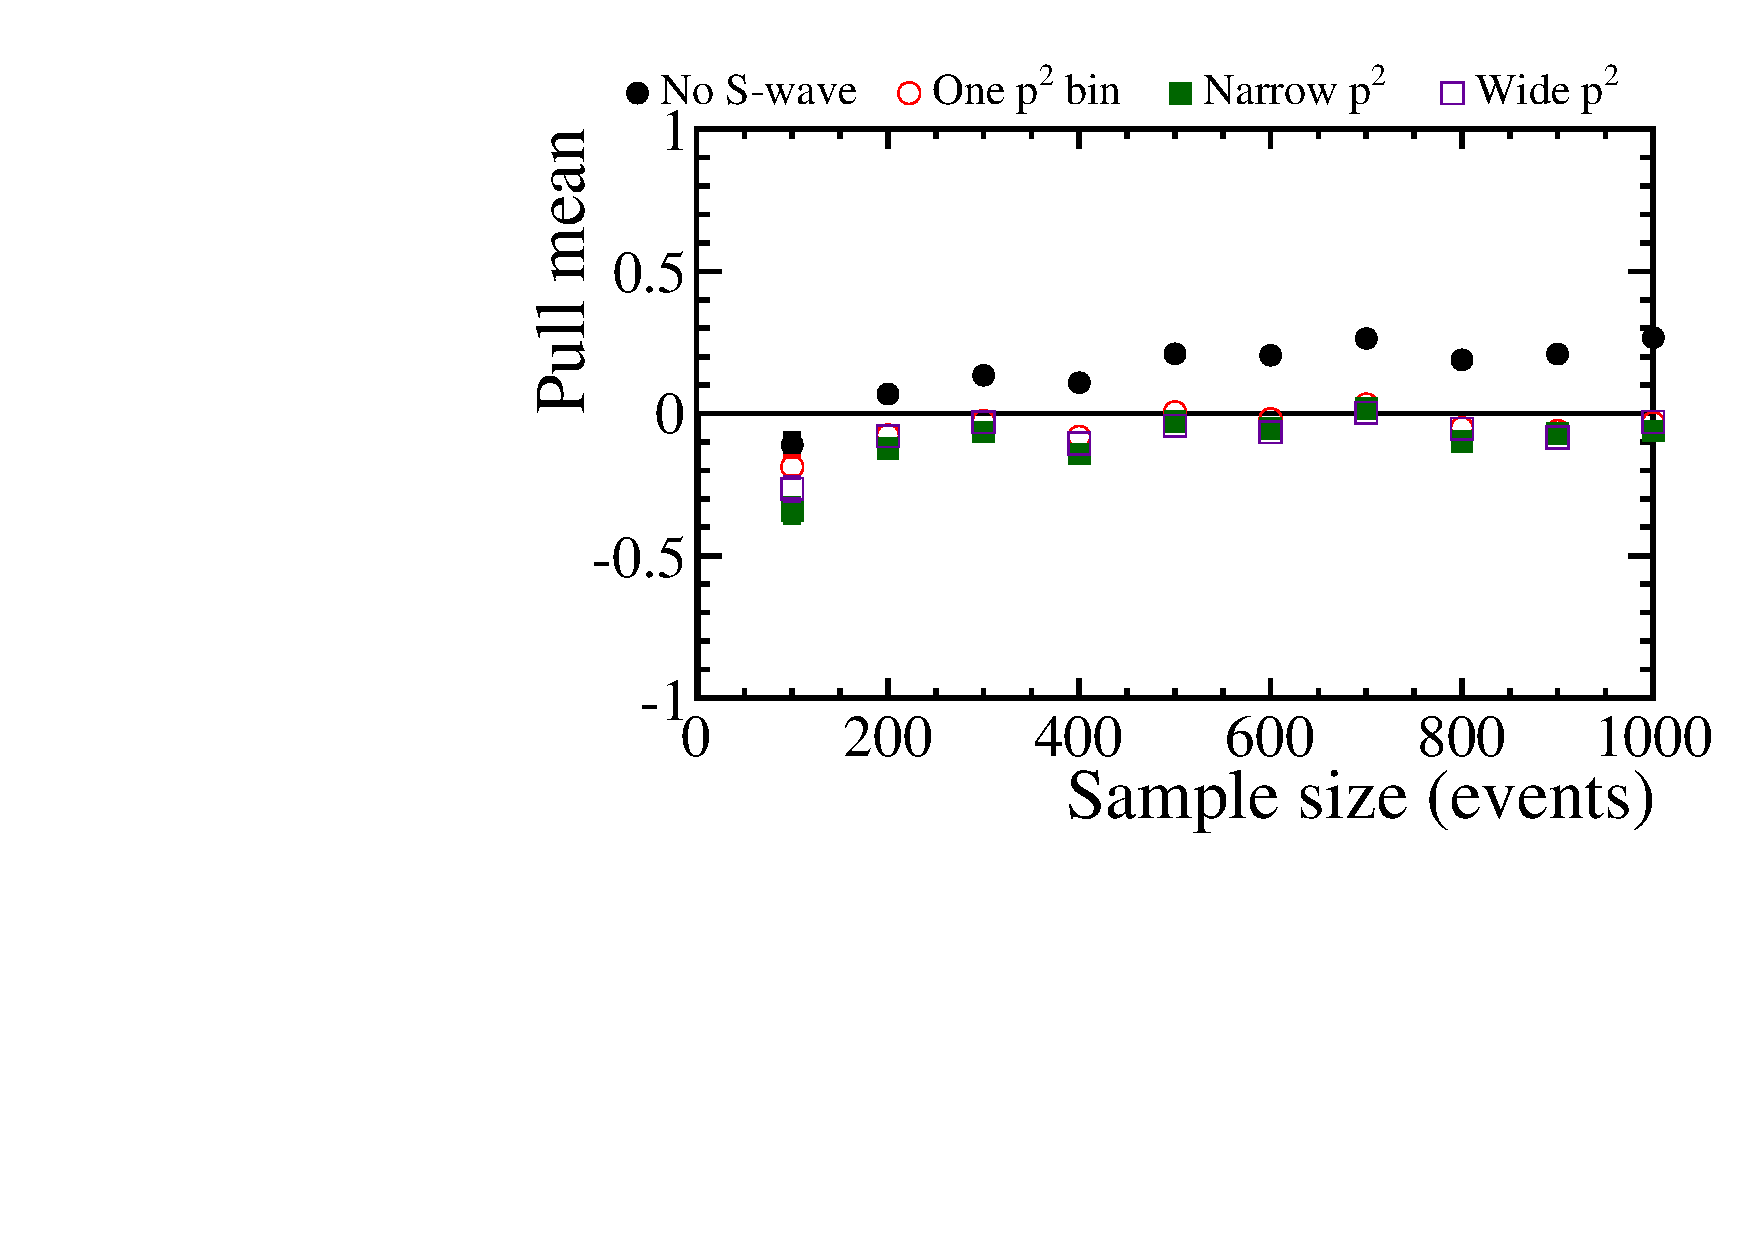
\includegraphics[width=0.48\textwidth]{chapter6/figs/fit_result_combo_ds_afb_mean.pdf}}
\subfigure[\FL]{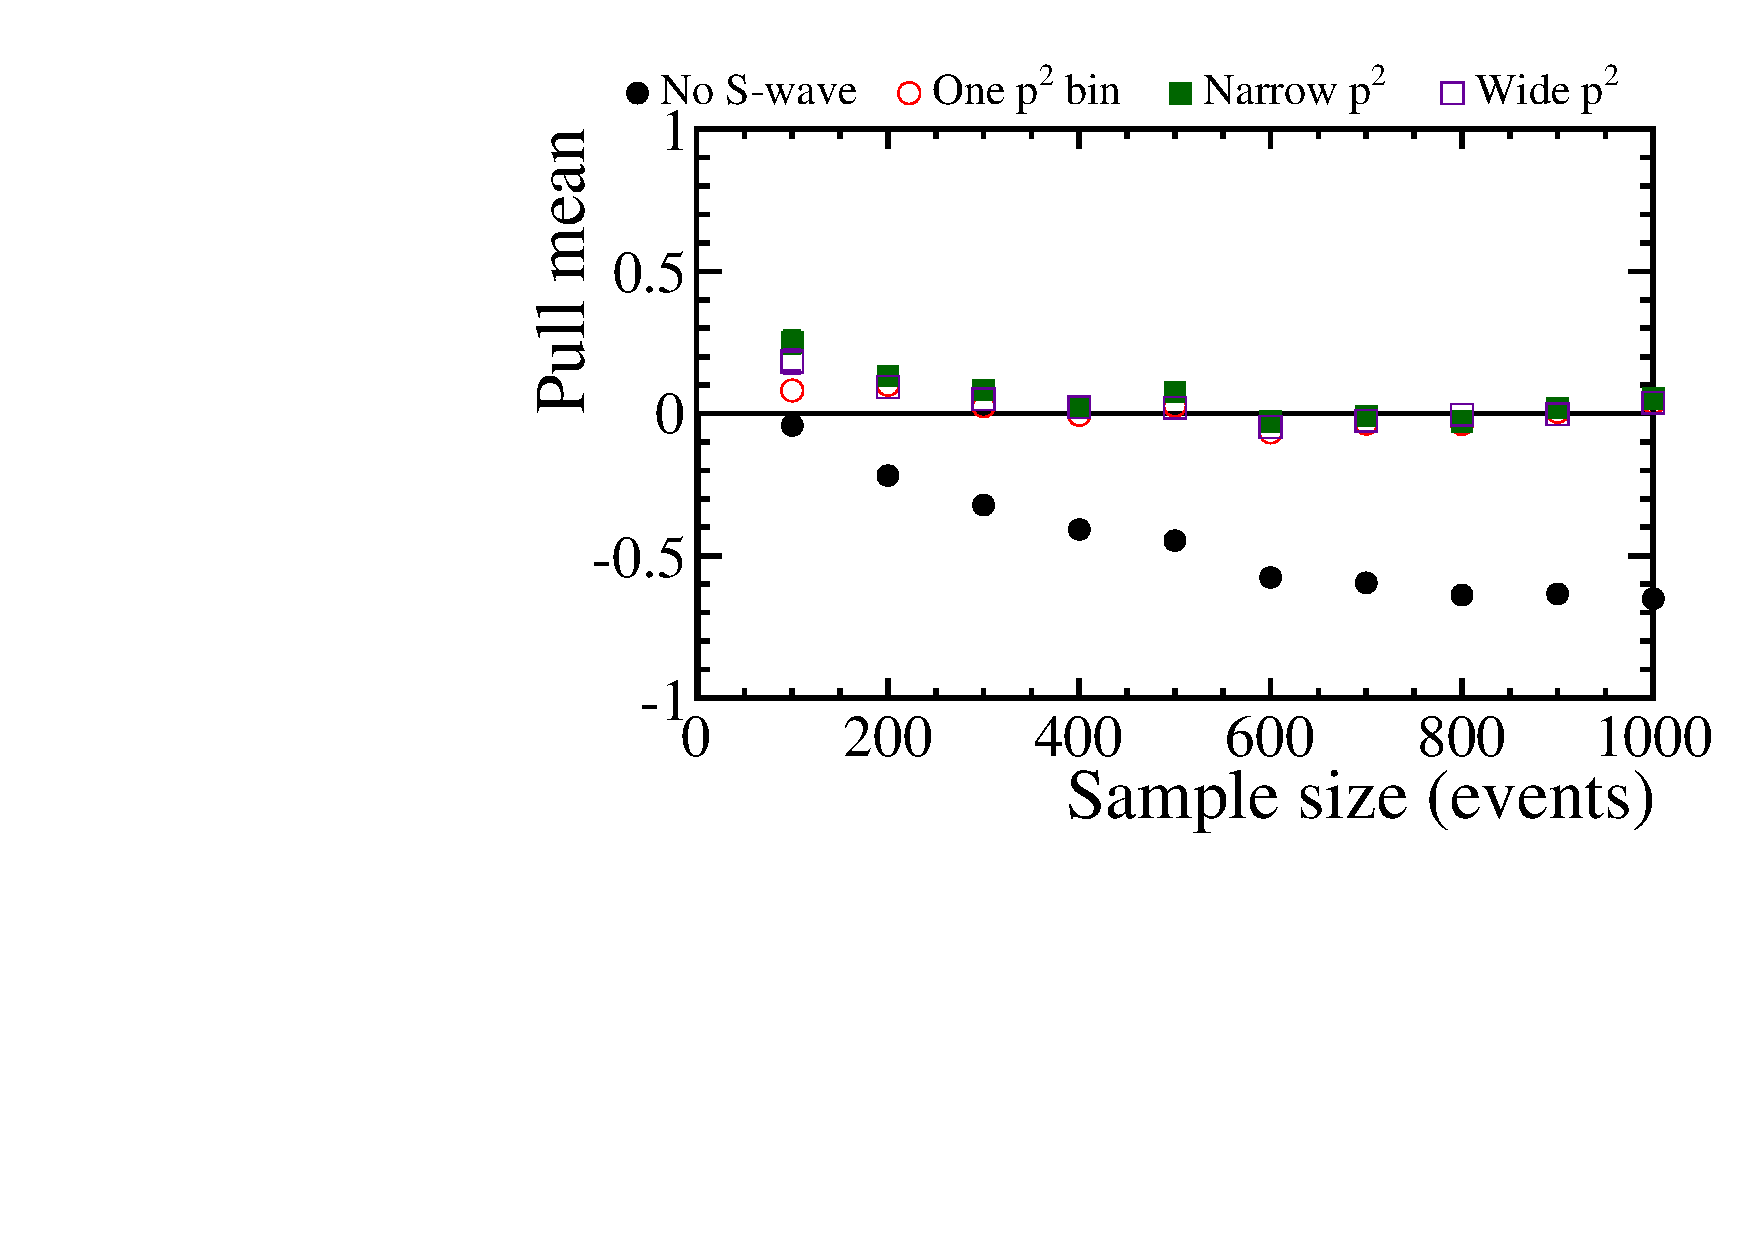
\includegraphics[width=0.48\textwidth]{chapter6/figs/fit_result_combo_ds_fl_mean.pdf}}
\subfigure[\AT2 ]{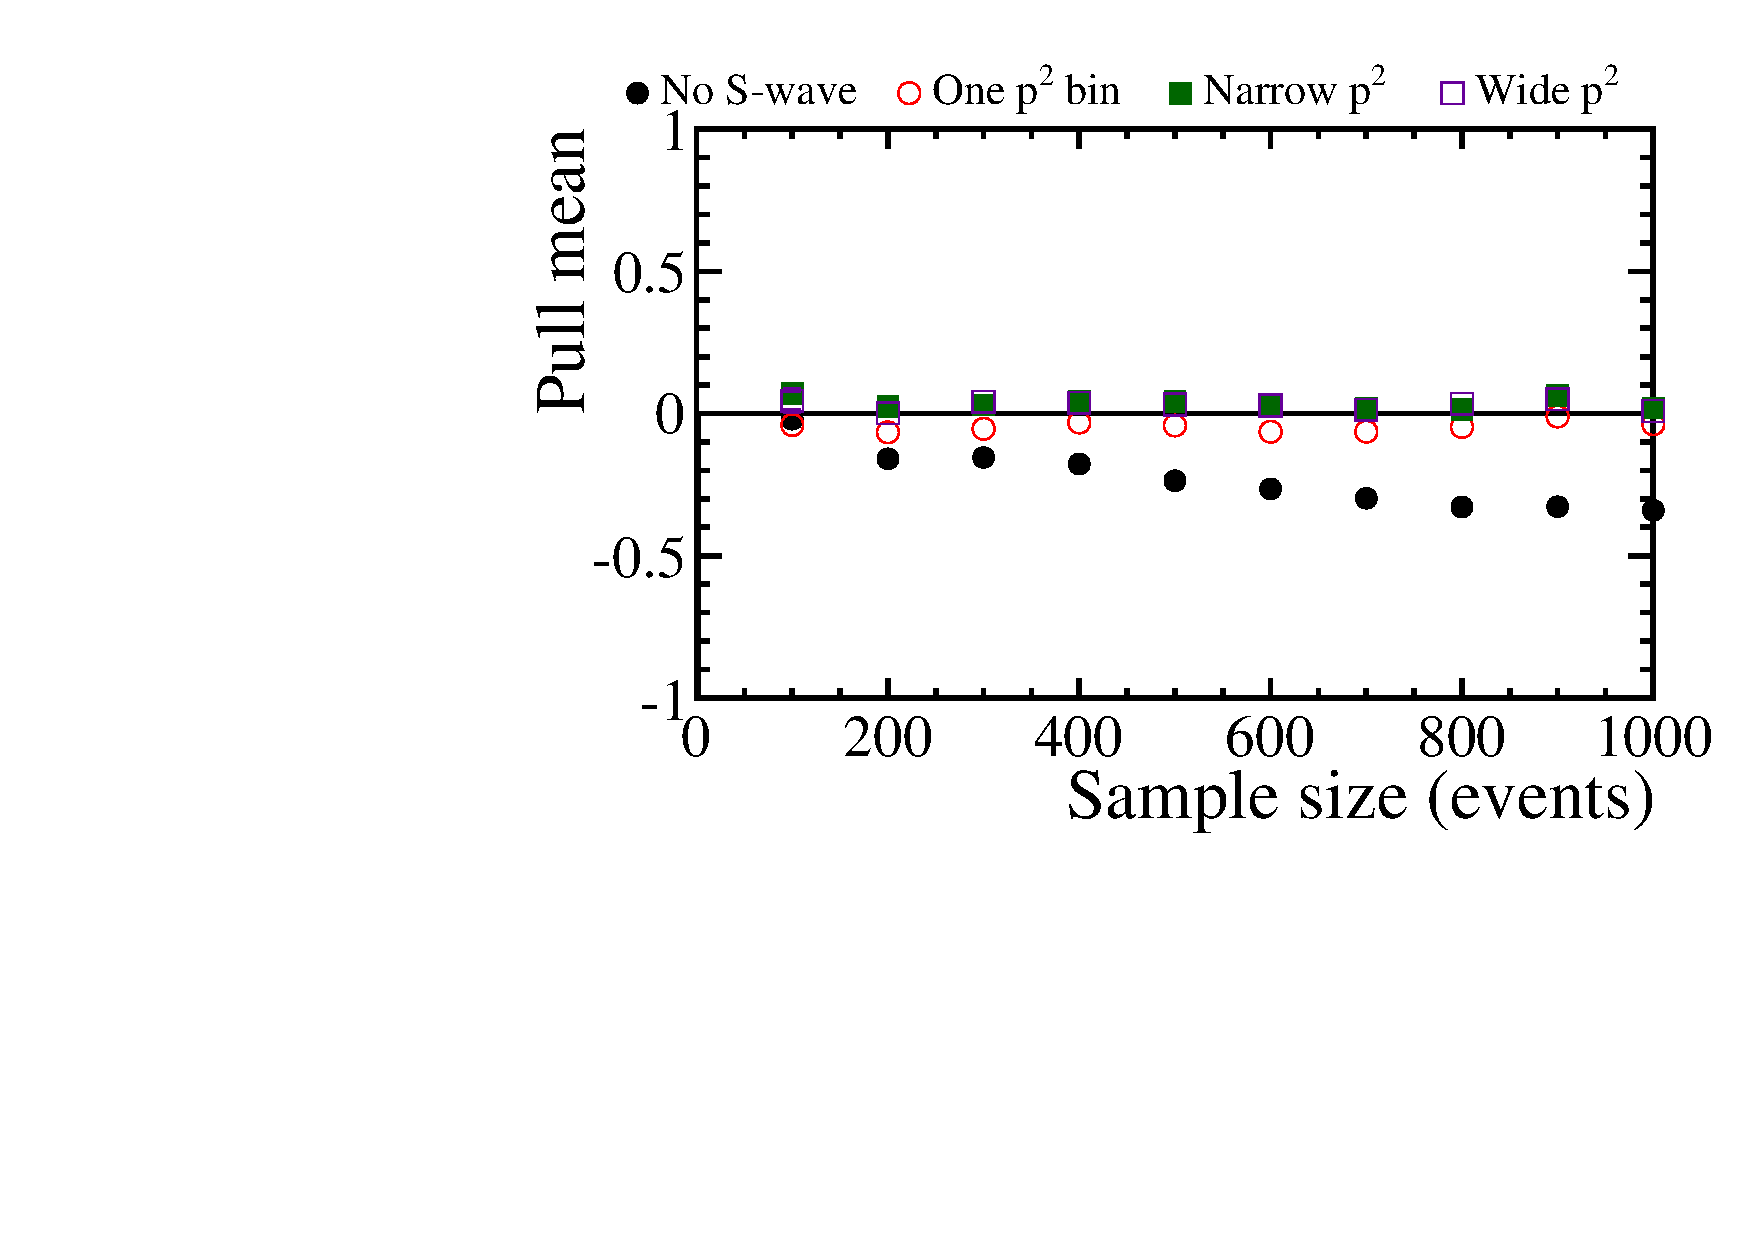
\includegraphics[width=0.48\textwidth]{chapter6/figs/fit_result_combo_ds_at2_mean.pdf}}
\subfigure[\AIm]{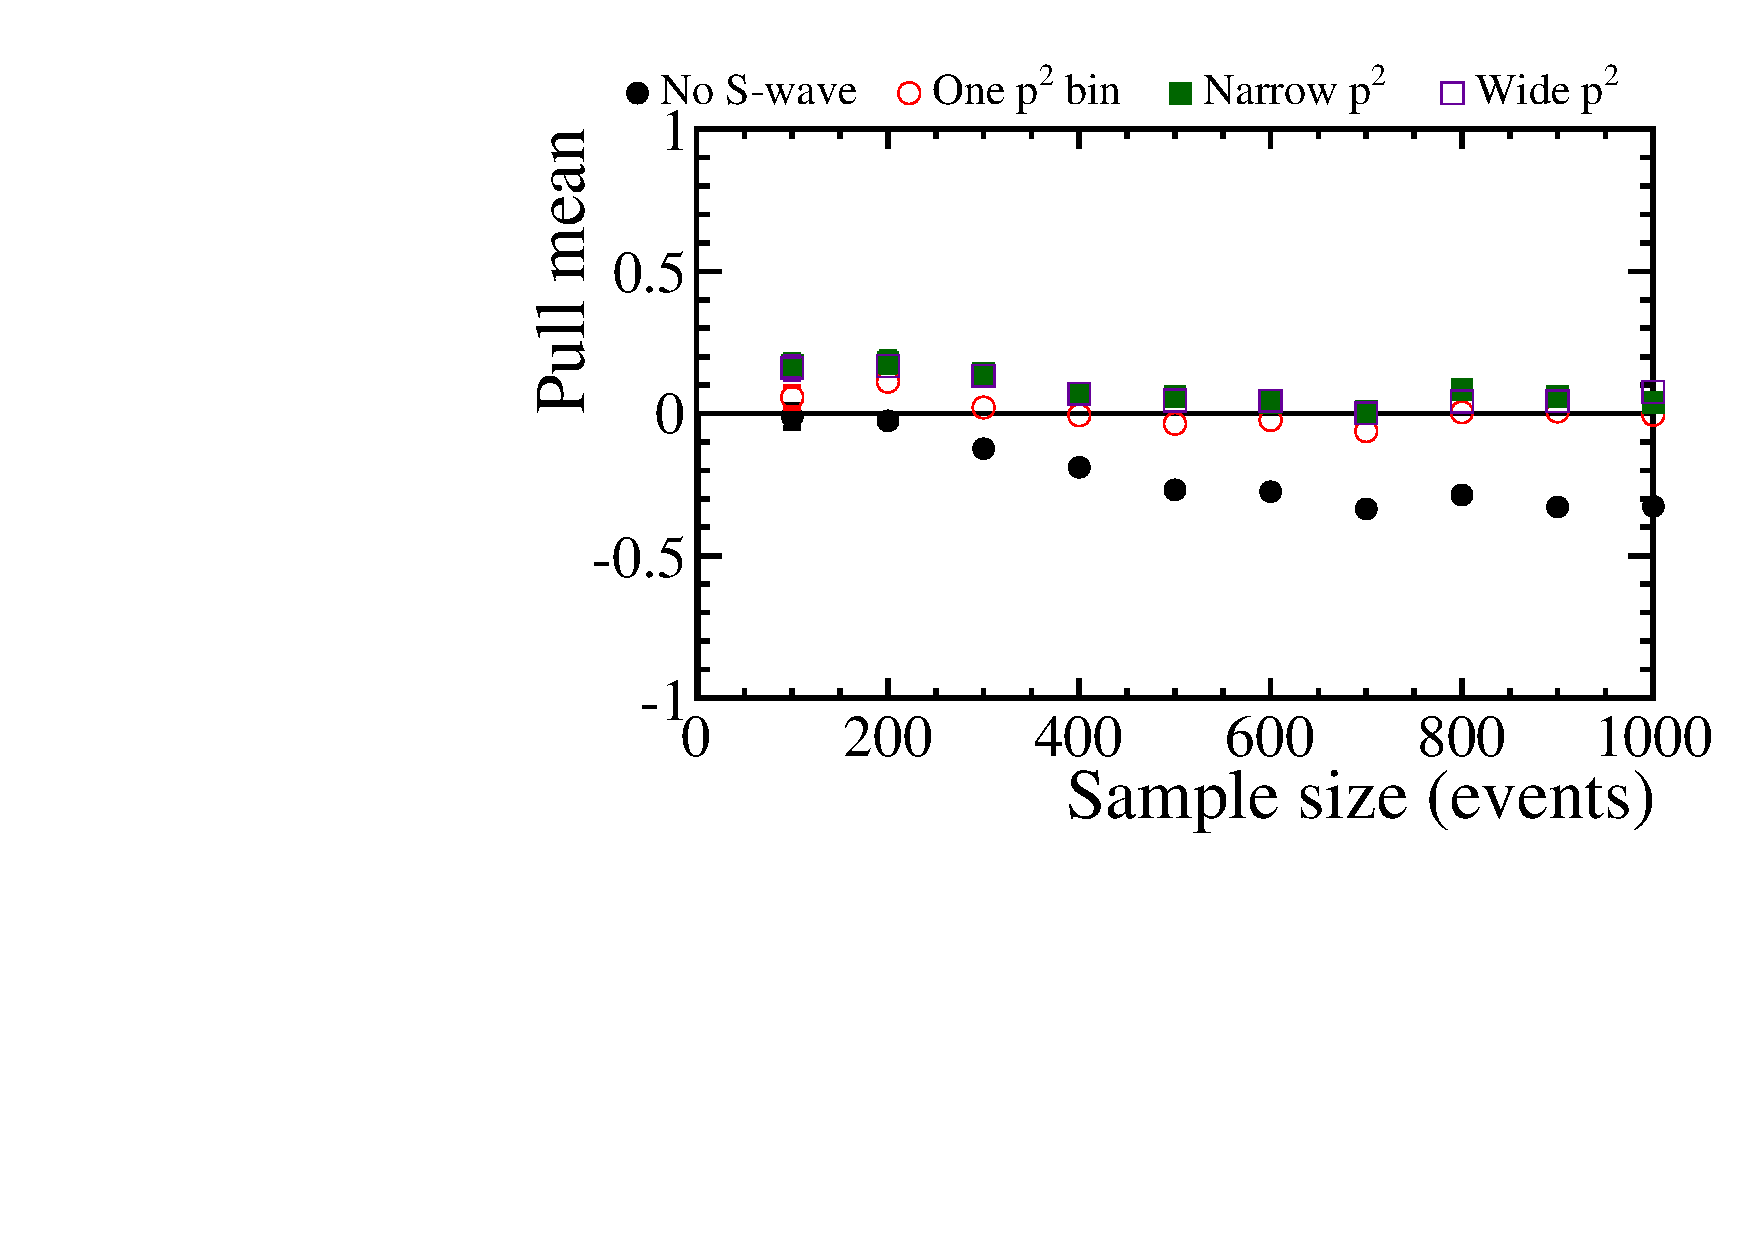
\includegraphics[width=0.48\textwidth]{chapter6/figs/fit_result_combo_ds_aim_mean.pdf}}
\caption[ Pull mean for the three different  
methods to incorporate the S-wave and when the S-wave 
is ignored.      ]
{Pull mean for the three different  
methods to incorporate the S-wave and when the S-wave 
is ignored. There is a slight shift when the S-wave is 
included for datasets of less than 200 events but this is removed from  all the observables 
when the S-wave is included in the fit 
for datasets of over 500 events. ~\label{fig:combods}}
\end{figure}
The pull width for all three fit methods is shown in Fig~\ref{fig:combodswidth}.
\begin{figure}[tb]
\centering
\subfigure[\AFB]{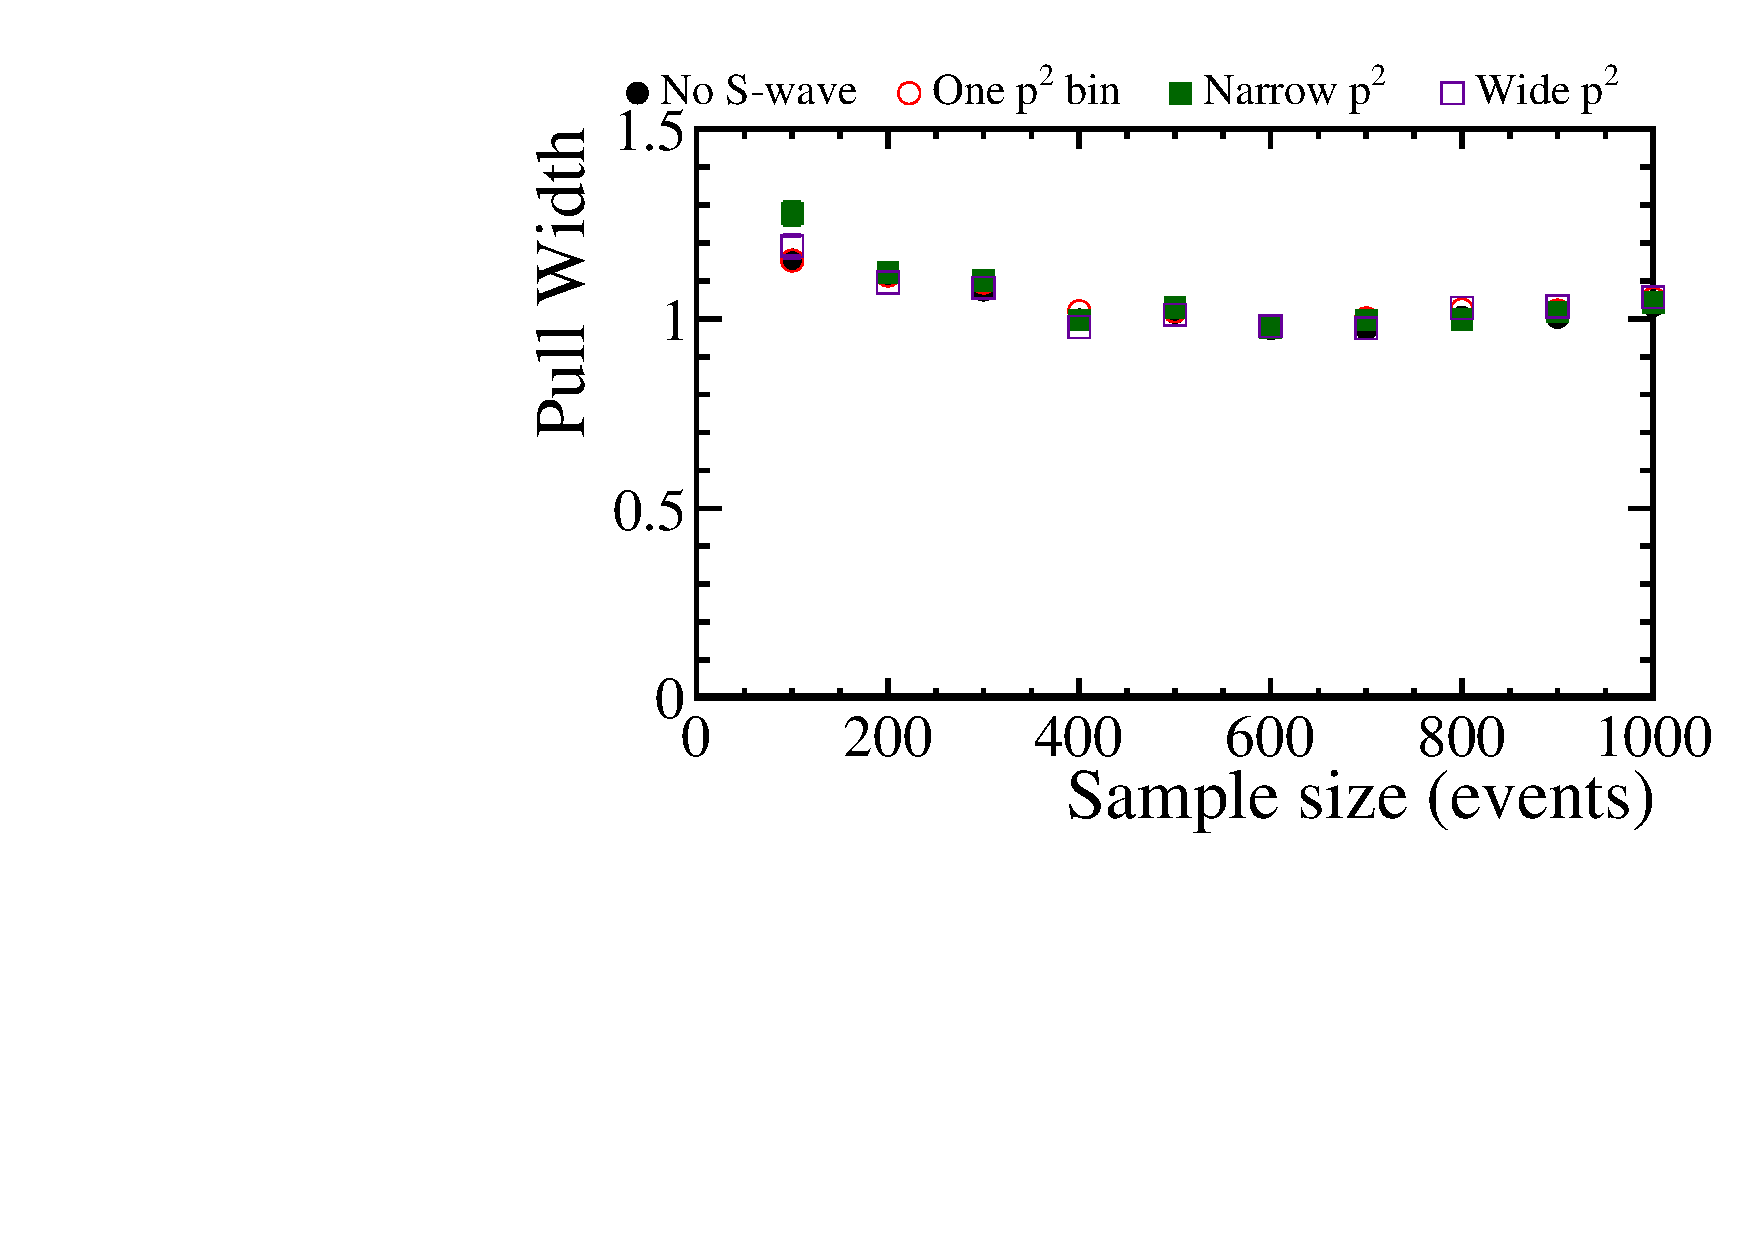
\includegraphics[width=0.48\textwidth]{chapter6/figs/fit_result_combo_ds_afb_width.pdf}}
\subfigure[\FL]{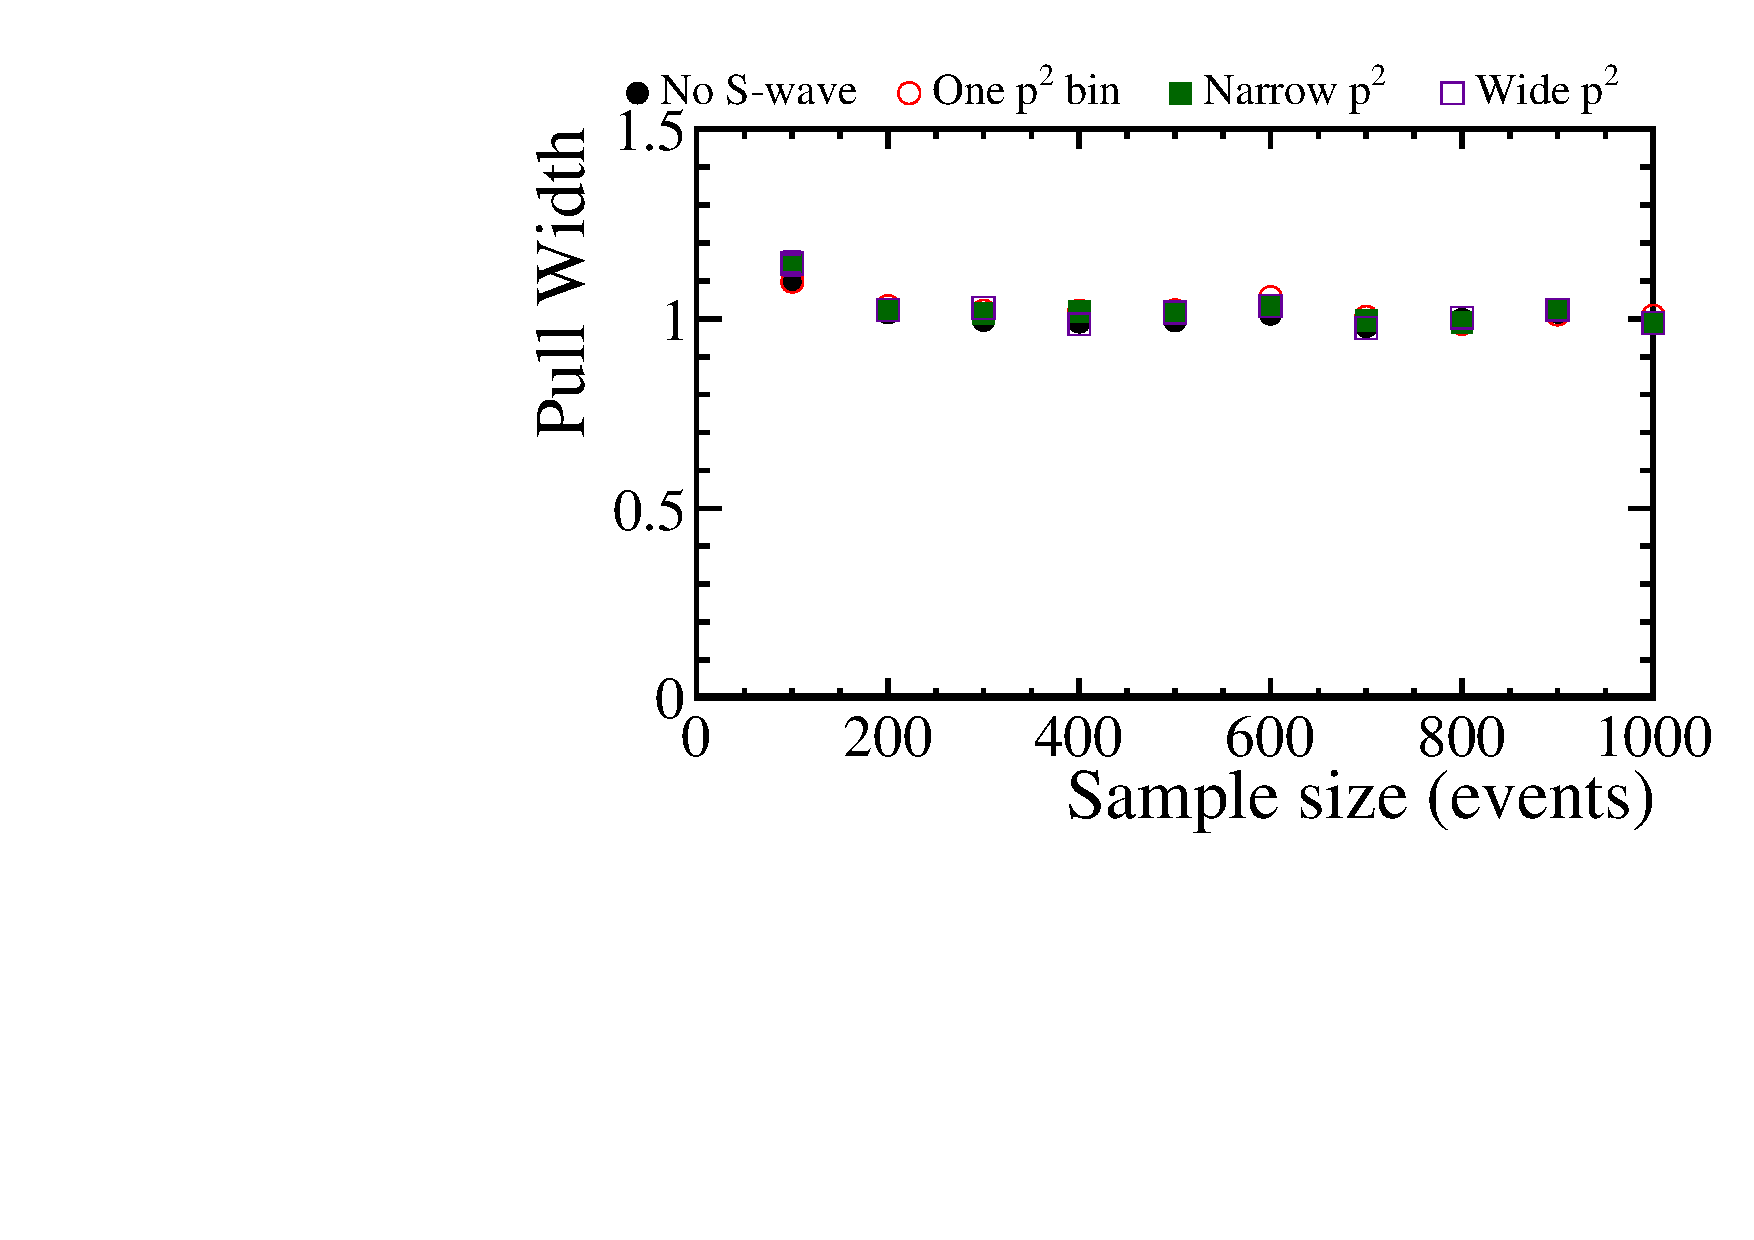
\includegraphics[width=0.48\textwidth]{chapter6/figs/fit_result_combo_ds_fl_width.pdf}}
\subfigure[\AT2 ]{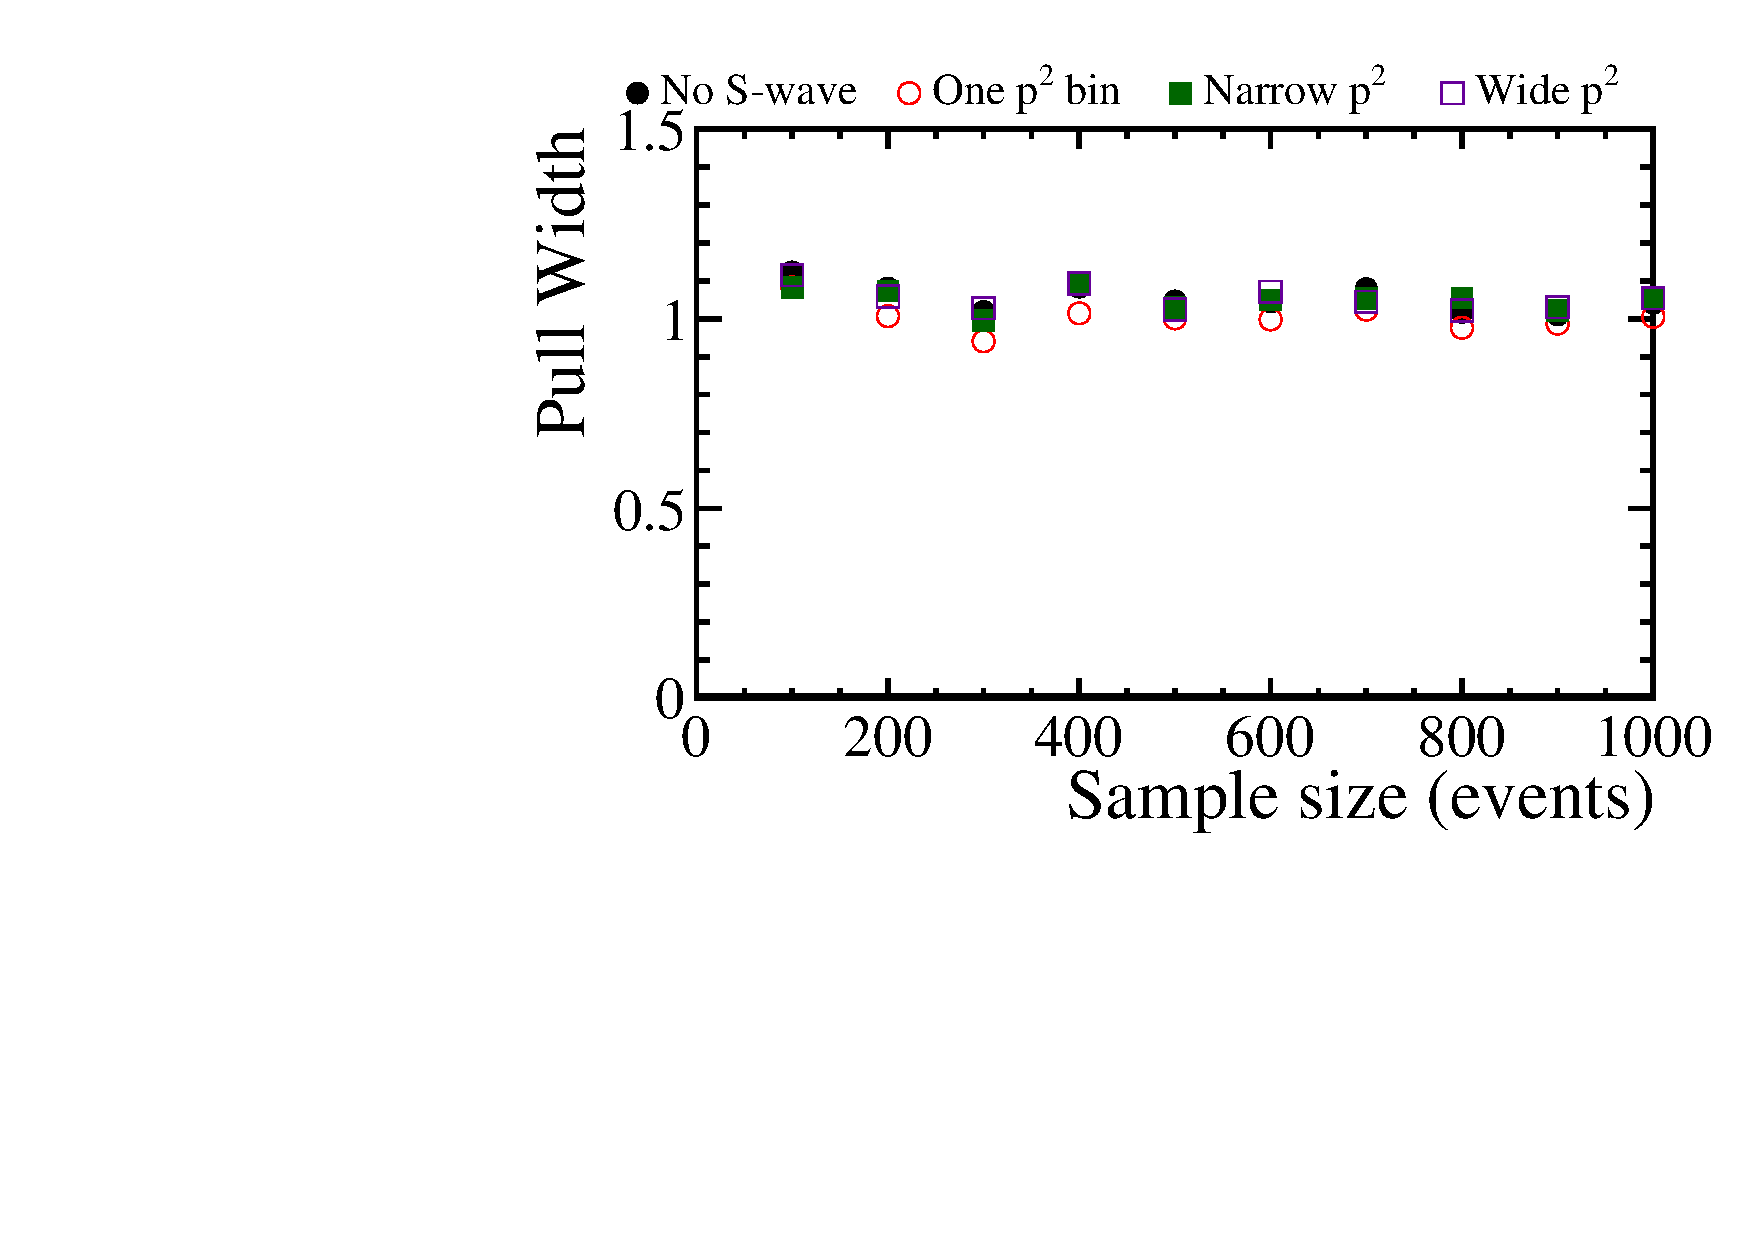
\includegraphics[width=0.48\textwidth]{chapter6/figs/fit_result_combo_ds_at2_width.pdf}}
\subfigure[\AIm]{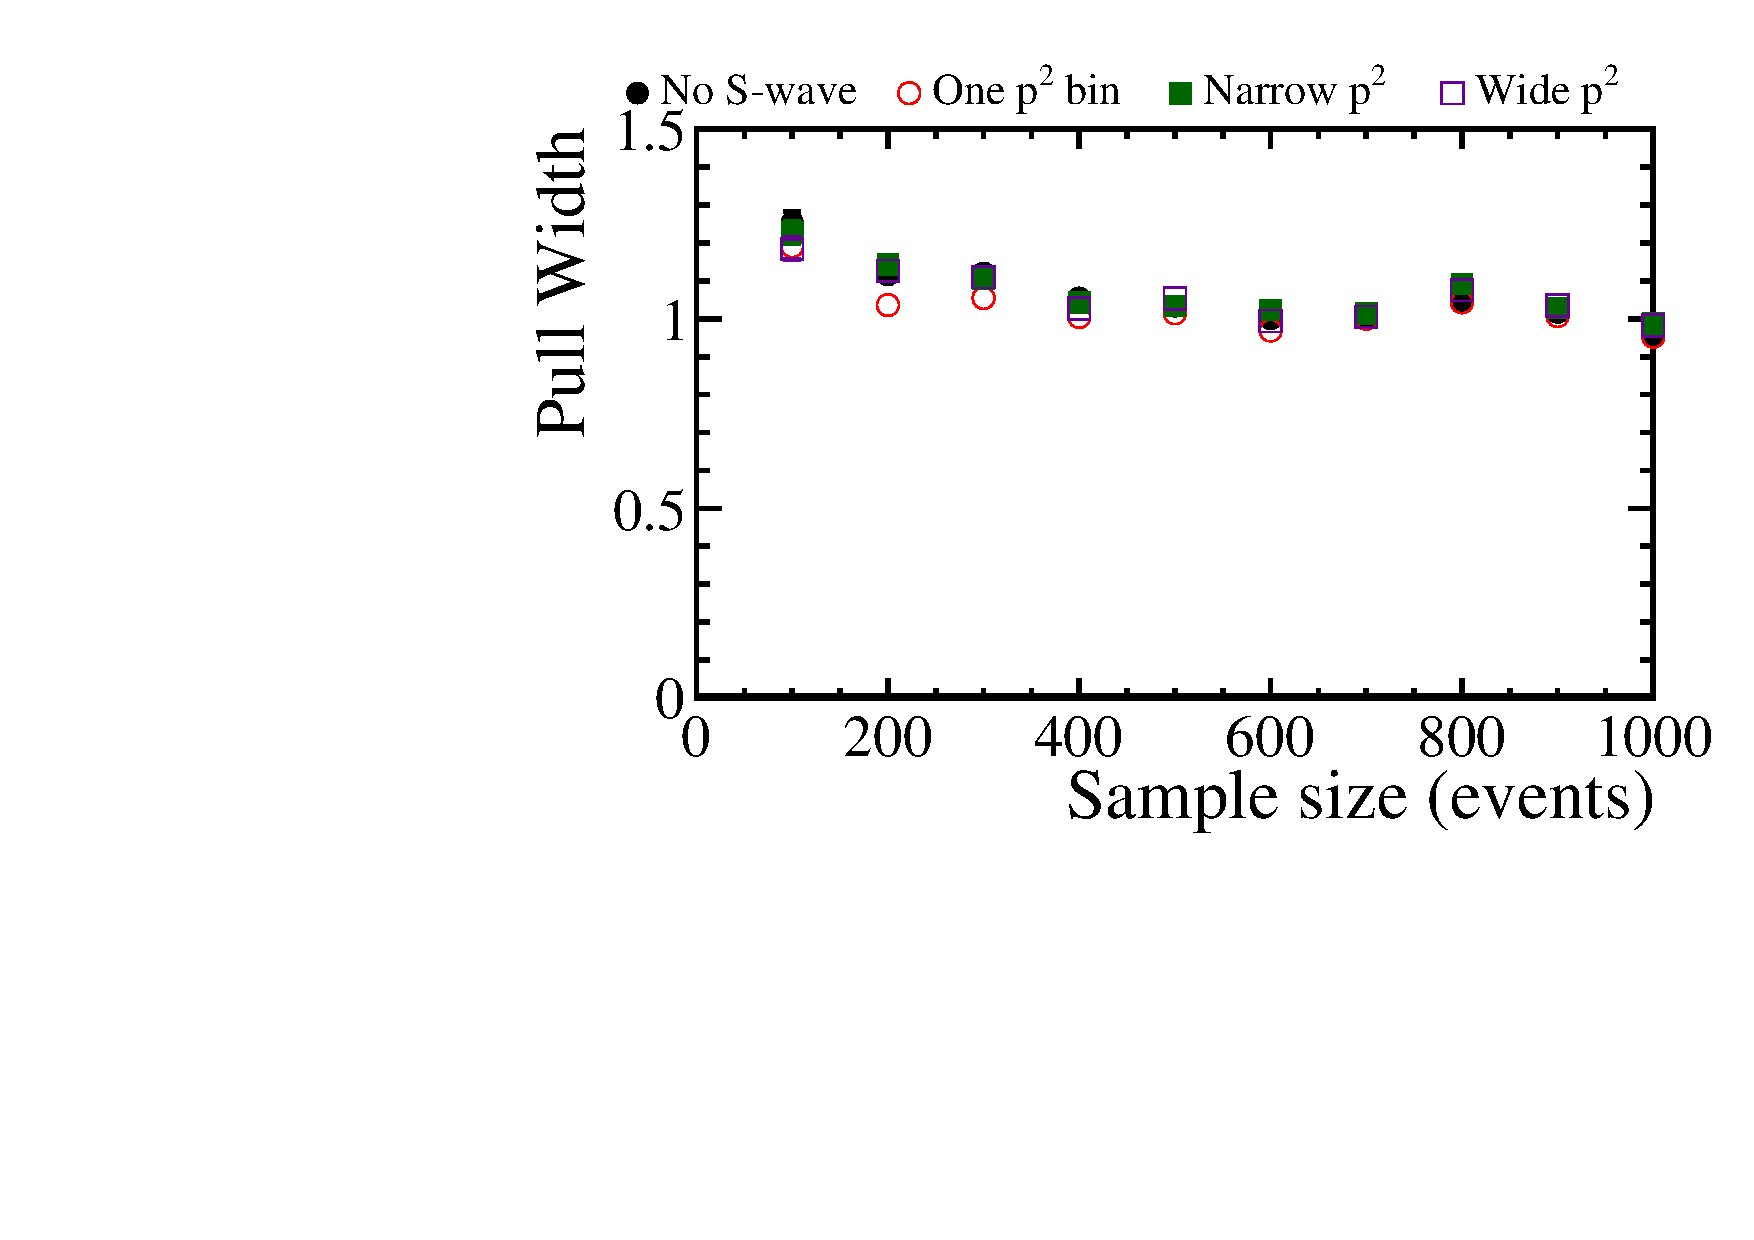
\includegraphics[width=0.48\textwidth]{chapter6/figs/fit_result_combo_ds_aim_width.pdf}}
\caption[ Pull width for the three different  
methods to incorporate the S-wave and when the S-wave 
is ignored.  ]
{Pull width for the three different  
methods to incorporate the S-wave and when the S-wave 
is ignored. There is a slight shift when the S-wave is 
included for datasets of less than 200 events but this is removed from  all the observables 
when the S-wave is included in the fit 
for datasets of over 500 events. ~\label{fig:combodswidth}}
\end{figure}

For all observables, it can be seen that the resolution degrades when
the S-wave is included and the \psq dependence is ignored.  The
resolution degrades by a smaller amount when the \psq dependence is
included in a small bin and the original resolution is recovered to
within 10\% when using the large \psq range.  There are two effects
contributing to the improvement of the resolution. There are more
P-wave events in the larger range and the wider mass window allows for
the S-wave to be constrained by using the information from above and
below the P-wave resonance.  This results in the best resolution when
the S-wave is included in the angular distribution.

For all the observables, the pull mean approaches zero for datasets of
greater than 300 events implying that the bias present in the
observables when a pure P-wave state is assumed is removed when an S-wave is
included in the angular distribution. This means that the inclusion of
the S-wave component will be mandatory for all future experimental
analyses.


The ratio of the resolutions for the three different fit methods
as a function of increasing S-wave size is given in Fig.~\ref{fig:ratiofs}.
\begin{figure}[tb]
\centering
\subfigure[\AFB]{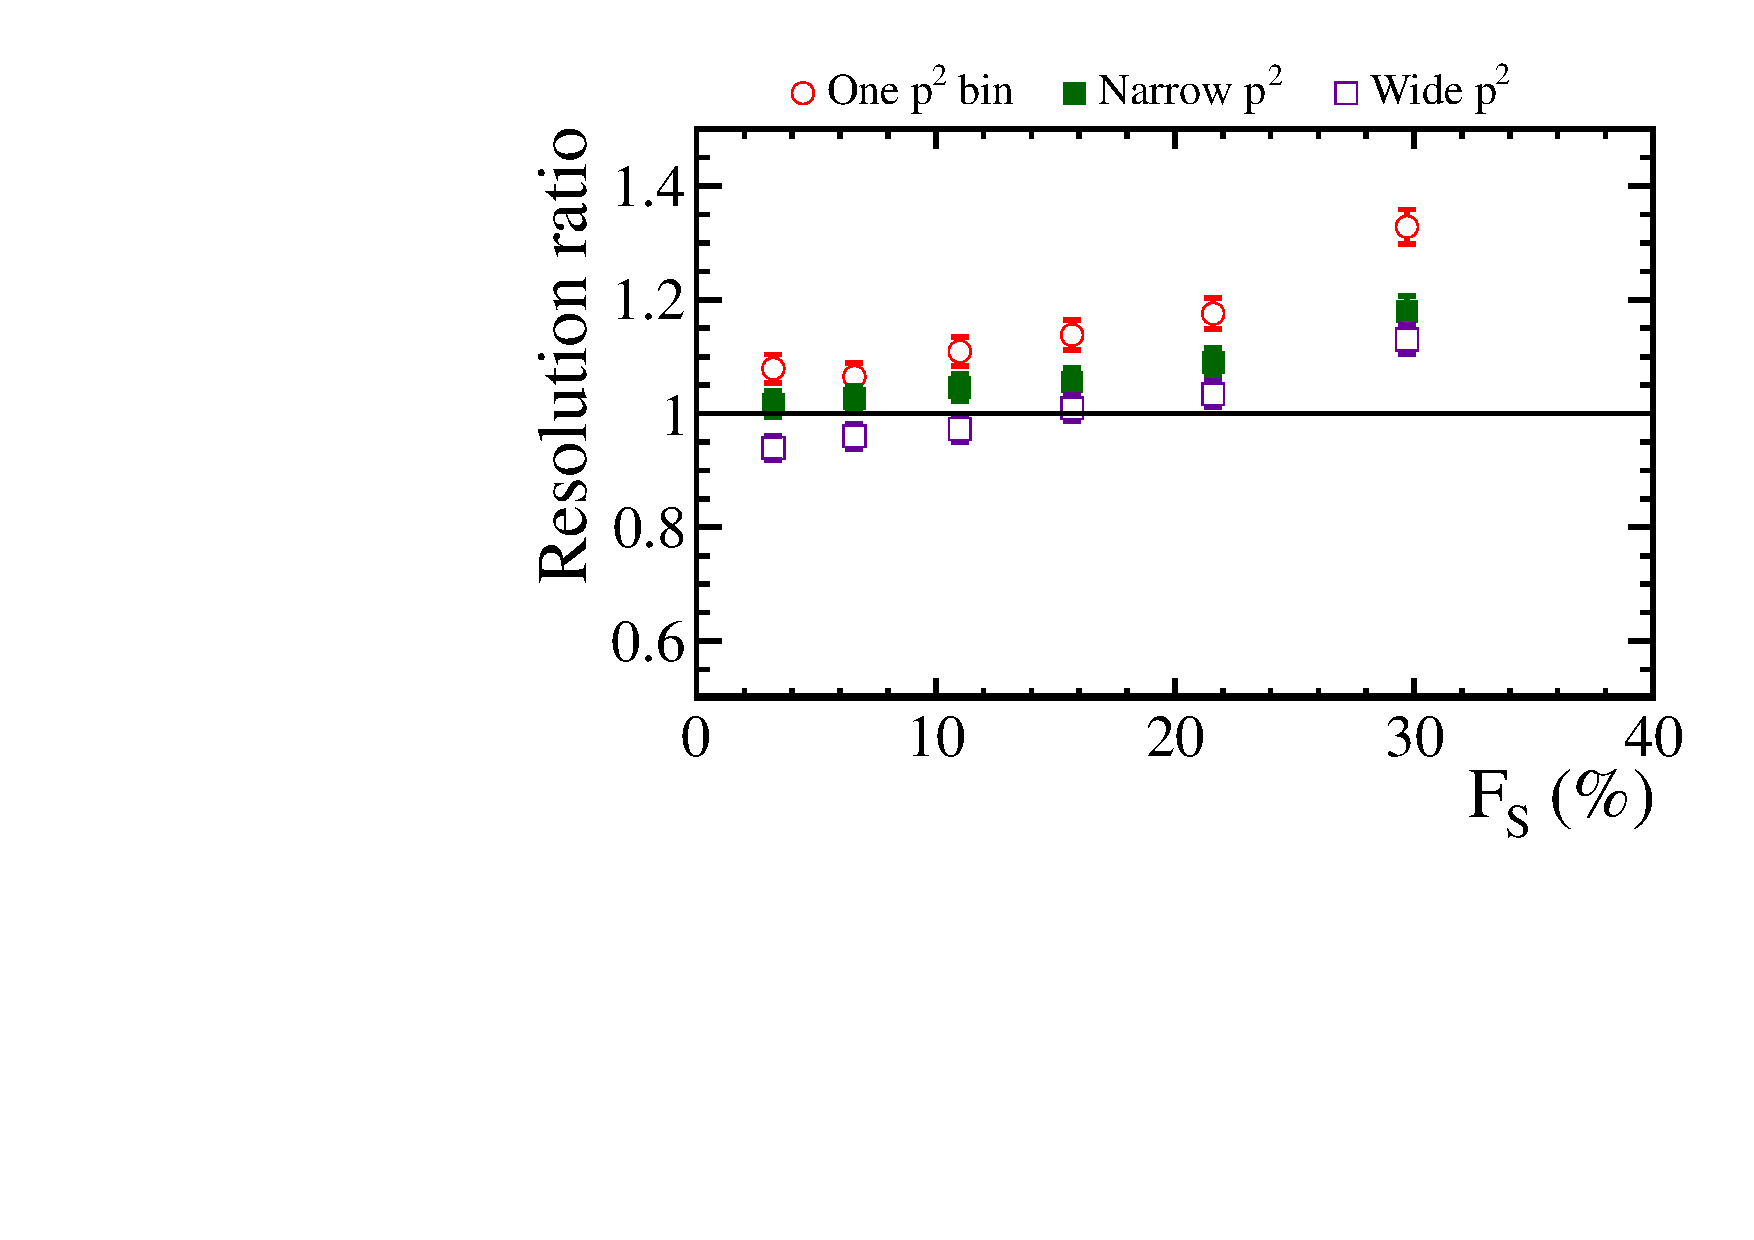
\includegraphics[width=0.48\textwidth]{chapter6/figs/fit_result_ratio_fs_afb_res.pdf}}
\subfigure[\FL]{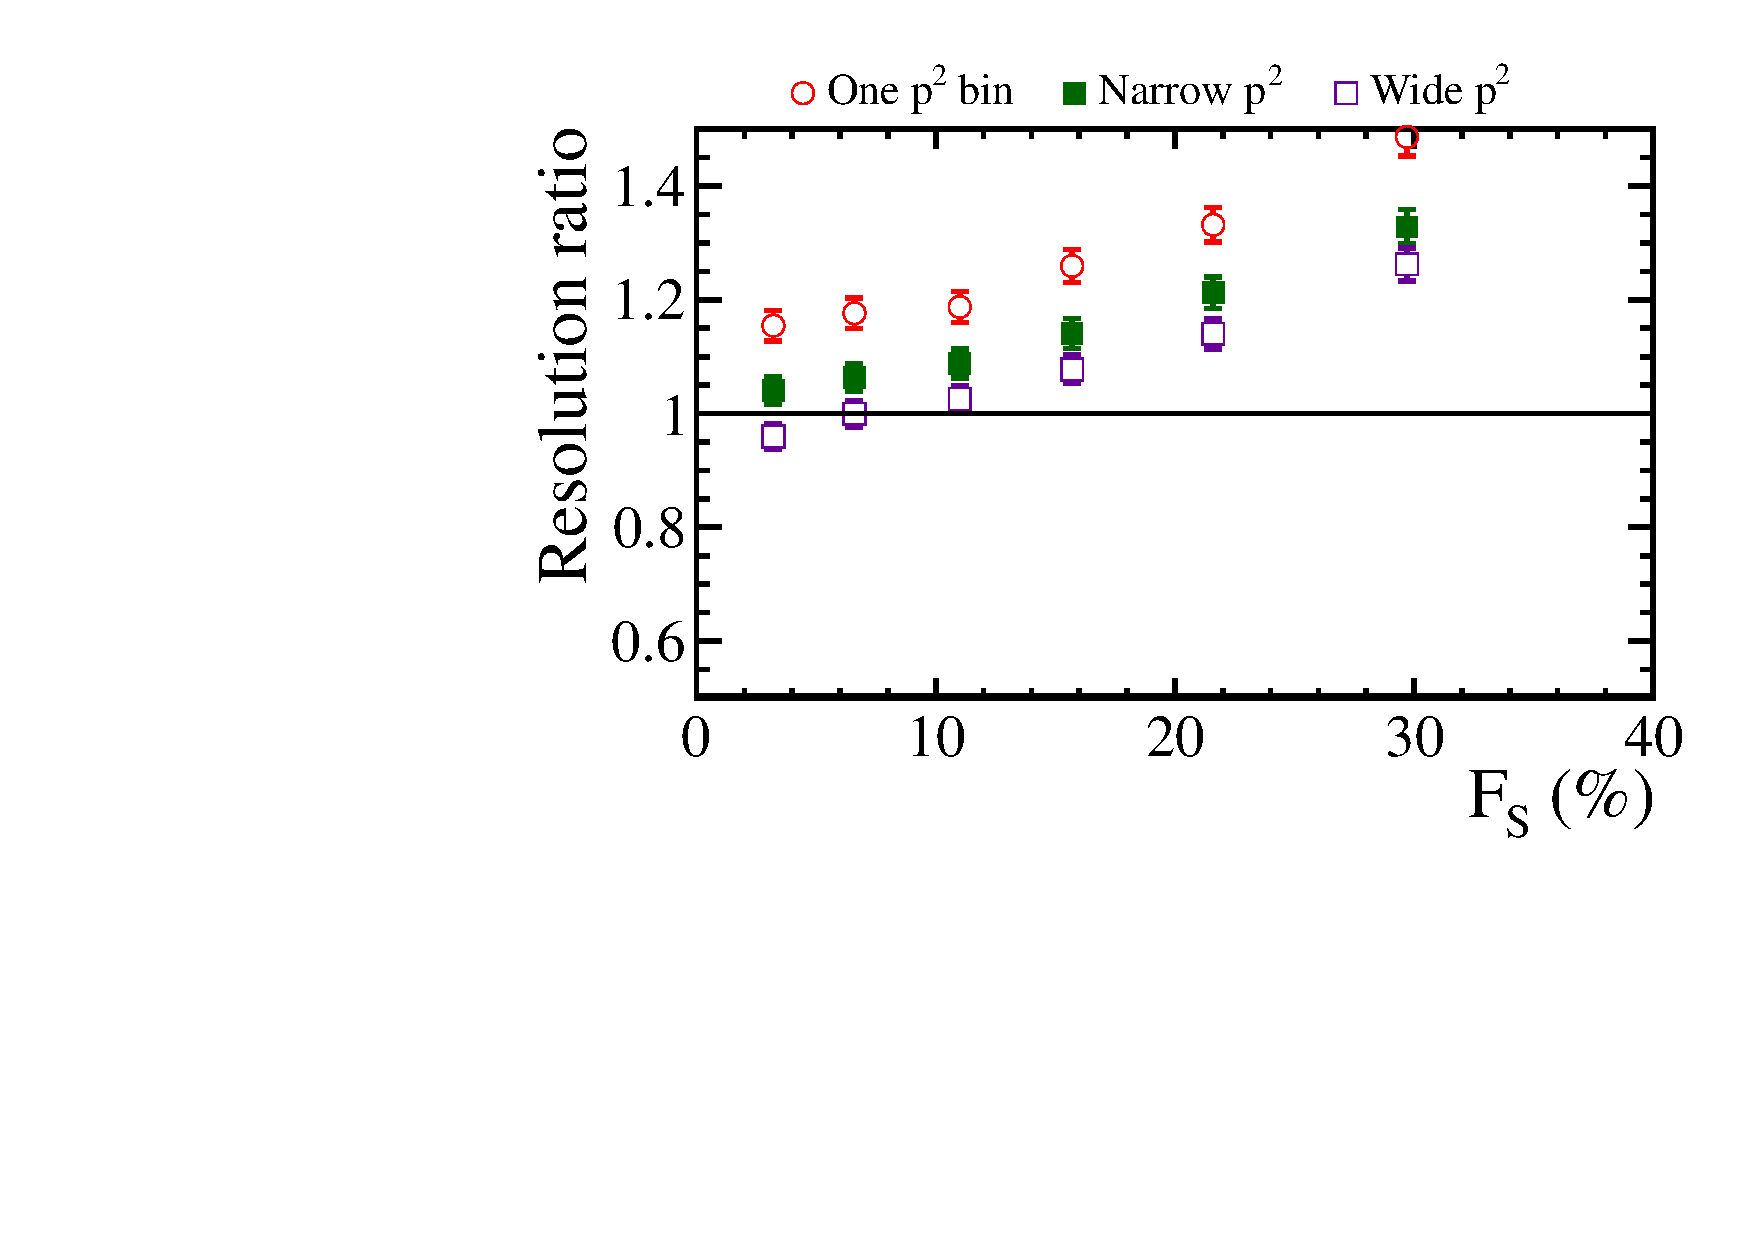
\includegraphics[width=0.48\textwidth]{chapter6/figs/fit_result_ratio_fs_fl_res.pdf}}
\subfigure[\AT2 ]{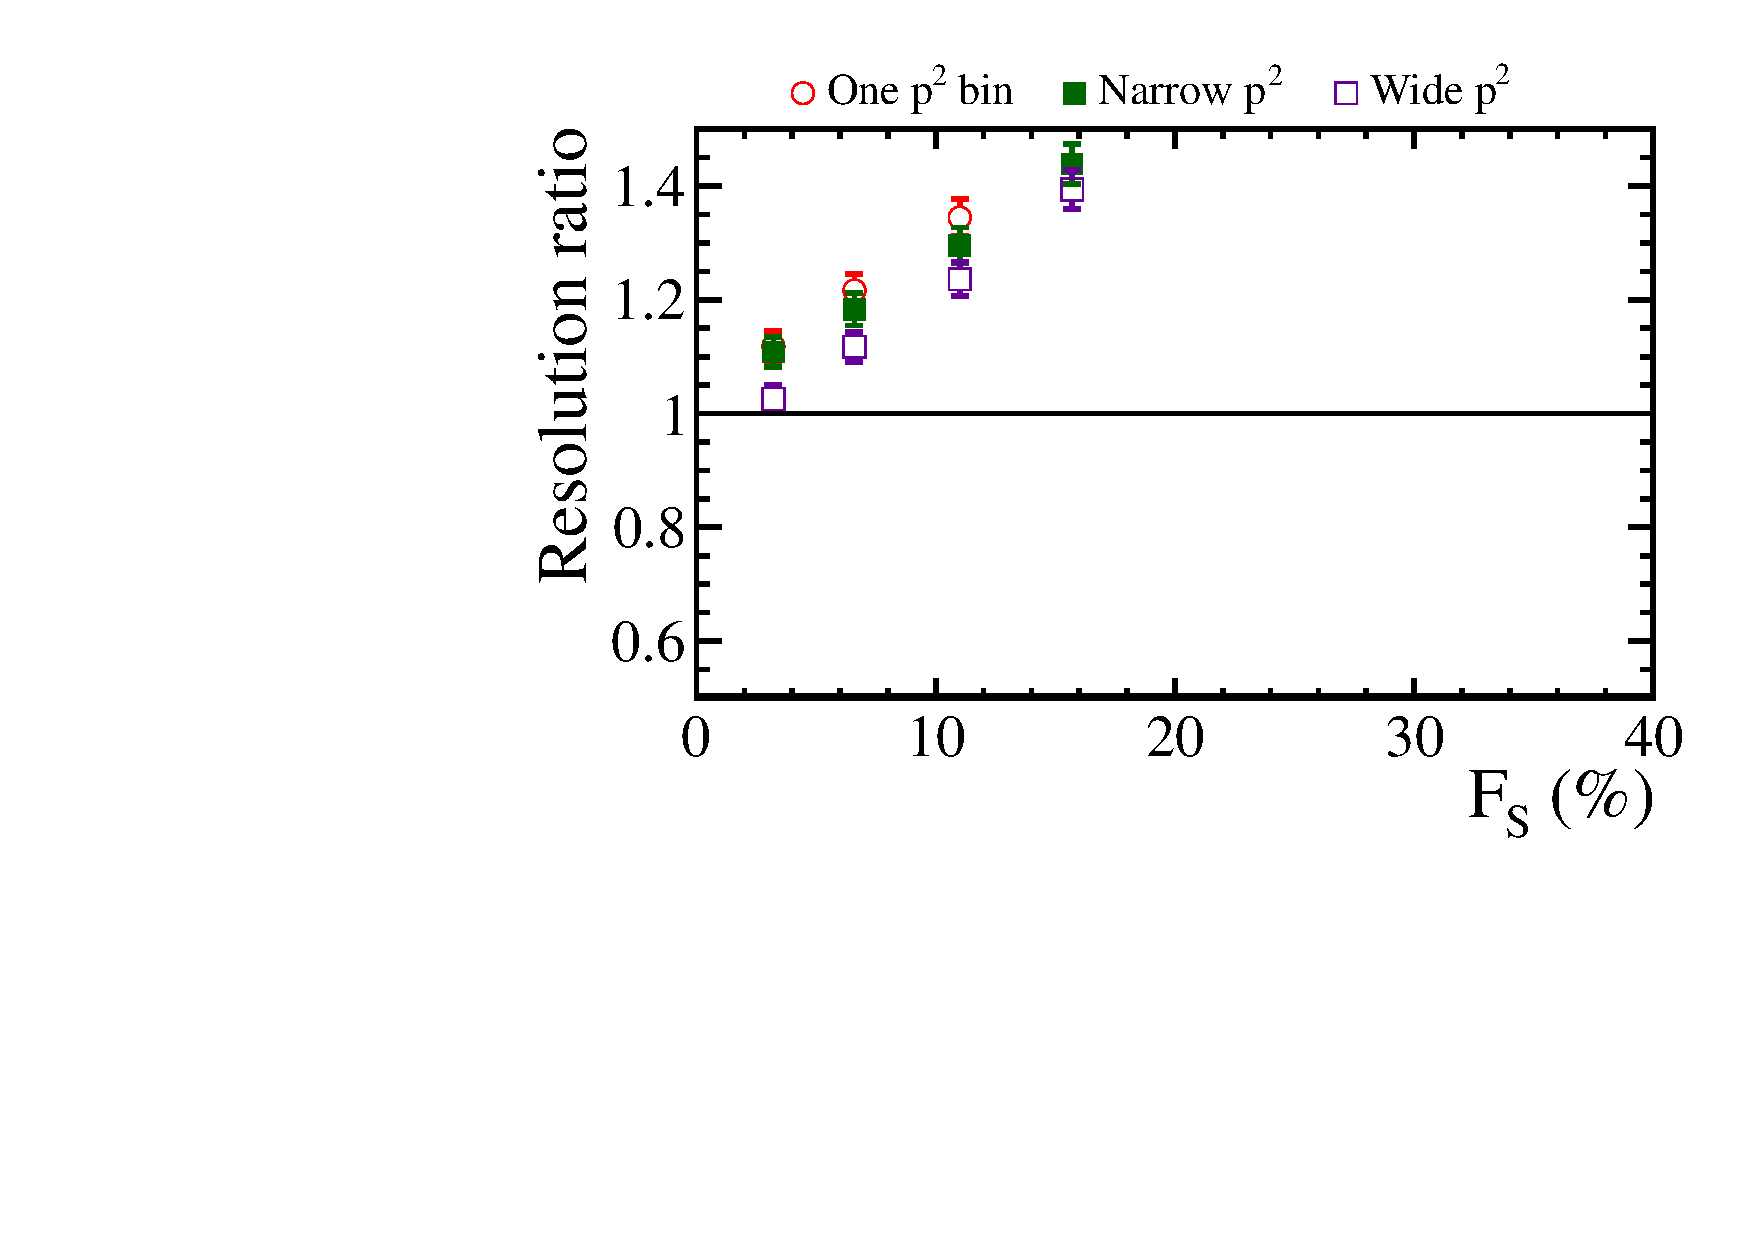
\includegraphics[width=0.48\textwidth]{chapter6/figs/fit_result_ratio_fs_at2_res.pdf}}
\subfigure[\AIm]{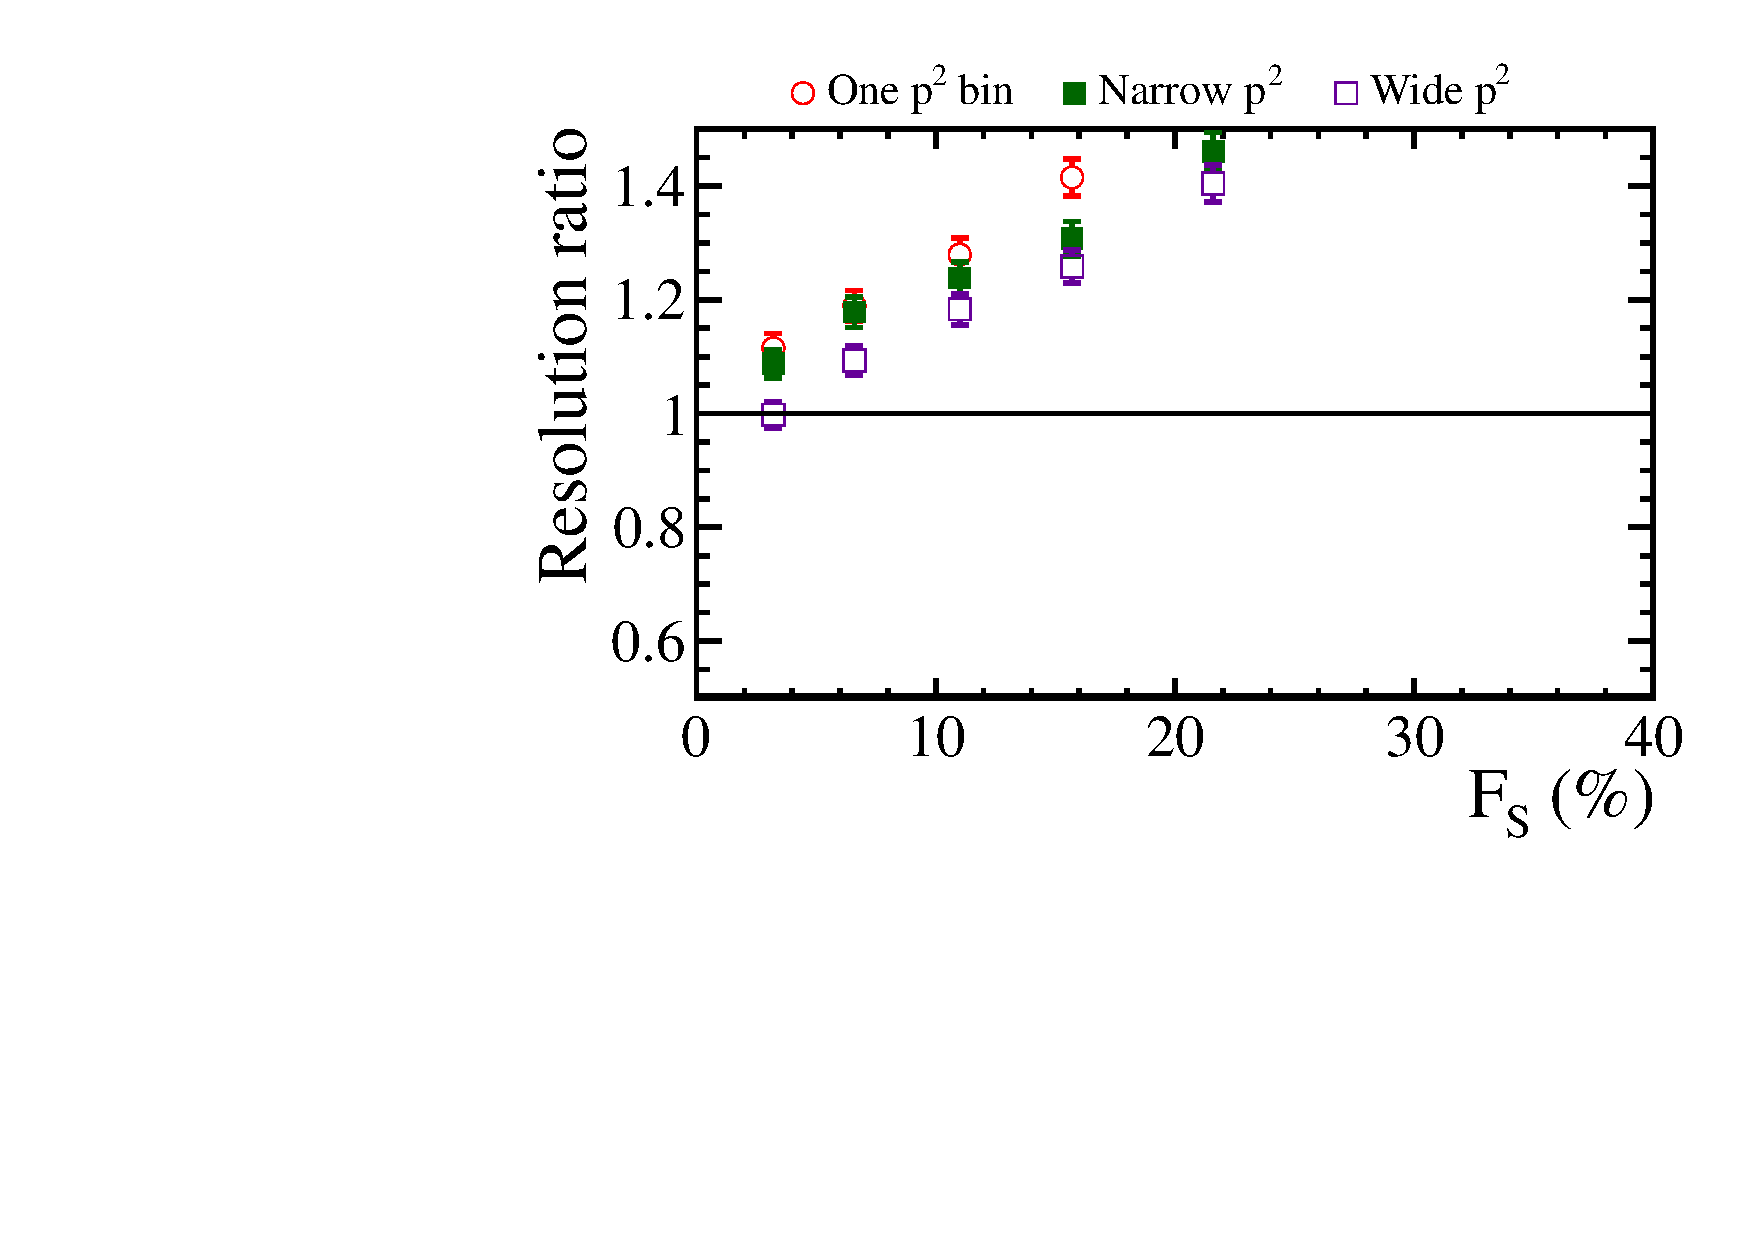
\includegraphics[width=0.48\textwidth]{chapter6/figs/fit_result_ratio_fs_aim_res.pdf}}
\caption[  Resolutions for three different methods to incorporate 
the S-wave relative to the resolution obtained when the S-wave is ignored.   ]
{Resolutions for three different methods to incorporate 
the S-wave relative to the resolution obtained when the S-wave is ignored. 
It can be seen that the best resolution is obtained when using the largest \psq window.
The original resolution is recovered to within 10\%. ~\label{fig:ratiofs}}
\end{figure}
The pull mean  as a function of S-wave contribution 
for all three fit methods is shown in Fig.~\ref{fig:combofs}.
\begin{figure}[tb]
\centering
\subfigure[\AFB]{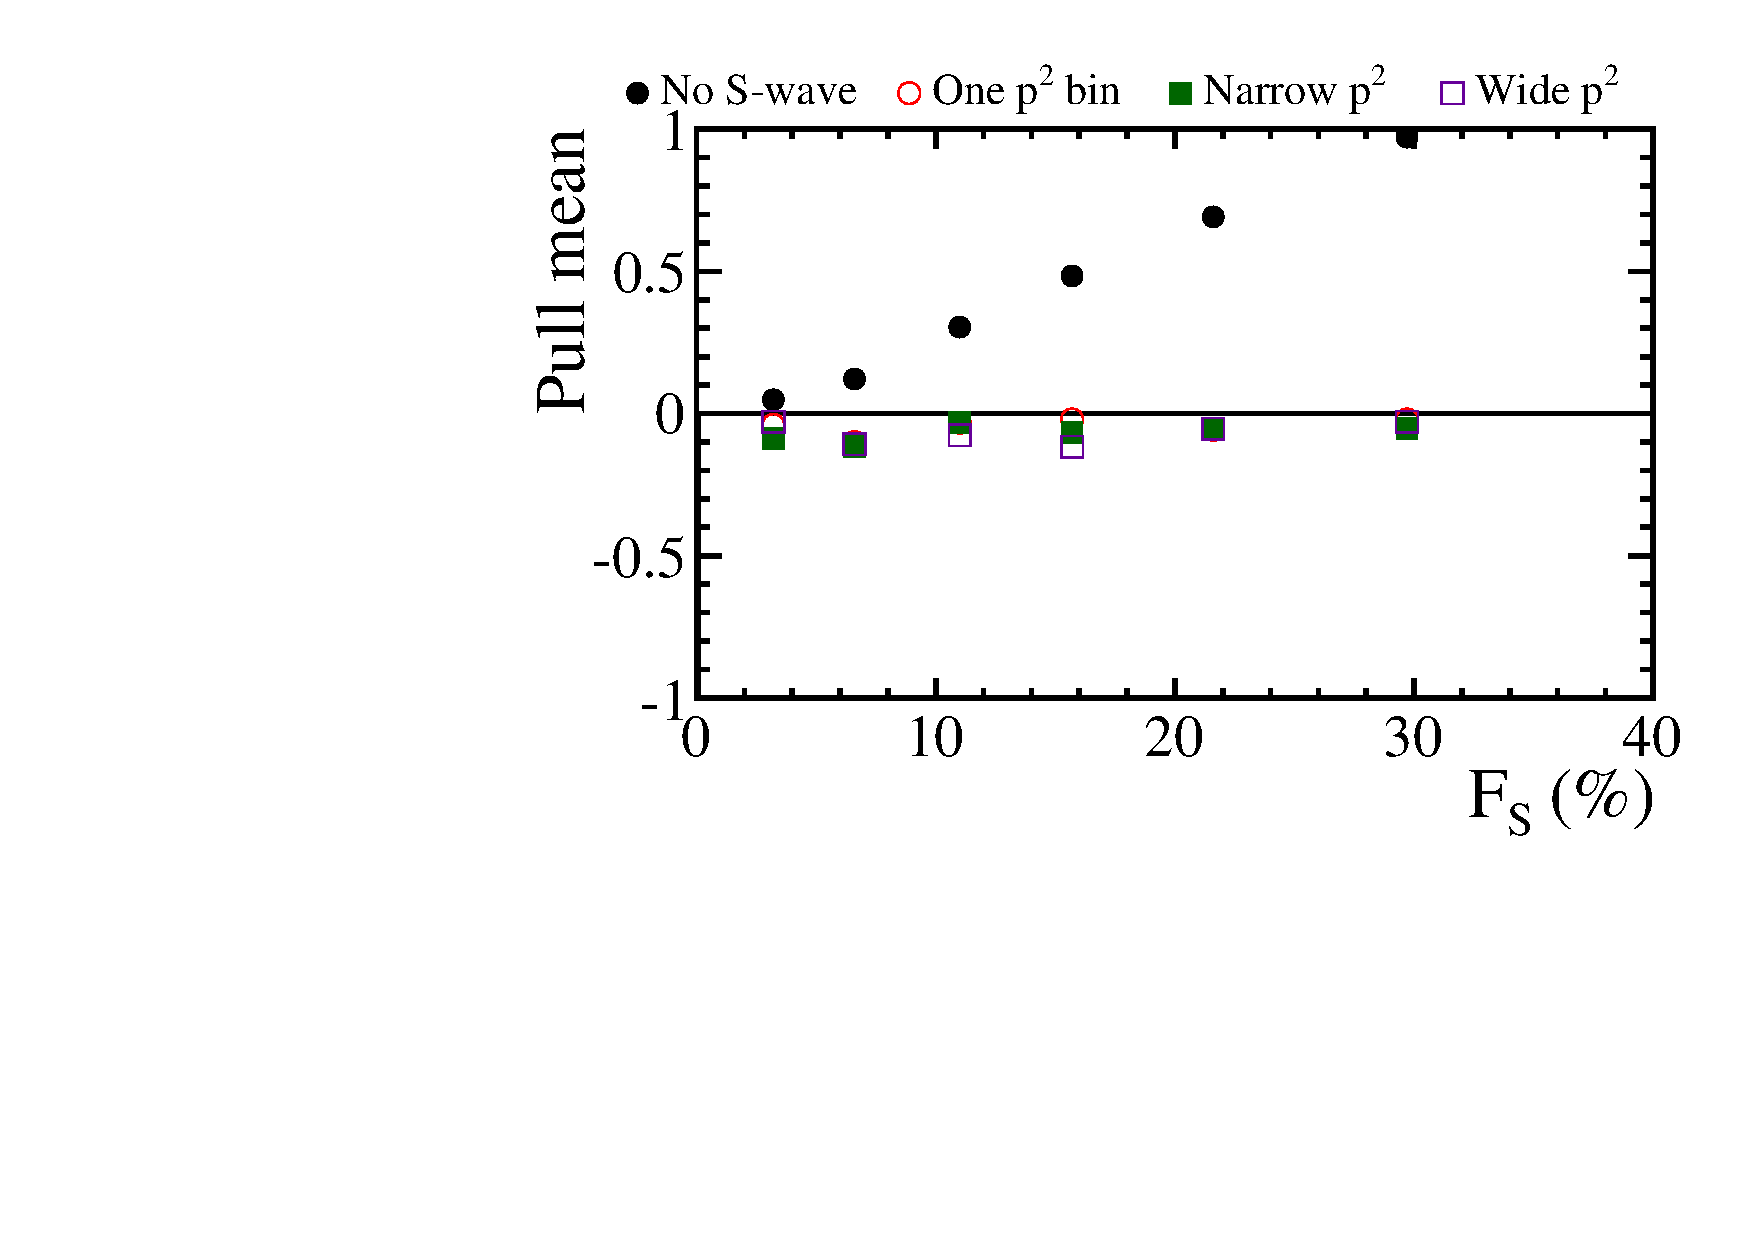
\includegraphics[width=0.48\textwidth]{chapter6/figs/fit_result_combo_fs_afb_mean.pdf}}
\subfigure[\FL]{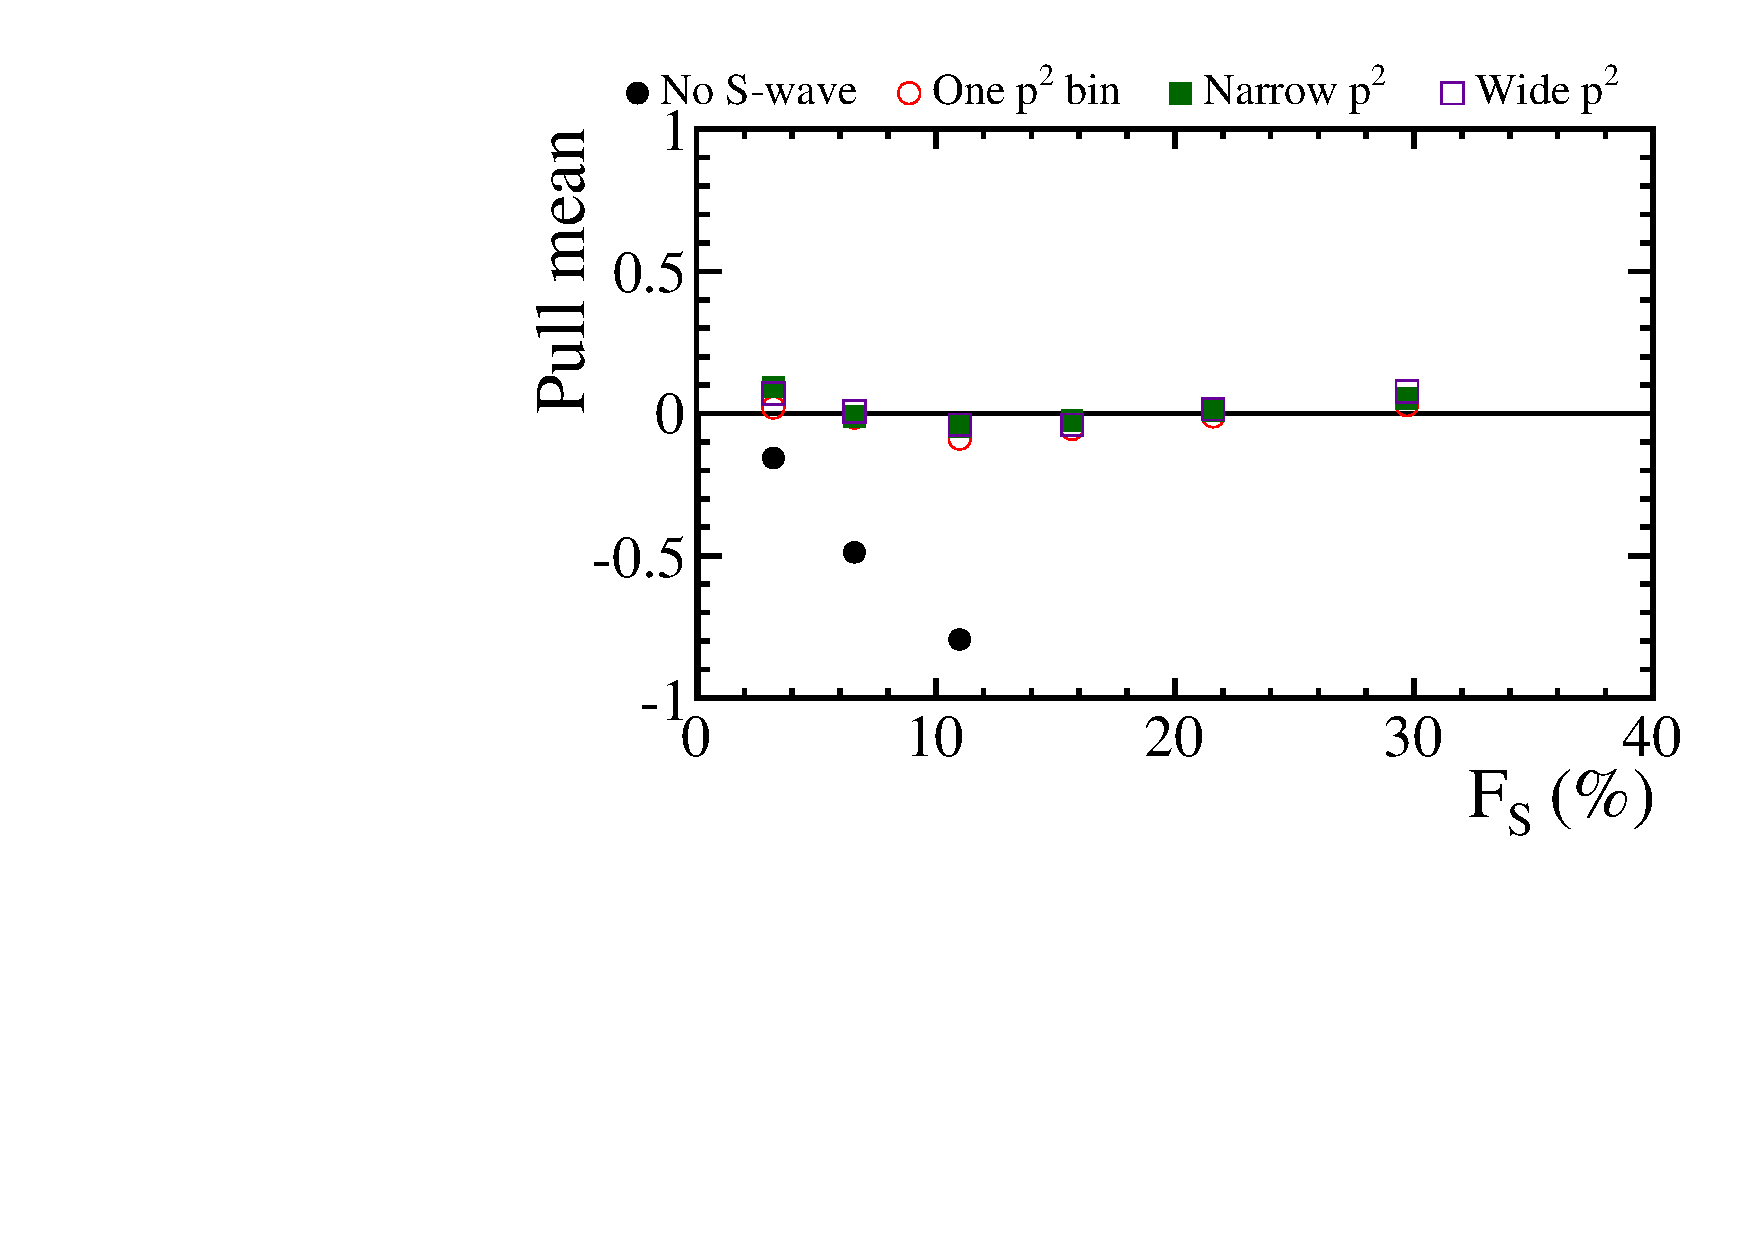
\includegraphics[width=0.48\textwidth]{chapter6/figs/fit_result_combo_fs_fl_mean.pdf}}
\subfigure[\AT2 ]{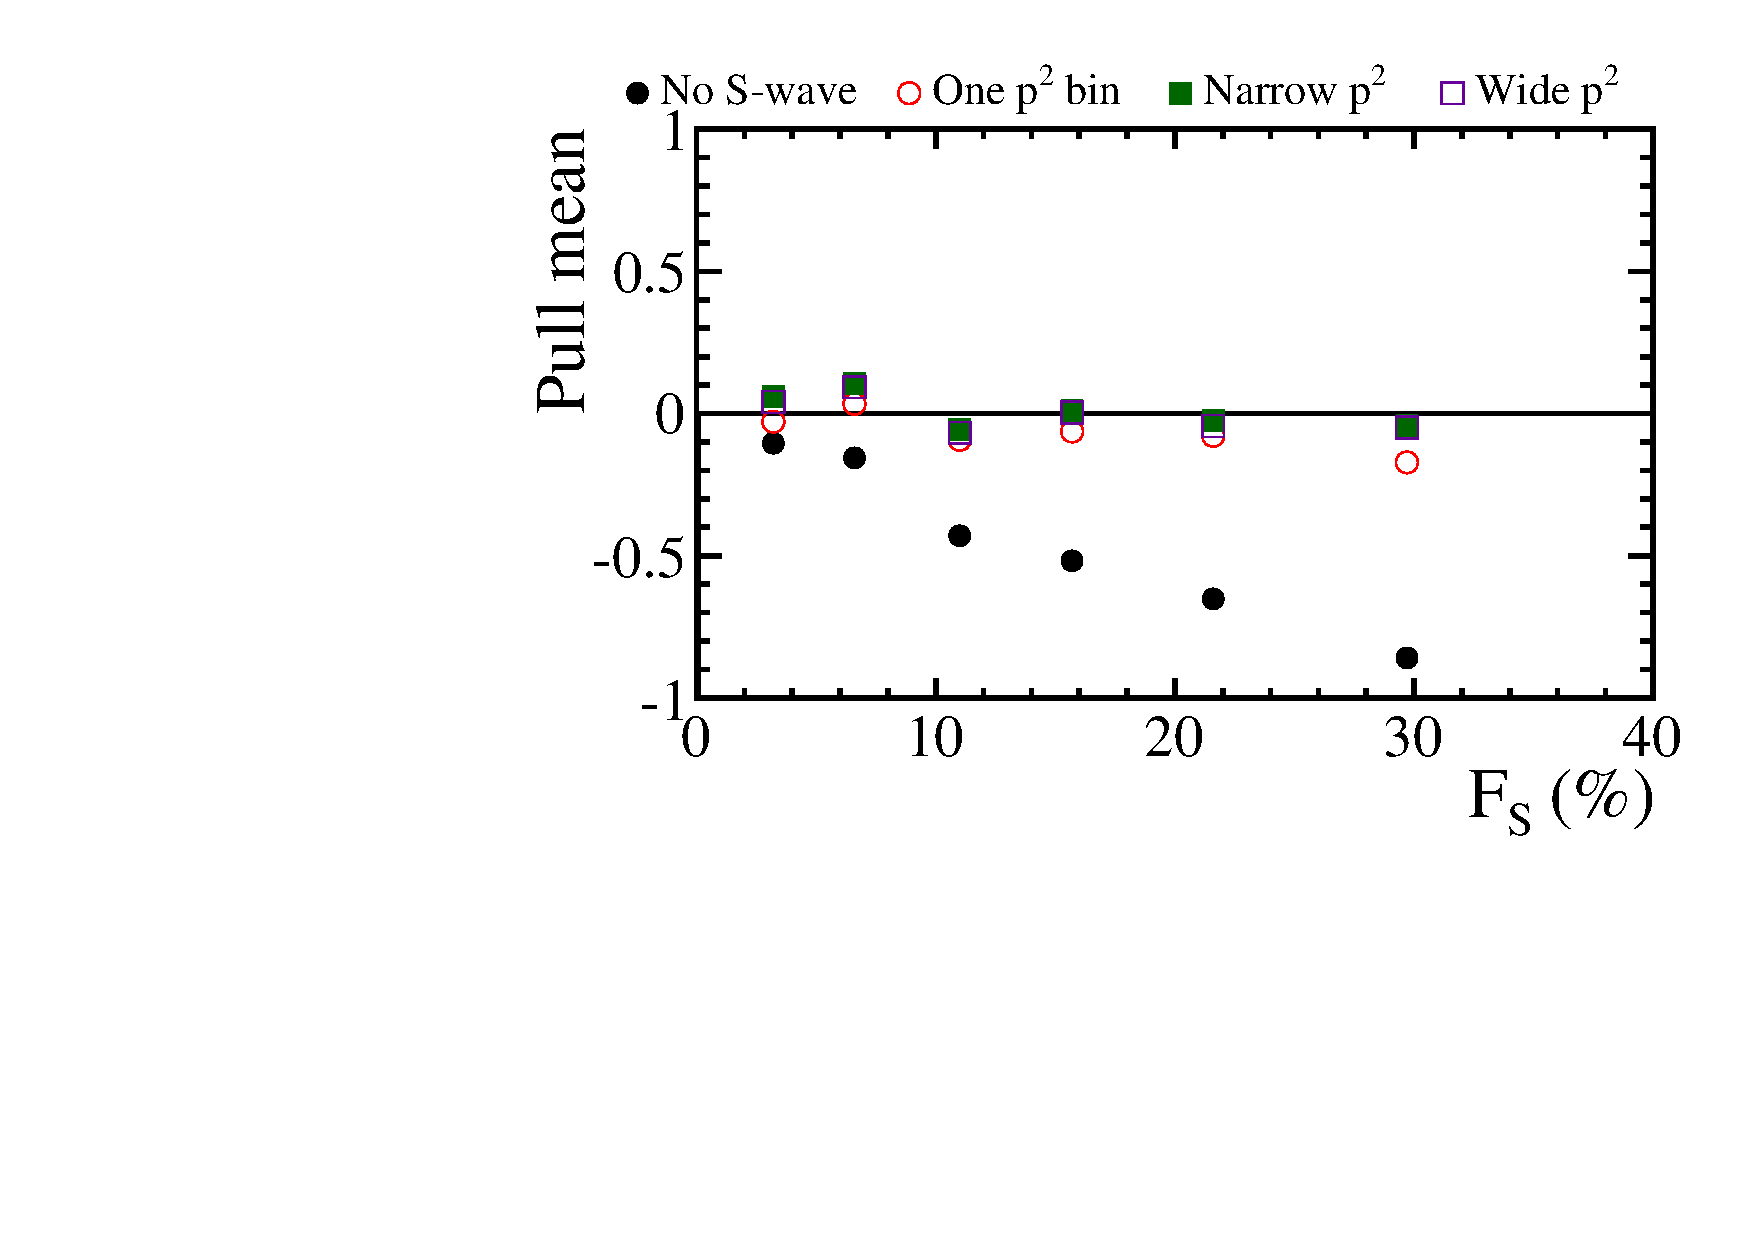
\includegraphics[width=0.48\textwidth]{chapter6/figs/fit_result_combo_fs_at2_mean.pdf}}
\subfigure[\AIm]{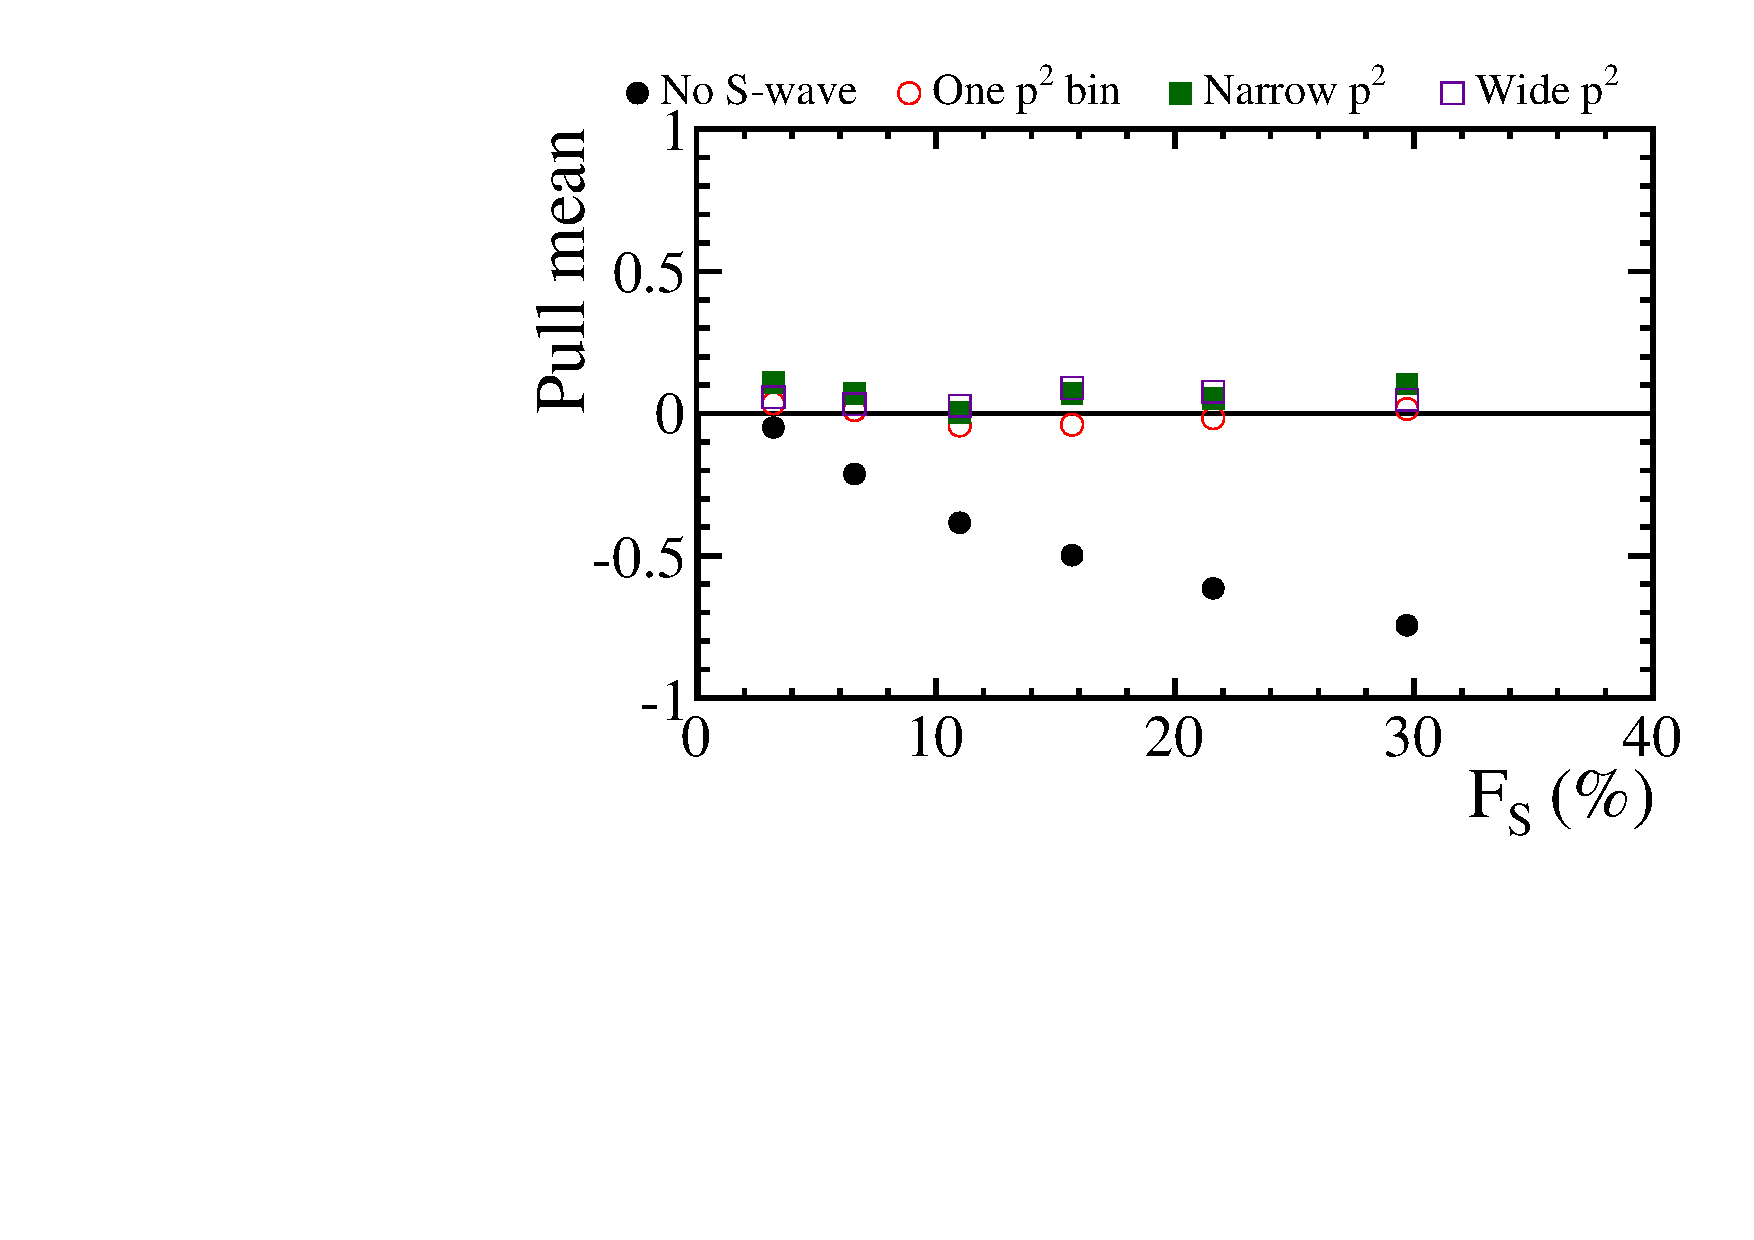
\includegraphics[width=0.48\textwidth]{chapter6/figs/fit_result_combo_fs_aim_mean.pdf}}
\caption[ Pull mean for the three different  
methods to incorporate the S-wave and when the S-wave 
is ignored.    ]
{Pull mean for the three different  
methods to incorporate the S-wave and when the S-wave 
is ignored. There is a slight shift when the S-wave is 
included for datasets of less than 200 events but this is removed from  all the observables 
when the S-wave is included in the fit 
for datasets of over 500 events. ~\label{fig:combofs}}
\end{figure}
The pull width  as a function of S-wave contribution 
for all three fit methods is shown in Fig.~\ref{fig:combofswidth}.
\begin{figure}[tb]
\centering
\subfigure[\AFB]{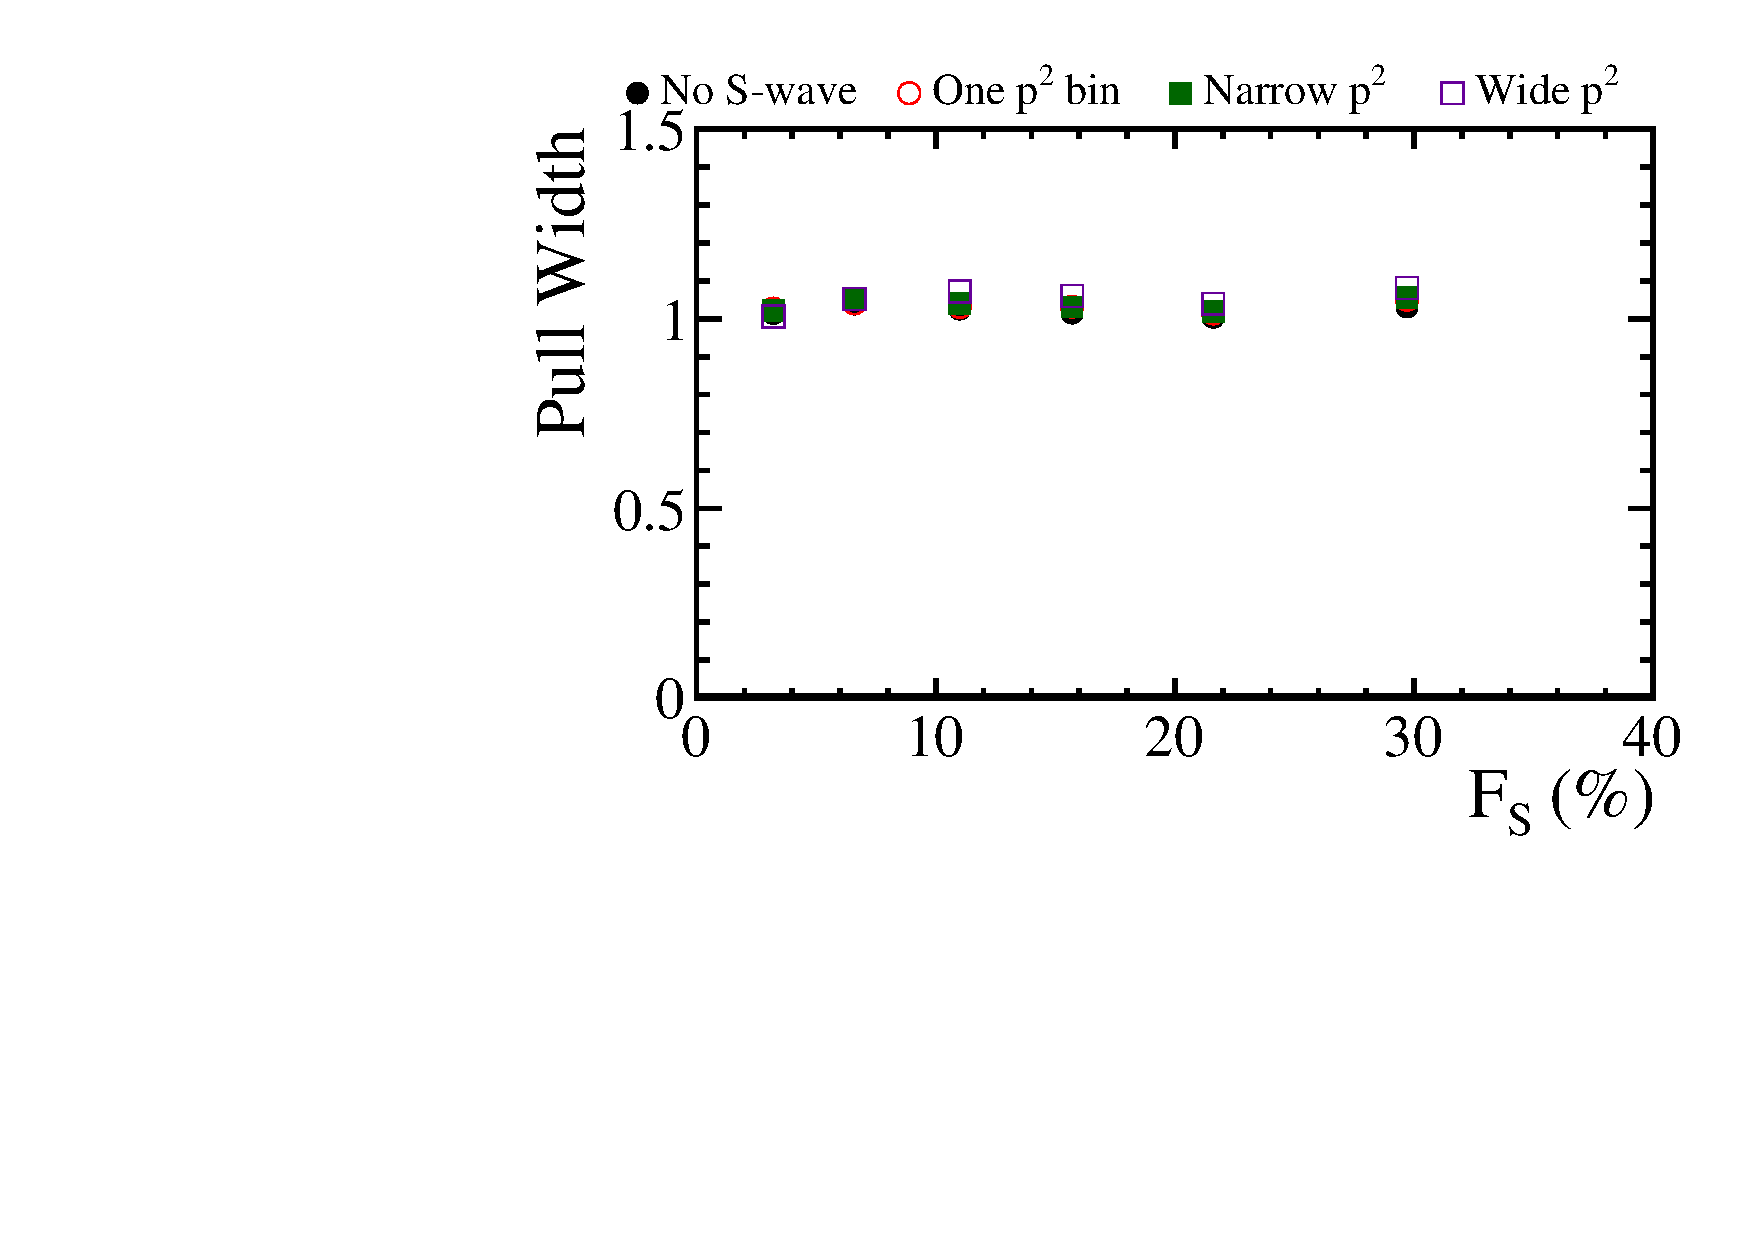
\includegraphics[width=0.48\textwidth]{chapter6/figs/fit_result_combo_fs_afb_width.pdf}}
\subfigure[\FL]{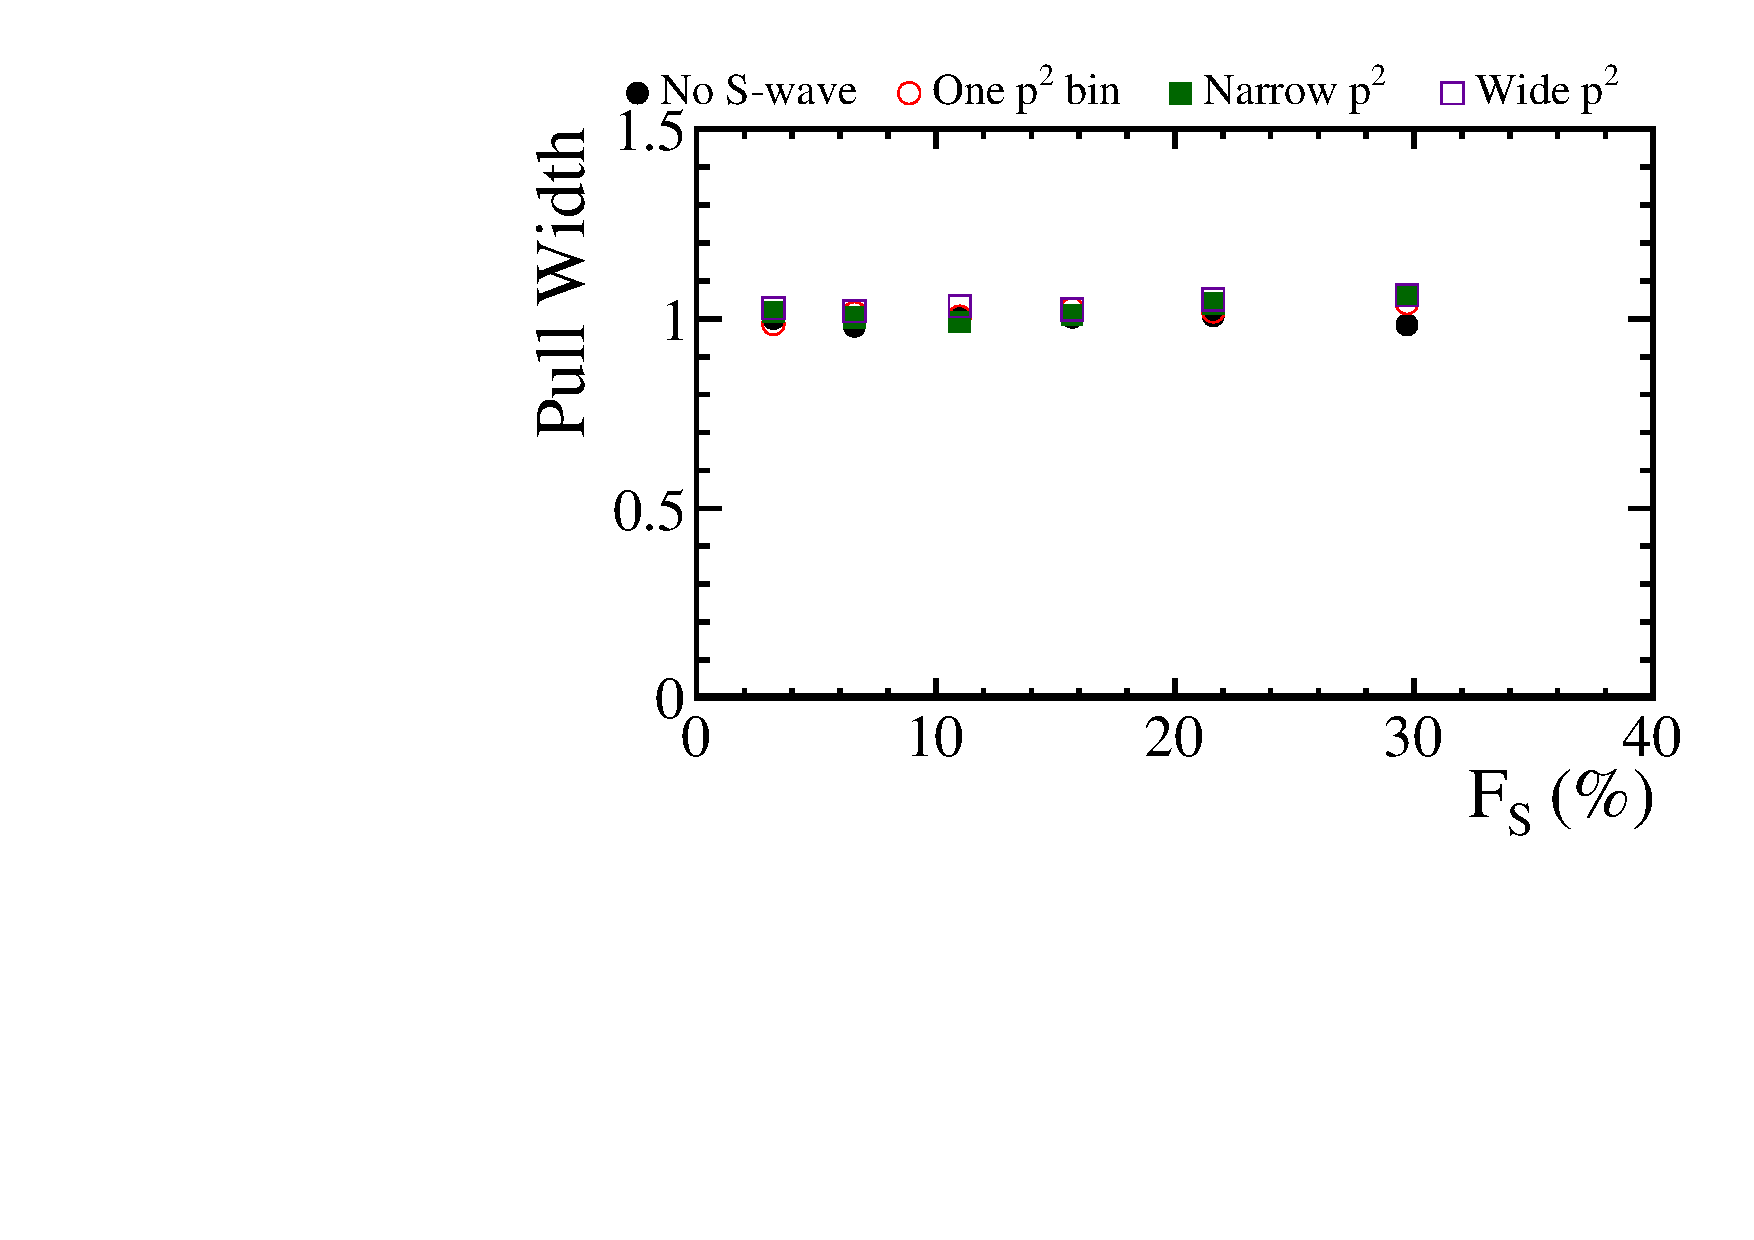
\includegraphics[width=0.48\textwidth]{chapter6/figs/fit_result_combo_fs_fl_width.pdf}}
\subfigure[\AT2 ]{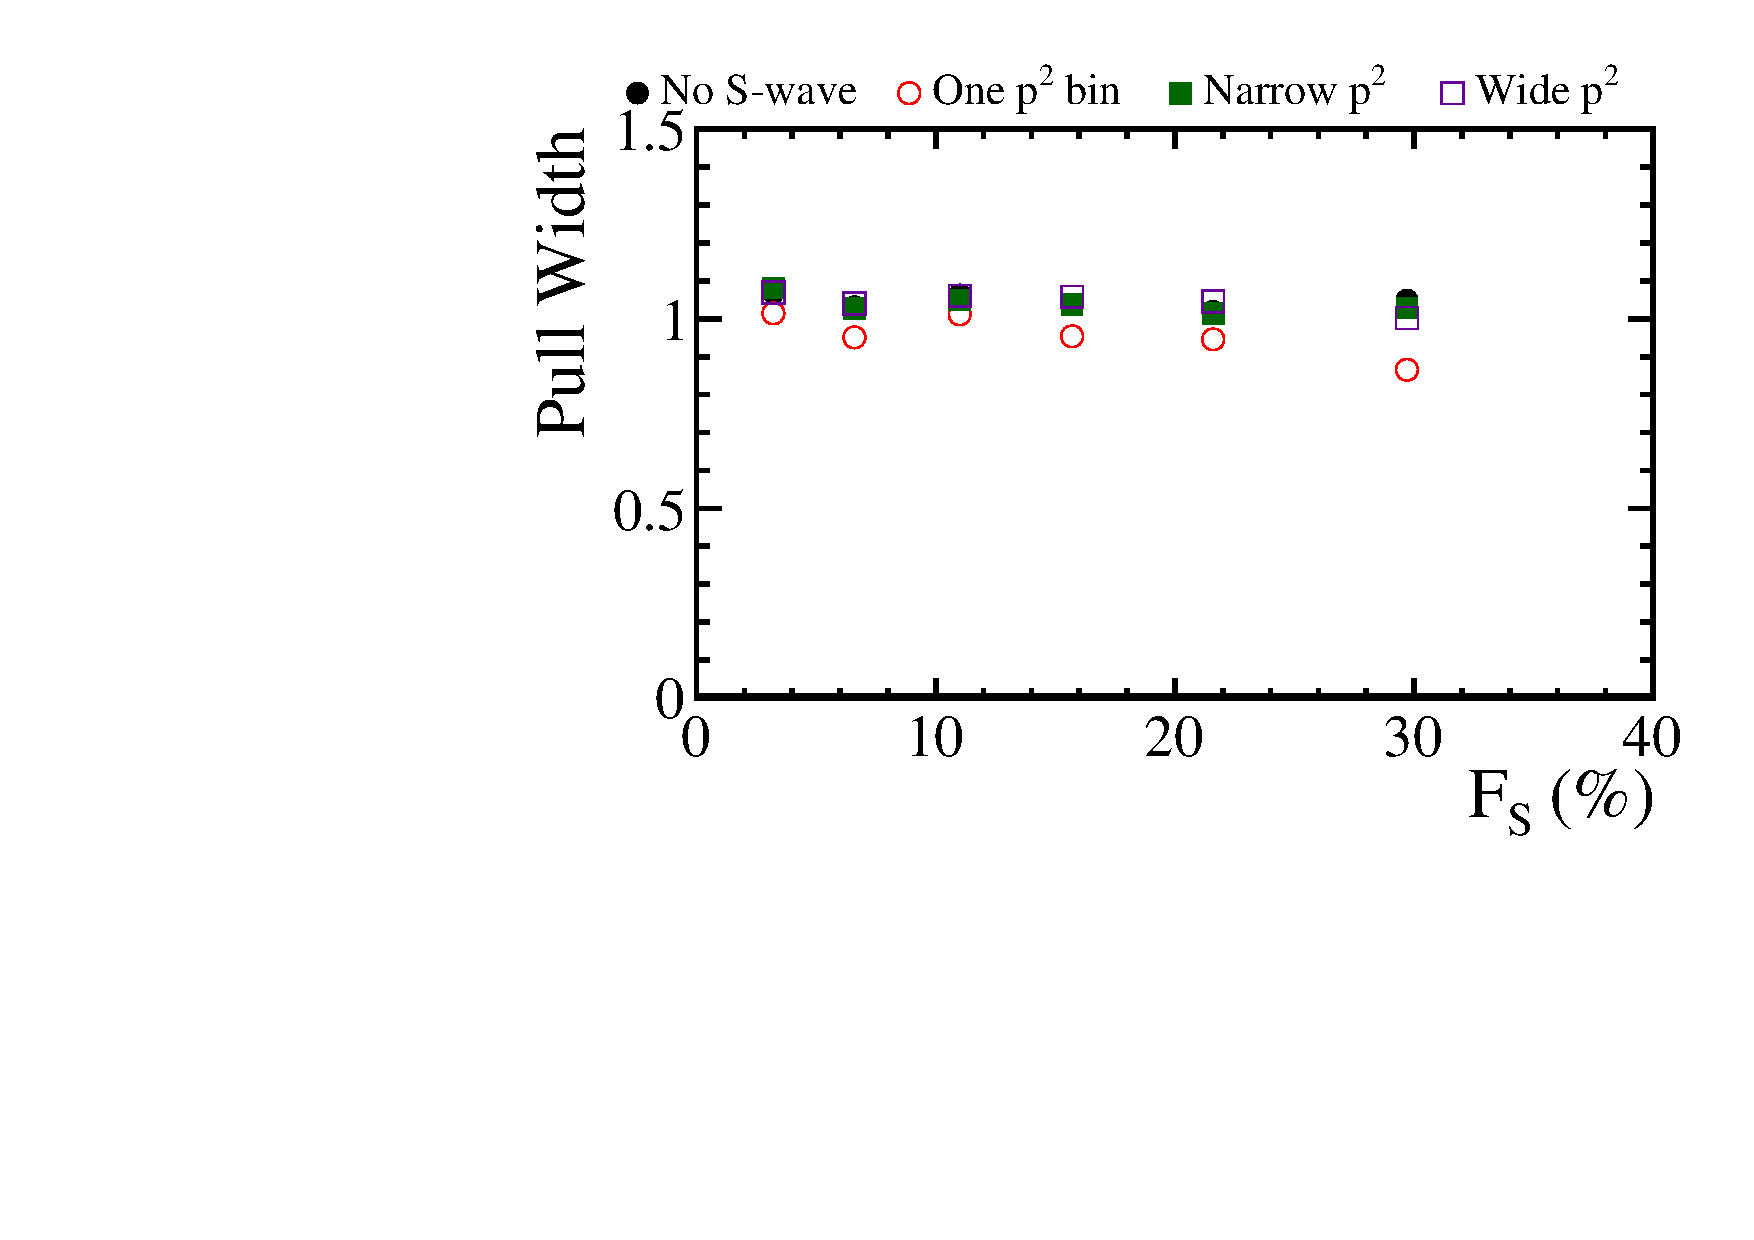
\includegraphics[width=0.48\textwidth]{chapter6/figs/fit_result_combo_fs_at2_width.pdf}}
\subfigure[\AIm]{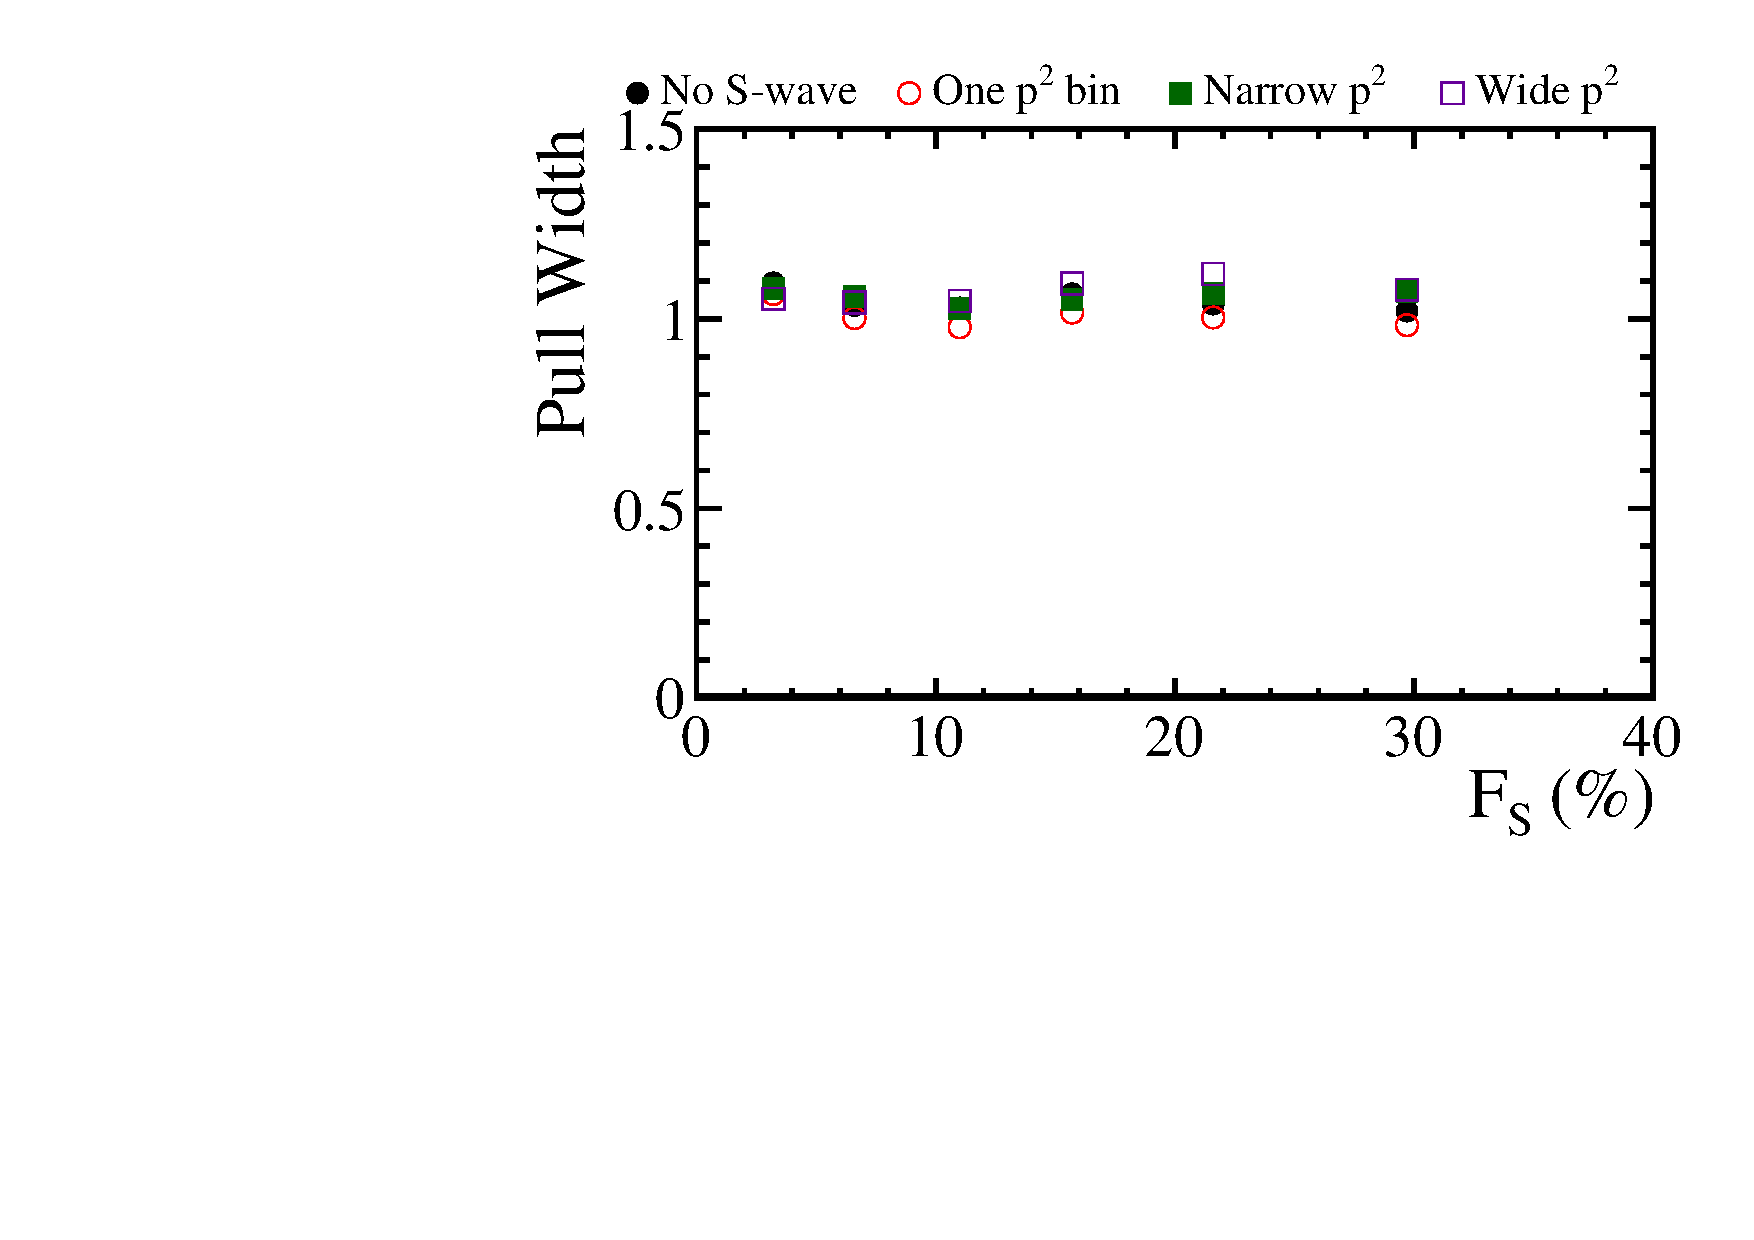
\includegraphics[width=0.48\textwidth]{chapter6/figs/fit_result_combo_fs_aim_width.pdf}}
\caption[ Pull width for the three different  
methods to incorporate the S-wave and when the S-wave 
is ignored.    ]
{Pull width for the three different  
methods to incorporate the S-wave and when the S-wave 
is ignored. There is a slight shift when the S-wave is 
included for datasets of less than 200 events but this is removed from  all the observables 
when the S-wave is included in the fit 
for datasets of over 500 events. ~\label{fig:combofswidth}}
\end{figure}





\section{Systematic test}
\label{sec:swave:isobar}

The results shown in Figs.~\ref{fig:combods} and~\ref{fig:combofs} could
 have an implicit model dependence through the use of the LASS parametrisation to model the \psq spectrum.
 In order to understand the size of this effect, the measurements were repeated using an isobar
model to parametrise the \kpi S-wave as in Ref.~\cite{PhysRevLett.89.121801}.
In the isobar model the S-wave is described as a simple sum of functions for the $\Kstarzz(1430)$ 
and the $\kappa(800)$ along with a constant non-resonant term,
\begin{align}
T_I(\psq) &= N_{\kappa} \mathcal{F}_{\kappa}(\psq) \exp(\phi_{\kappa}) + N_S \mathcal{F}_S(\psq) \exp(\phi_S)  + NR
\end{align}
where $N_i$ is the normalisation for each contribution and $\phi_i$ is the phase of each contribution.
The $\Kstarzz(1430)$ is described by a relativistic Breit-Wigner function as in the LASS parametrisation,
\begin{align}
\mathcal{F}_S(\psq) &= \cot\delta_S = \frac{ \psq - m_{\mathrm{S}}^2 }{ \Gamma_{\mathrm{S}}(\psq) m_{\mathrm{S}}}.
\end{align}
and the $\kappa(800)$ is described similarly
\begin{align}
\mathcal{F}_{\kappa}(\psq) &= \cot\delta_{\kappa} = \frac{ \psq - m_{\kappa}^2 }{ \Gamma_{\kappa}(\psq) m_{\kappa}  }.
\end{align}
where the mass and width of the $\kappa(800)$ are taken from Ref.~\cite{PDG2012}.
The existence of the $\kappa(800)$ is under debate with no conclusive evidence.
The amplitude $T_I$ is normalised such that it has the same integral as the LASS amplitude ($T_S$) 
over the \psq range from threshold to an upper limit of 2.5\gevgevcccc. 
This limit is chosen to encompass most of resonant $\Kstarzz(1430)$.
The \psq spectrum of the combined P wave and the two S-wave models is shown in Fig.~\ref{fig:spwave:isobar}.
\begin{figure}[tb]
\centering
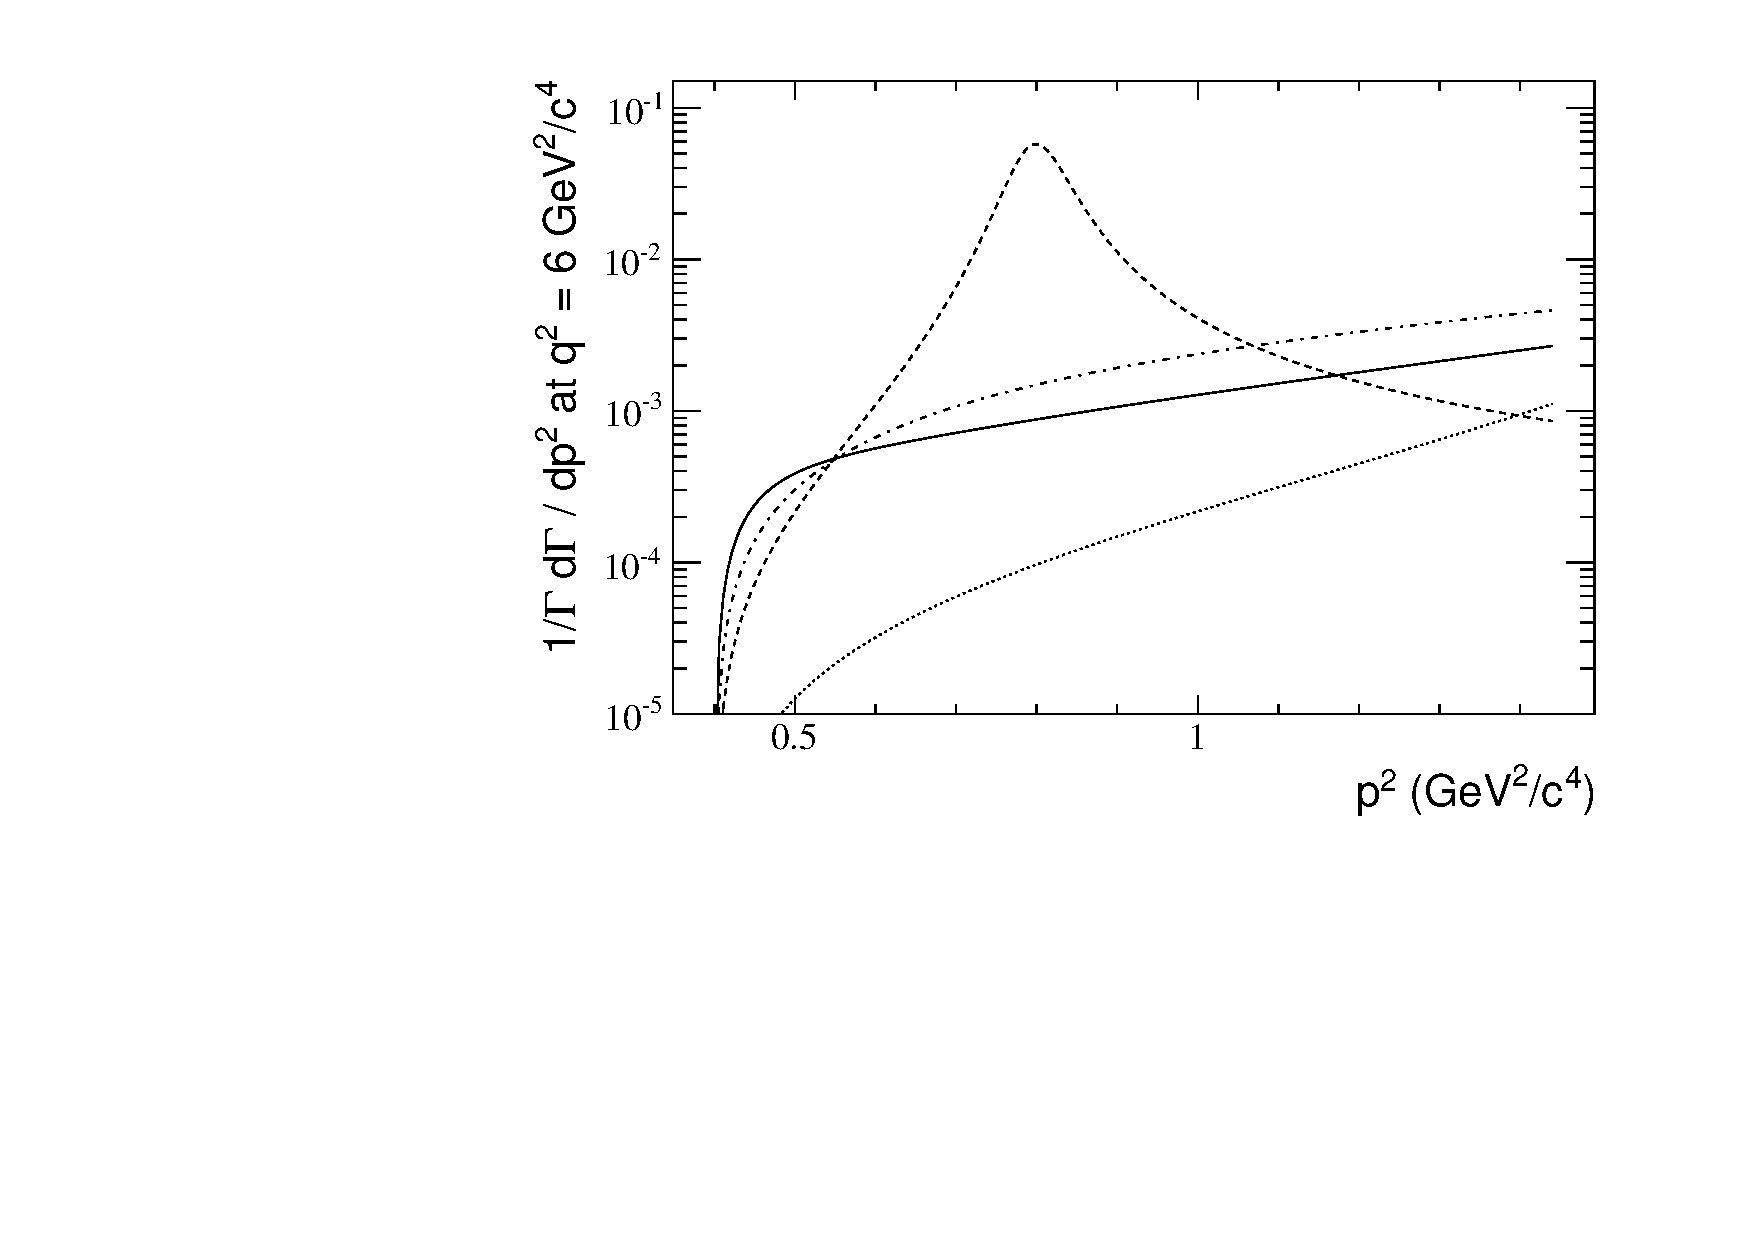
\includegraphics[width=0.66\textwidth]{chapter6/figs/calc_isobar_psq_branch_frac_logy.pdf}
\caption{ An illustration of the \psq spectrum for the P-wave (solid) and the
 isobar S-wave (dashed) and the LASS S-wave (dash-dotted) and the D-wave (dotted). 
~\label{fig:spwave:isobar} } 
\end{figure}

The model-dependence of the \psq spectrum was tested by generating events where an isobar model was used for 
the S-wave contribution and fitting the angular distribution using the LASS parametrisation.
The relative resolution between the results obtained when generating with the 
LASS parametrisation and the results obtained when generating with an isobar model
are shown in Fig.~\ref{fig:ratio:isobar}.
\begin{figure}[tb]
\centering
\subfigure[\AFB]{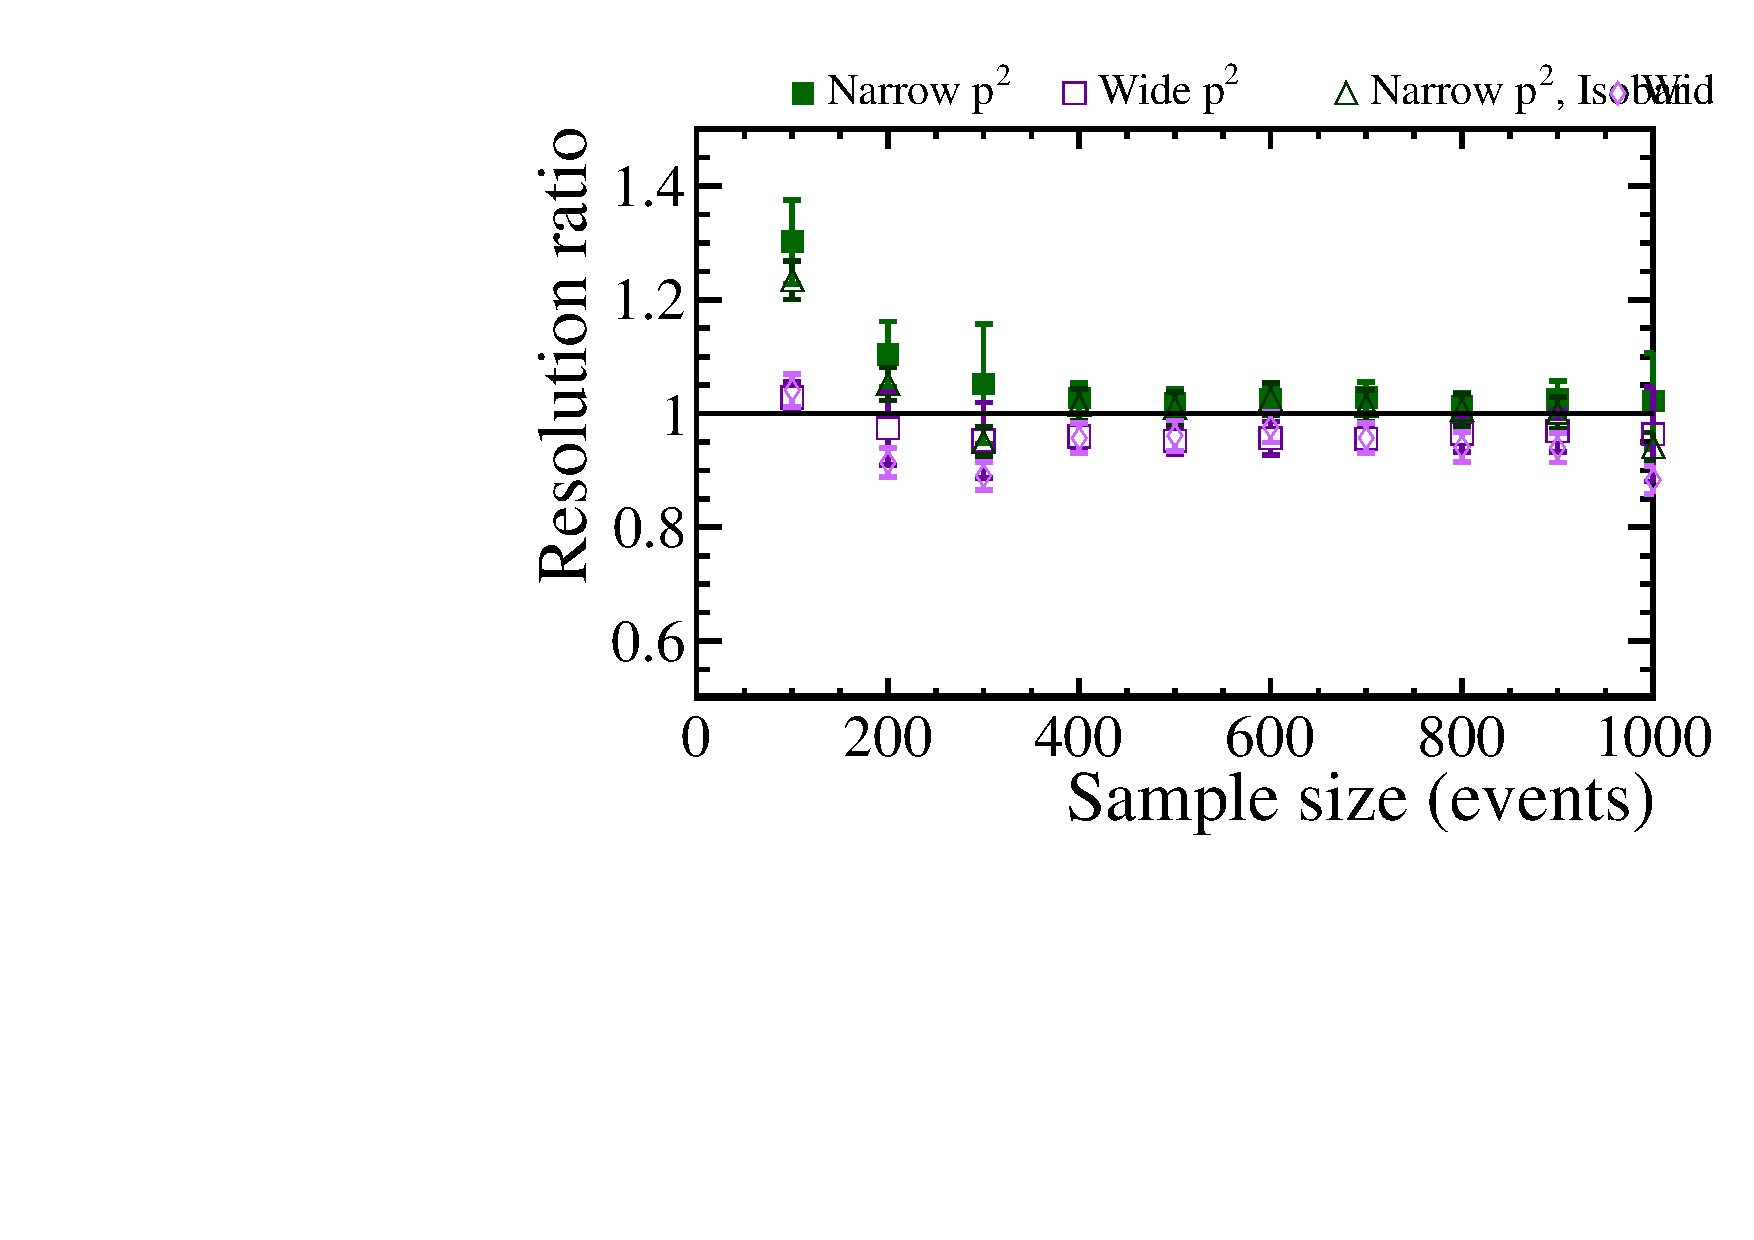
\includegraphics[width=0.48\textwidth]{chapter6/figs/fit_result_ratio_ds_isobar_afb_res.pdf}}
\subfigure[\FL]{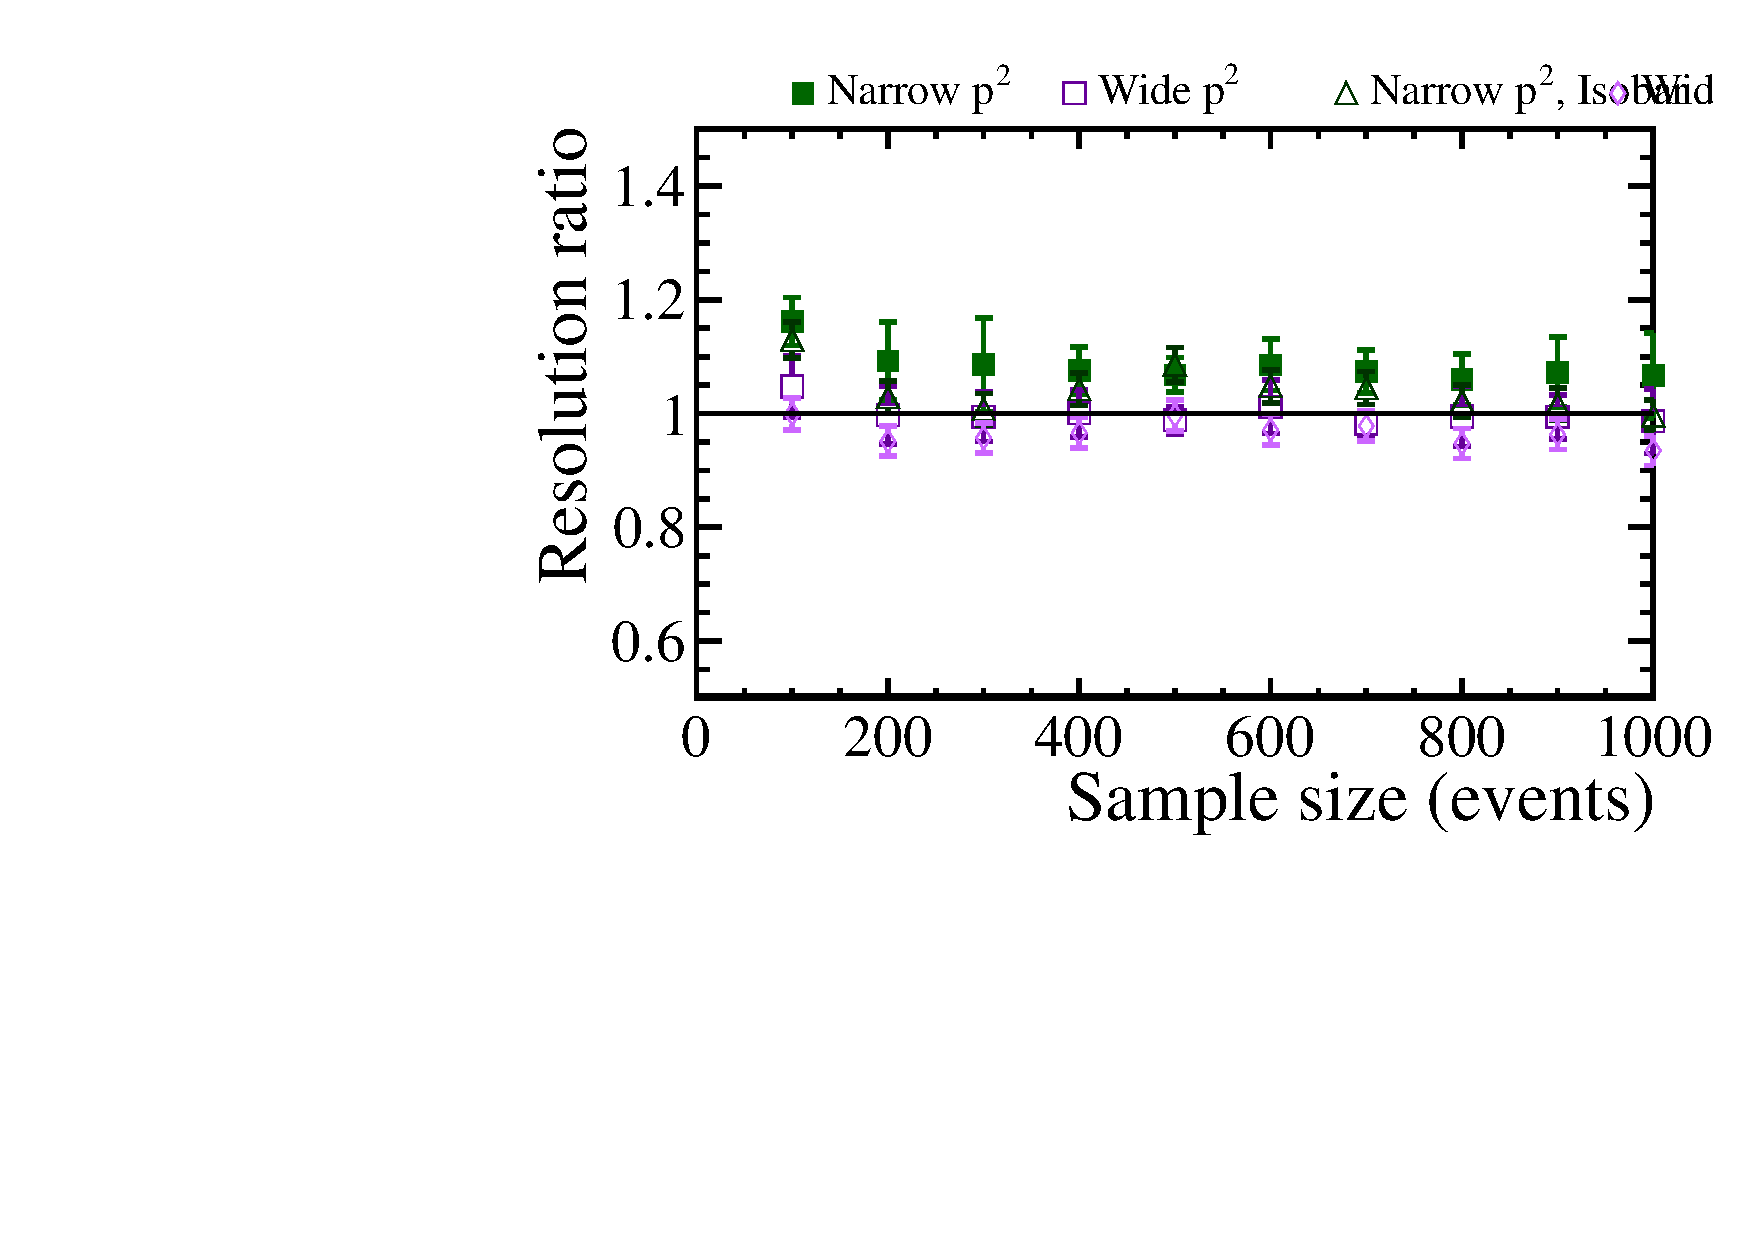
\includegraphics[width=0.48\textwidth]{chapter6/figs/fit_result_ratio_ds_isobar_fl_res.pdf}}
\subfigure[\AT2 ]{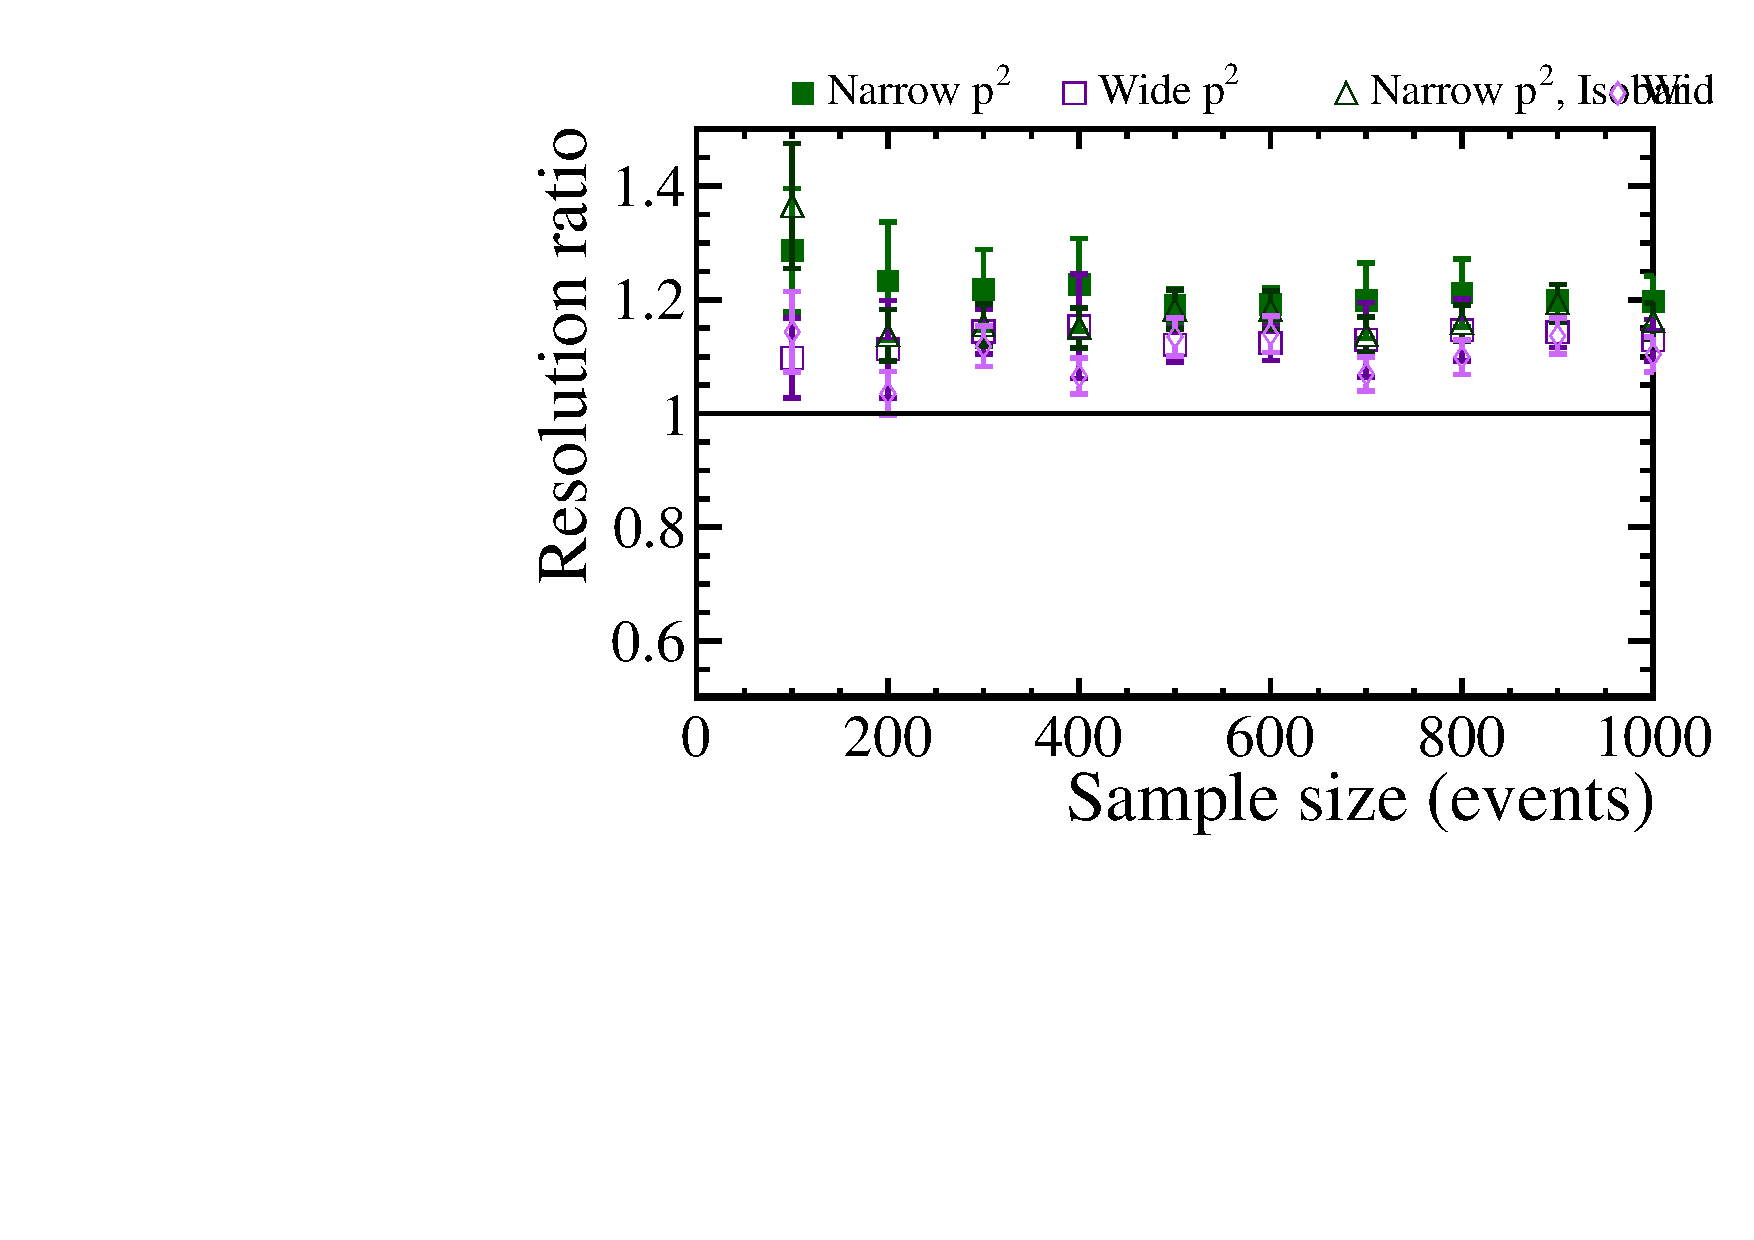
\includegraphics[width=0.48\textwidth]{chapter6/figs/fit_result_ratio_ds_isobar_at2_res.pdf}}
\subfigure[\AIm]{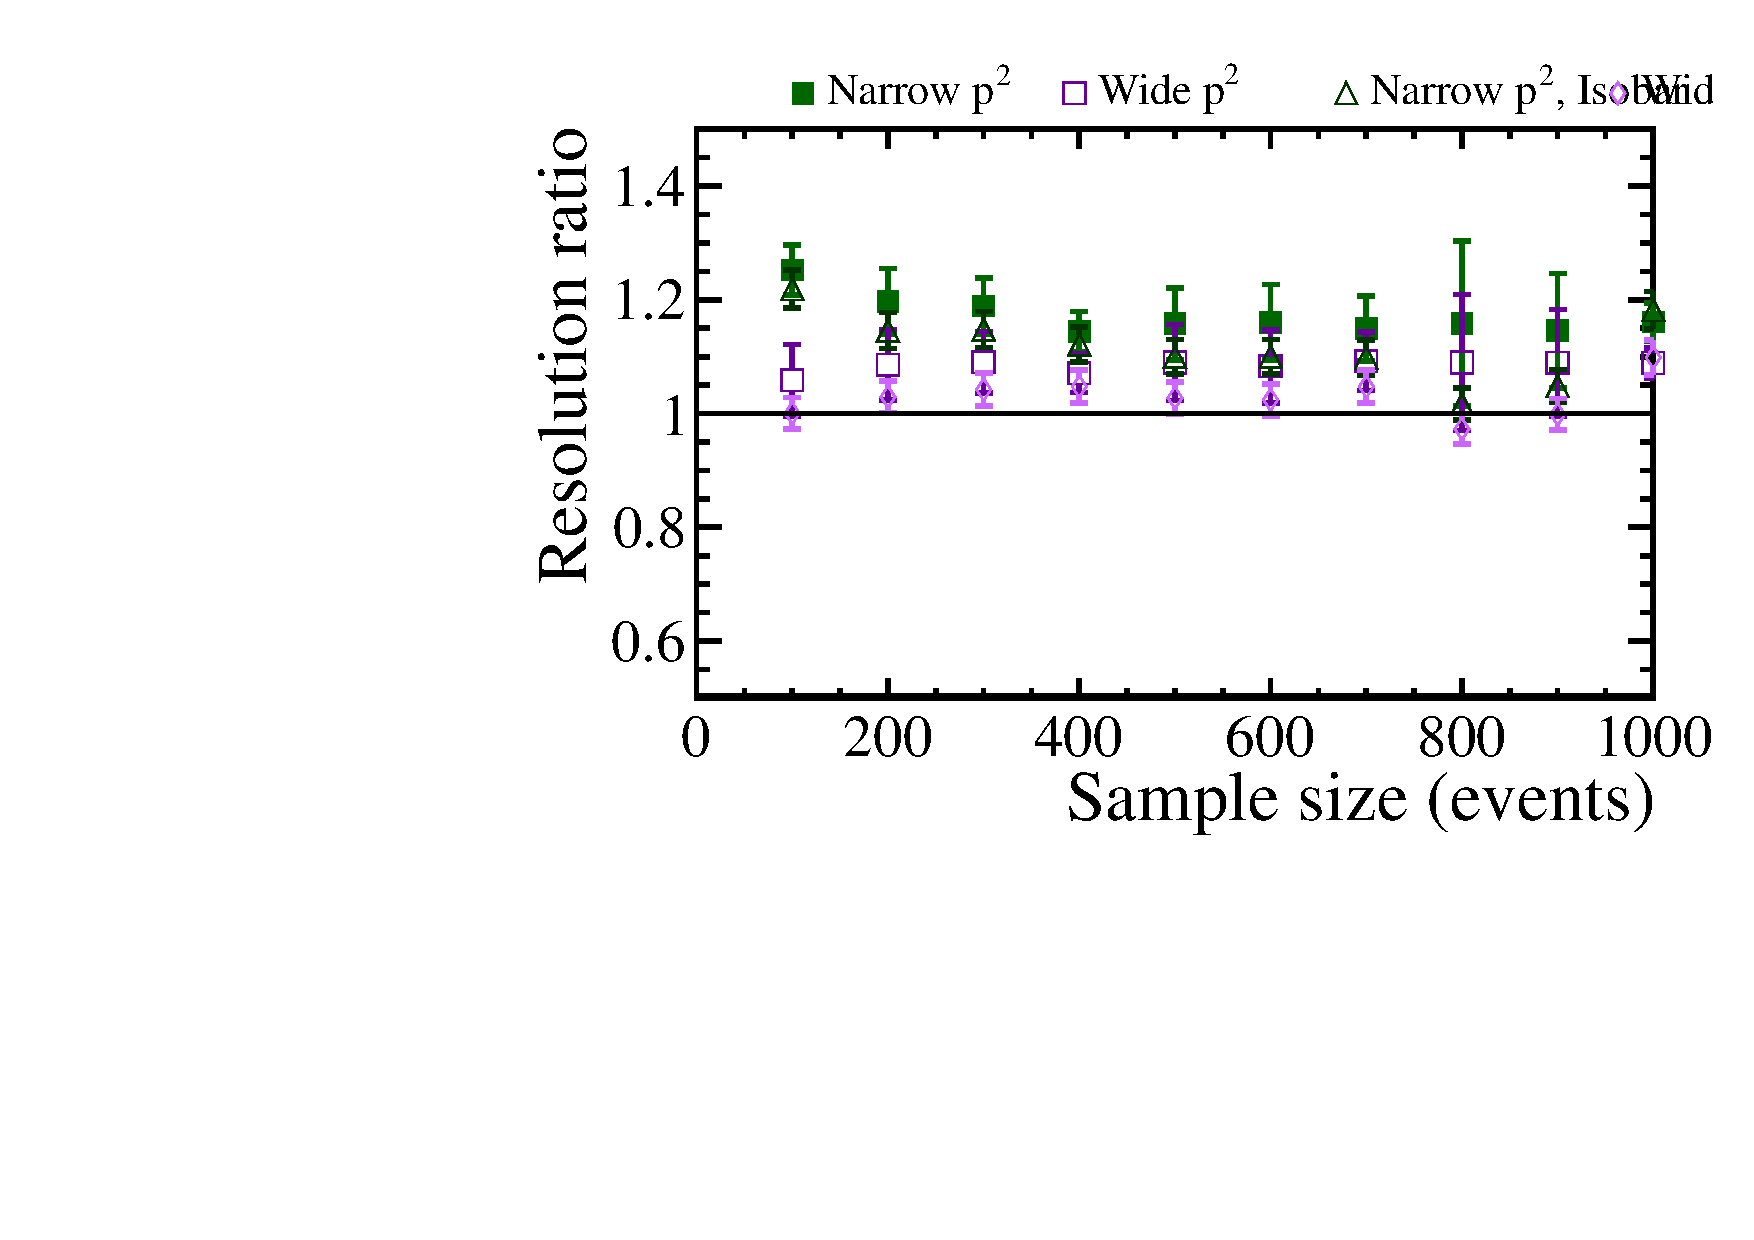
\includegraphics[width=0.48\textwidth]{chapter6/figs/fit_result_ratio_ds_isobar_aim_res.pdf}}
\caption[ Resolutions for three different methods to incorporate 
the S-wave relative to the resolution obtained when the S-wave is ignored.   ]
{Resolutions for three different methods to incorporate 
the S-wave relative to the resolution obtained when the S-wave is ignored. 
The S-wave has been generated using an isobar model. ~\label{fig:ratio:isobar}}
\end{figure}
The bias on the central values of the angular observables when the S-wave is ignored
as a function of the size of the dataset is shown in Fig.~\ref{fig:combods:isobar}.
\begin{figure}[tb]
\centering
\subfigure[\AFB]{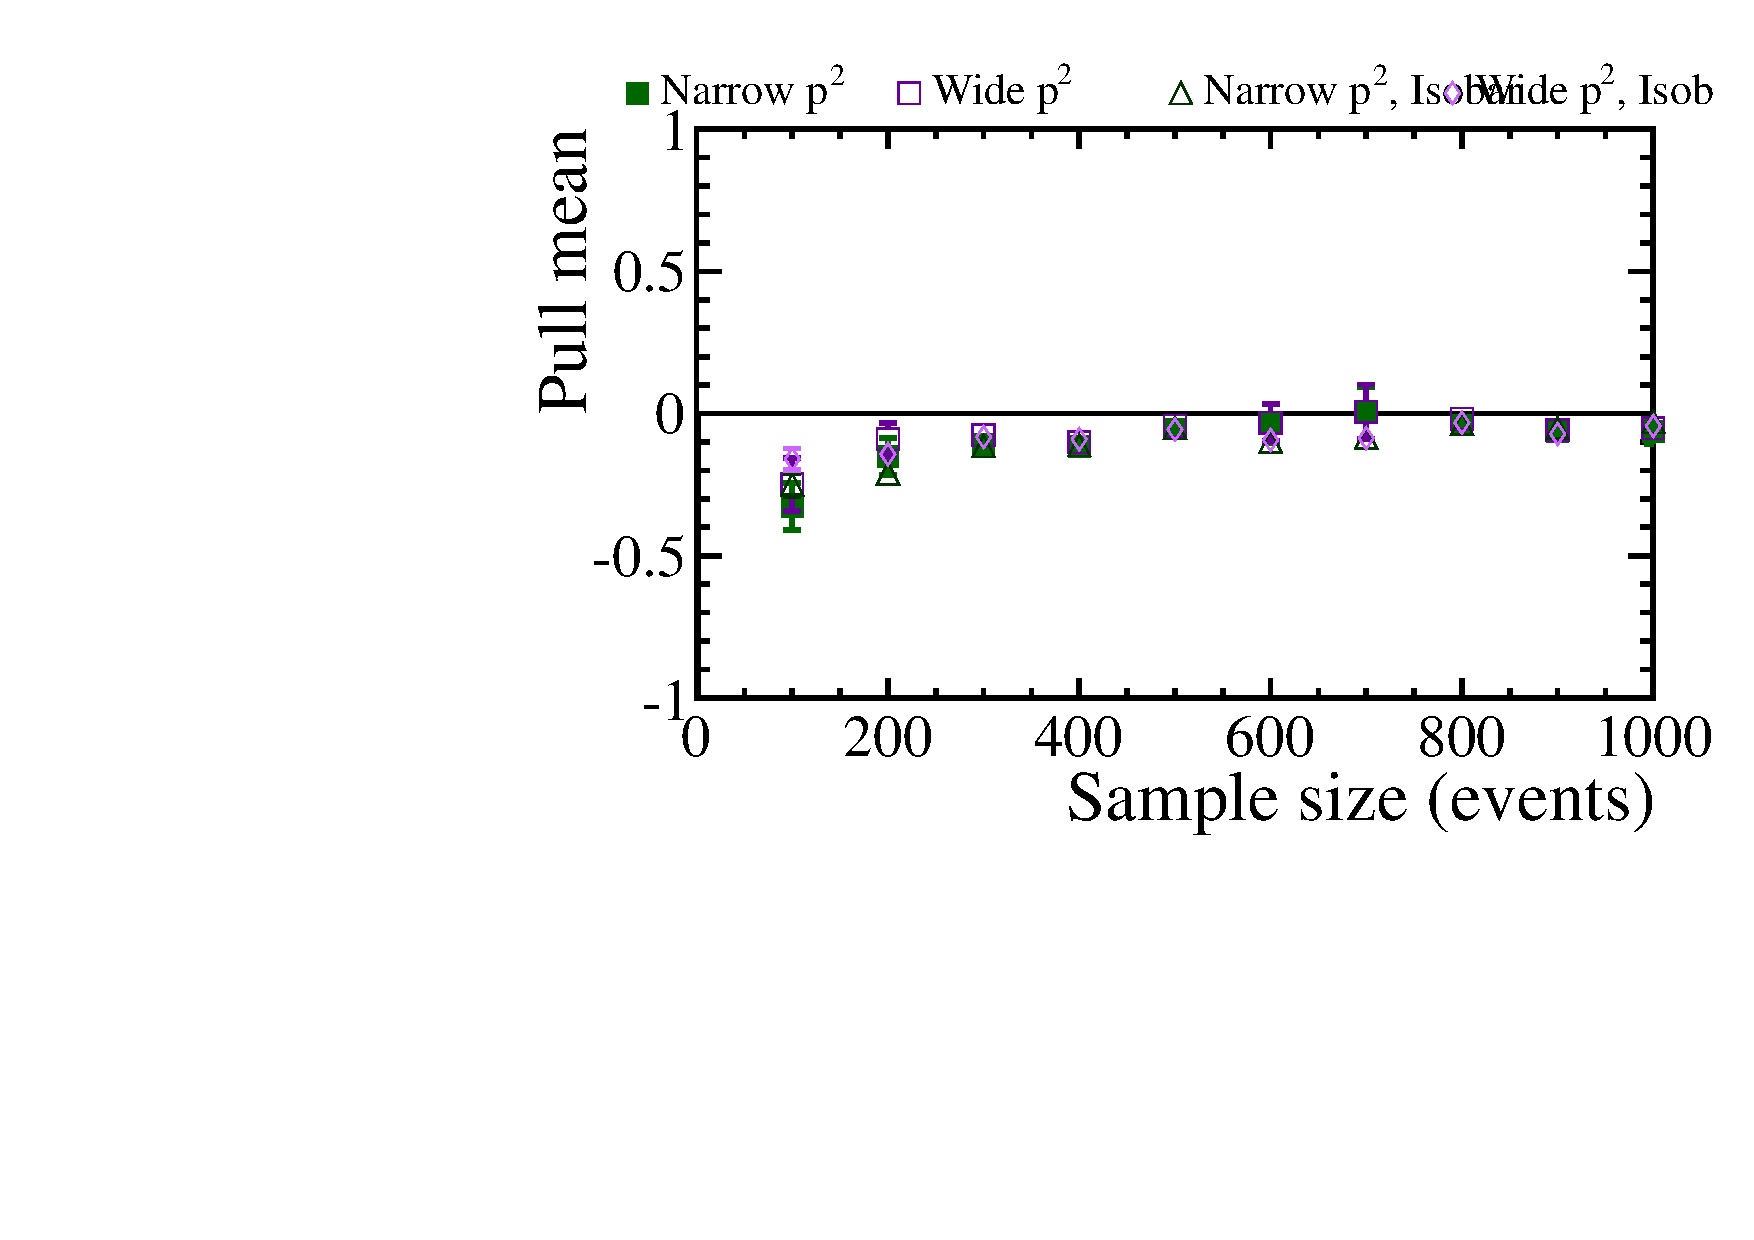
\includegraphics[width=0.48\textwidth]{chapter6/figs/fit_result_combo_ds_isobar_afb_mean.pdf}}
\subfigure[\FL]{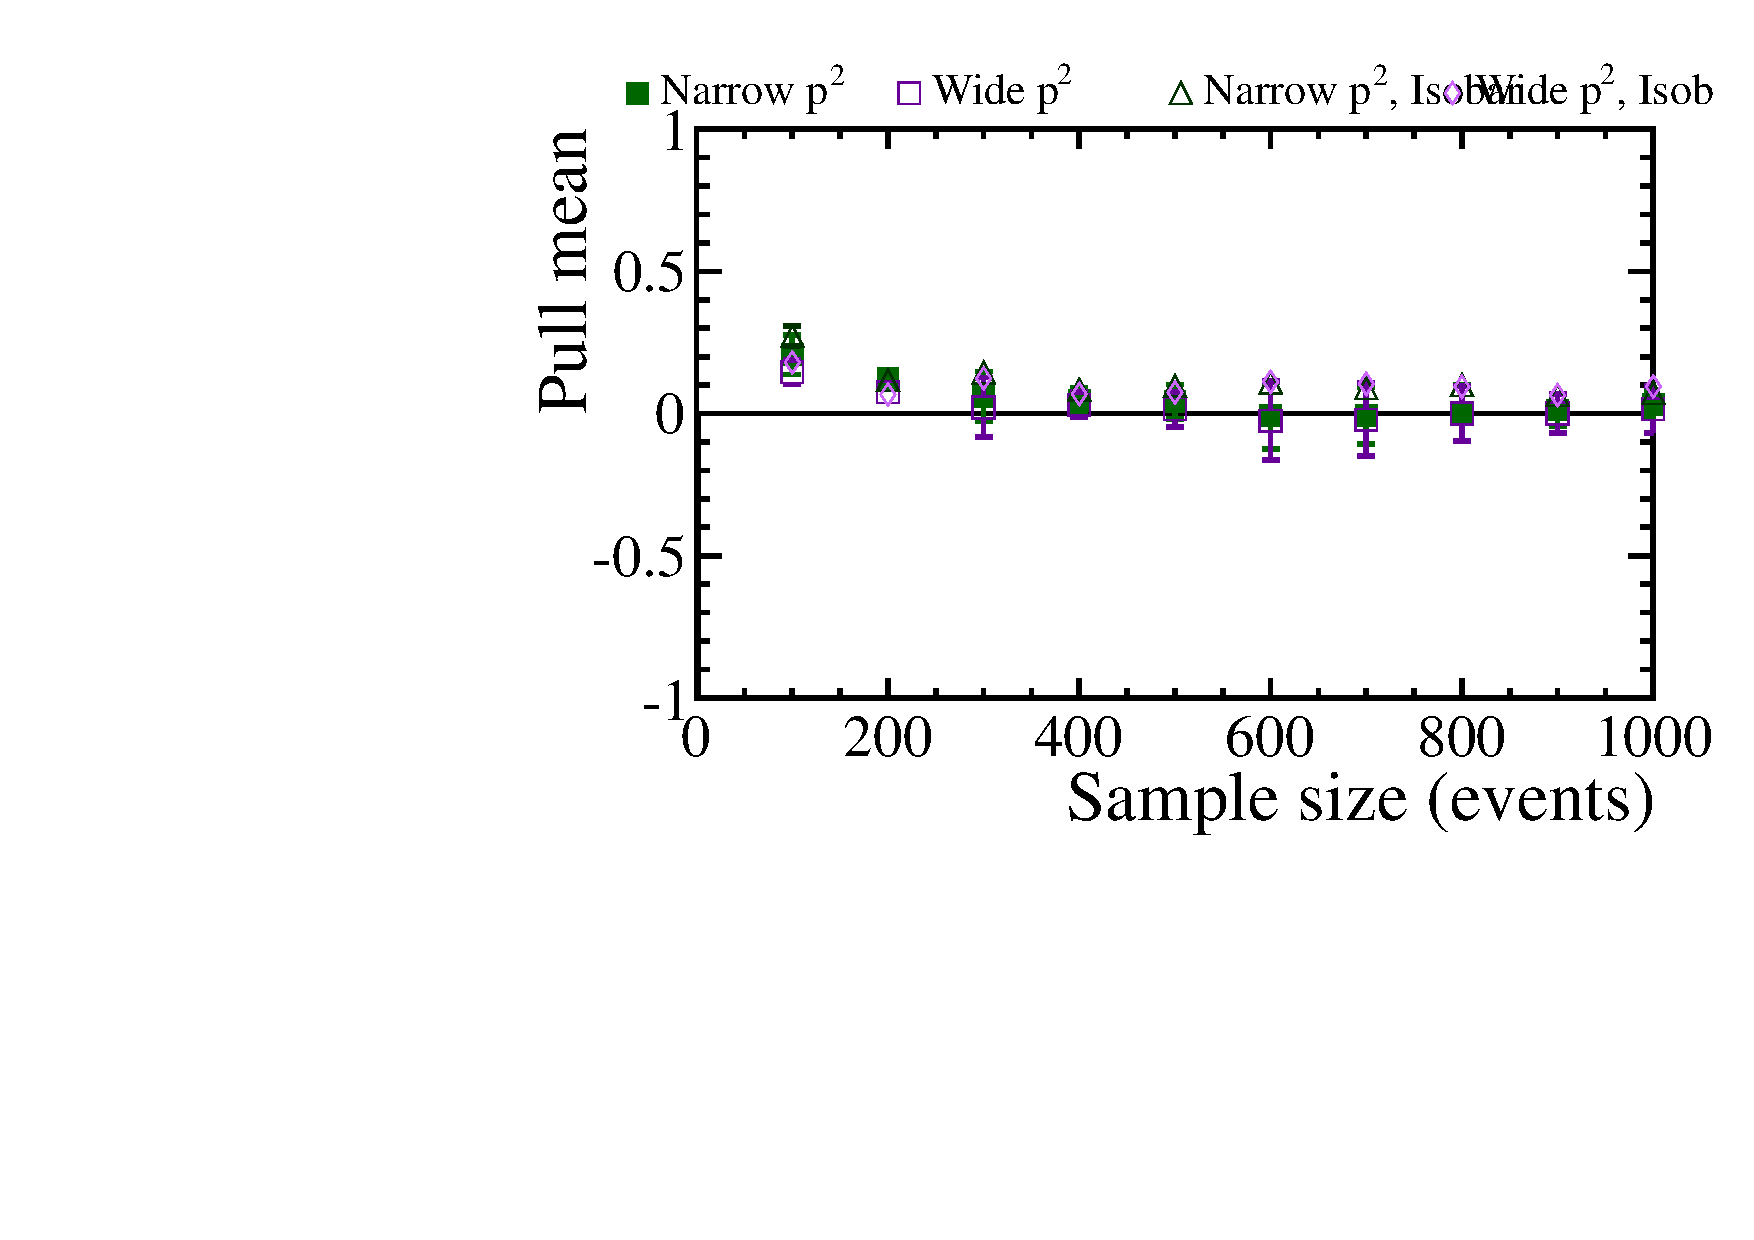
\includegraphics[width=0.48\textwidth]{chapter6/figs/fit_result_combo_ds_isobar_fl_mean.pdf}}
\subfigure[\AT2 ]{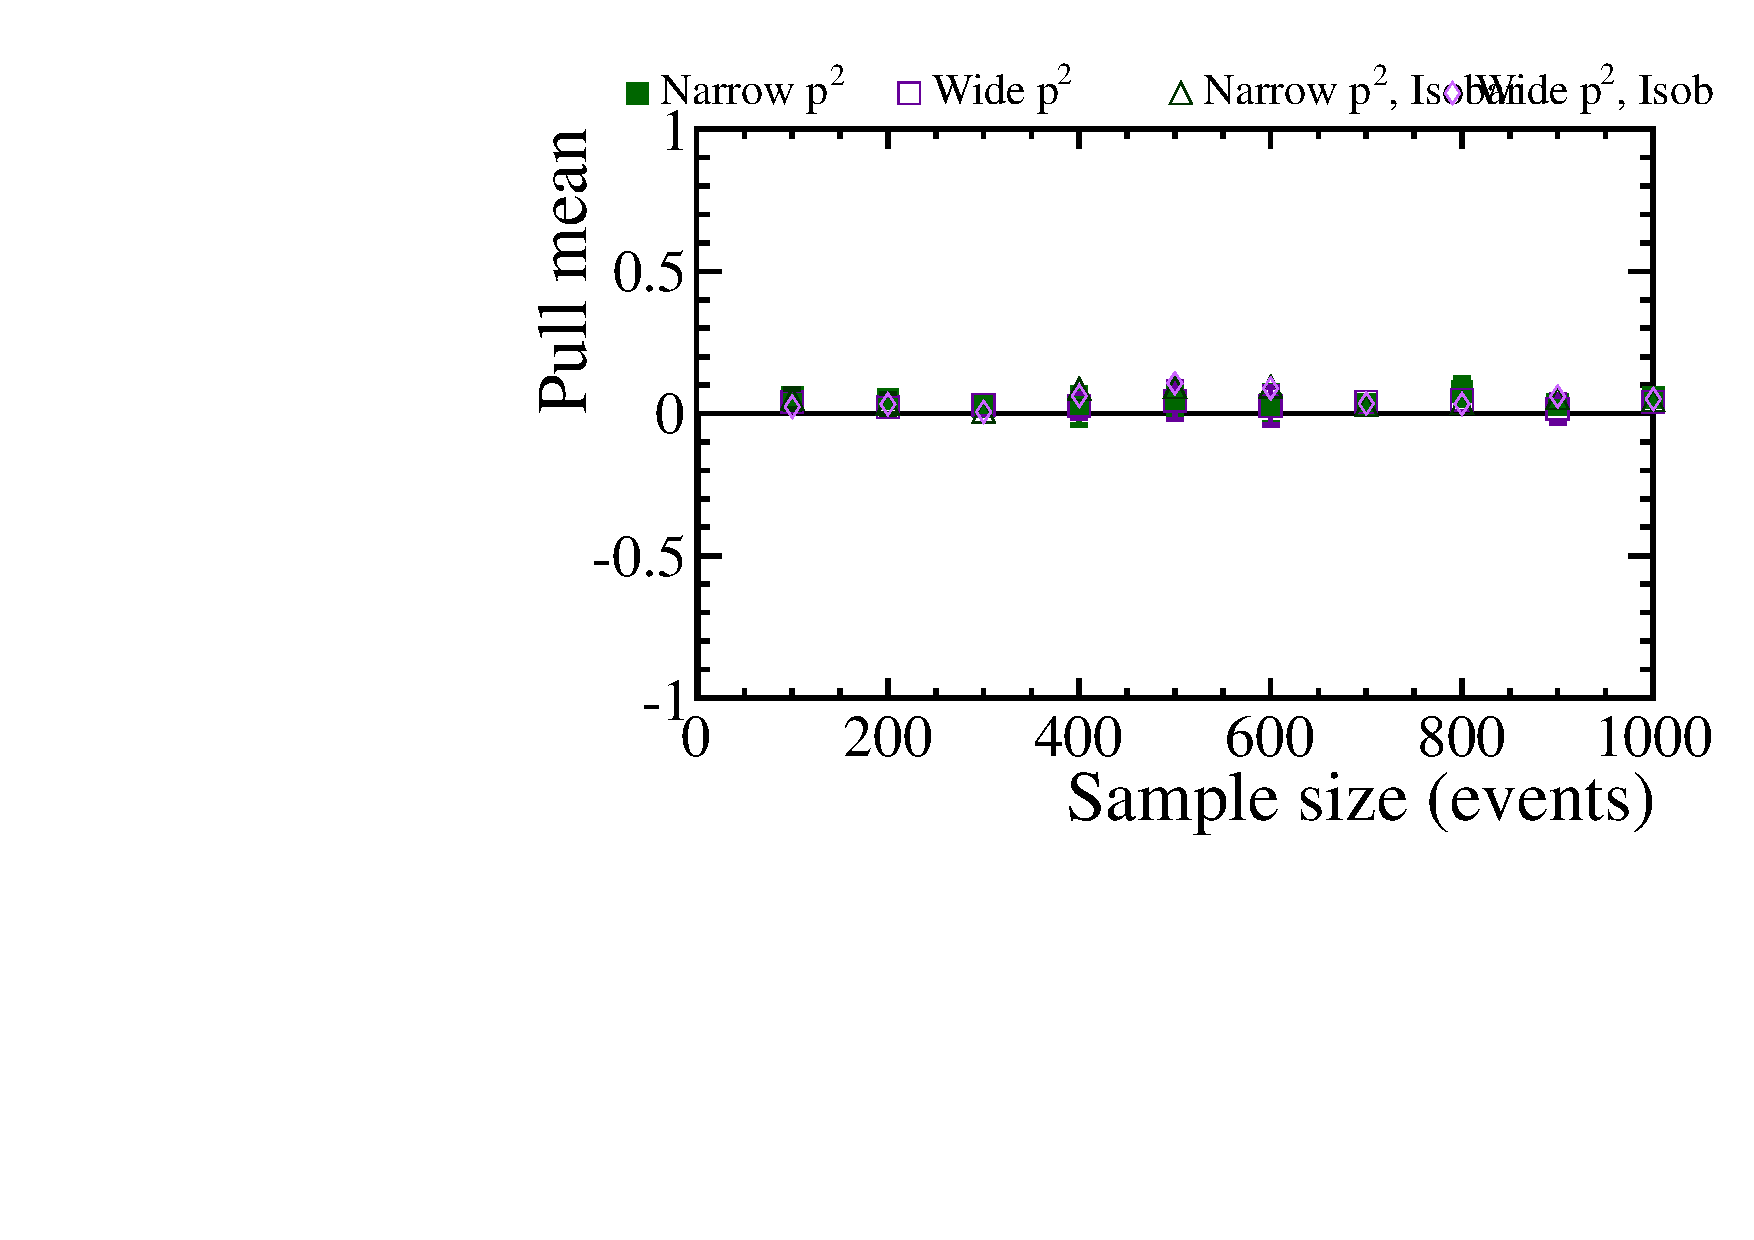
\includegraphics[width=0.48\textwidth]{chapter6/figs/fit_result_combo_ds_isobar_at2_mean.pdf}}
\subfigure[\AIm]{\includegraphics[width=0.48\textwidth]{chapter6/figs/fit_result_combo_ds_isobar_aim_mean.pdf}}
\caption[ Pull mean for the three different  
methods to incorporate the S-wave and when the S-wave 
is ignored.      ]
{Pull mean for the three different  
methods to incorporate the S-wave and when the S-wave 
is ignored. 
The S-wave has been generated using an isobar model.
 There is a slight shift when the S-wave is 
included for datasets of less than 200 events but this is removed from  all the observables 
when the S-wave is included in the fit 
for datasets of over 500 events. ~\label{fig:combods:isobar}}
\end{figure}
From this it is possible to see that the results obtained in Sec.~\ref{sec:swave:measurement} are compatible 
with the results where the events are generated with a different model for the \kpi continuum.


\section{Conclusions}

In summary, the inclusion of a resonant \kpi S-wave in the angular 
analysis of \BdToKstll  has been formalised and the complete angular 
distribution for both an S and P wave state described.
The inclusion of an S-wave state has an overall dilution
 effect on the theoretical observables.
The impact of an S-wave on an angular analysis is evaluated using toy 
Monte Carlo events.
The S-wave contribution can only be ignored for datasets of 
less than 200 events, meaning the angular observables measured in 
the \qsq bin between 4.3 and 8.68 \gevgevcccc and between
1 and 6 \gevgevcccc measured in Chapter 5 may be affected.
The bias on the angular observables incurred by assuming a pure P-wave
 \kpi state can be removed by including the S-wave in the angular distribution. 
The degradation in resolution on the angular observables 
from fitting a more complicated angular 
distribution can be minimised by performing the 
fit in a wide region around the $\Kstarz(892)$ resonance.
However, the parameterisation of the \mkpi spectrum also requires consideration 
of the background component in the wider \mkpi window which may increase the complexity
 and contribute other biases to measurements of the angular observables.




